%%%%%%%%%%%%%%%%%%%%%%%%%%%%%%%%%%%%%%%%%
% kaobook
% LaTeX Template
% Version 1.3 (December 9, 2021)
%
% This template originates from:
% https://www.LaTeXTemplates.com
%
% For the latest template development version and to make contributions:
% https://github.com/fmarotta/kaobook
%
% Authors:
% Federico Marotta (federicomarotta@mail.com)
% Based on the doctoral thesis of Ken Arroyo Ohori (https://3d.bk.tudelft.nl/ken/en)
% and on the Tufte-LaTeX class.
% Modified for LaTeX Templates by Vel (vel@latextemplates.com)
%
% License:
% CC0 1.0 Universal (see included MANIFEST.md file)
%
%%%%%%%%%%%%%%%%%%%%%%%%%%%%%%%%%%%%%%%%%

%----------------------------------------------------------------------------------------
%	PACKAGES AND OTHER DOCUMENT CONFIGURATIONS
%----------------------------------------------------------------------------------------

\documentclass[
	a4paper, % Page size
	fontsize=10pt, % Base font size
	twoside=true, % Use different layouts for even and odd pages (in particular, if twoside=true, the margin column will be always on the outside)
	%open=any, % If twoside=true, uncomment this to force new chapters to start on any page, not only on right (odd) pages
	%chapterentrydots=true, % Uncomment to output dots from the chapter name to the page number in the table of contents
	numbers=noenddot, % Comment to output dots after chapter numbers; the most common values for this option are: enddot, noenddot and auto (see the KOMAScript documentation for an in-depth explanation)
]{kaobook}

% Choose the language
\ifxetexorluatex
	\usepackage{polyglossia}
	\setmainlanguage{english}
\else
	\usepackage[english]{babel} % Load characters and hyphenation
\fi
\usepackage[english=british]{csquotes}	% English quotes
% \usepackage{quotchap}

% Load packages for testing
\usepackage{blindtext}
%\usepackage{showframe} % Uncomment to show boxes around the text area, margin, header and footer
%\usepackage{showlabels} % Uncomment to output the content of \label commands to the document where they are used

% Load the bibliography package
\usepackage{kaobiblio} %[backend=bibtex, linkeverything]
\addbibresource{main.bib} % Bibliography file
% \usepackage{natbib} % [authoryear,round,longnamesfirst]

% Add link to title
% Inspired from:
% https://tex.stackexchange.com/questions/23832/biblatex-make-title-hyperlink-to-doi-url-if-available
\ExecuteBibliographyOptions{doi=false}
\newbibmacro{string+doi}[1]{
    \iffieldundef{url}
        {\iffieldundef{doi}
            {#1}
            {\href{http://dx.doi.org/\thefield{doi}}{#1}}
        }
        {\href{\thefield{url}}{#1}}
}
\DeclareFieldFormat[article]{title}{\usebibmacro{string+doi}{#1}}
\DeclareFieldFormat[inproceedings]{title}{\usebibmacro{string+doi}{#1}}
\DeclareFieldFormat[incollection]{title}{\usebibmacro{string+doi}{#1}}
\DeclareFieldFormat{title}{\usebibmacro{string+doi}{#1}}

% Load mathematical packages for theorems and related environments
\usepackage[framed=true]{kaotheorems}

% Load the package for hyperreferences
\usepackage{kaorefs}

\graphicspath{{examples/documentation/images/}{images/}} % Paths in which to look for images

\makeindex[columns=3, title=Alphabetical Index, intoc] % Make LaTeX produce the files required to compile the index

\makeglossaries % Make LaTeX produce the files required to compile the glossary
\newglossaryentry{computer}{
	name=computer,
	description={is a programmable machine that receives input, stores and manipulates data, and provides output in a useful format}
}

% Glossary entries (used in text with e.g. \acrfull{fpsLabel} or \acrshort{fpsLabel})
\newacronym[longplural={Frames per Second}]{fpsLabel}{FPS}{Frame per Second}
\newacronym[longplural={Tables of Contents}]{tocLabel}{TOC}{Table of Contents}

 % Include the glossary definitions

\makenomenclature % Make LaTeX produce the files required to compile the nomenclature

% Load the packages for tables
\usepackage{booktabs, tabularx}
\usepackage{subcaption}
\newcolumntype{Y}{>{\centering\arraybackslash}X}
\renewcommand\tabularxcolumn[1]{m{#1}}% for vertical centering text in X column

% Reset sidenote counter at chapters
%\counterwithin*{sidenote}{chapter}

%----------------------------------------------------------------------------------------

\begin{document}

%----------------------------------------------------------------------------------------
%	BOOK INFORMATION
%----------------------------------------------------------------------------------------

\titlehead{The \texttt{kaobook} class}
\subject{Use this document as a template}

\title[Example and documentation of the {\normalfont\texttt{kaobook}} class]{Example and documentation \\ of the {\normalfont\texttt{kaobook}} class}
\subtitle{Customise this page according to your needs}

\author[Federico Marotta]{Federico Marotta\thanks{A \LaTeX\ lover}}

\date{\today}

\publishers{An Awesome Publisher}

%----------------------------------------------------------------------------------------

\frontmatter % Denotes the start of the pre-document content, uses roman numerals

%----------------------------------------------------------------------------------------
%	OPENING PAGE
%----------------------------------------------------------------------------------------

%\makeatletter
%\extratitle{
%	% In the title page, the title is vspaced by 9.5\baselineskip
%	\vspace*{9\baselineskip}
%	\vspace*{\parskip}
%	\begin{center}
%		% In the title page, \huge is set after the komafont for title
%		\usekomafont{title}\huge\@title
%	\end{center}
%}
%\makeatother

%----------------------------------------------------------------------------------------
%	COPYRIGHT PAGE
%----------------------------------------------------------------------------------------

% \makeatletter
% \uppertitleback{\@titlehead} % Header

% \lowertitleback{
% 	\textbf{Disclaimer}\\
% 	You can edit this page to suit your needs. For instance, here we have a no copyright statement, a colophon and some other information. This page is based on the corresponding page of Ken Arroyo Ohori's thesis, with minimal changes.
	
% 	\medskip
	
% 	\textbf{No copyright}\\
% 	\cczero\ This book is released into the public domain using the CC0 code. To the extent possible under law, I waive all copyright and related or neighbouring rights to this work.
	
% 	To view a copy of the CC0 code, visit: \\\url{http://creativecommons.org/publicdomain/zero/1.0/}
	
% 	\medskip
	
% 	\textbf{Colophon} \\
% 	This document was typeset with the help of \href{https://sourceforge.net/projects/koma-script/}{\KOMAScript} and \href{https://www.latex-project.org/}{\LaTeX} using the \href{https://github.com/fmarotta/kaobook/}{kaobook} class.
	
% 	The source code of this book is available at:\\\url{https://github.com/fmarotta/kaobook}
	
% 	(You are welcome to contribute!)
	
% 	\medskip
	
% 	\textbf{Publisher} \\
% 	First printed in May 2019 by \@publishers
% }
% \makeatother

%----------------------------------------------------------------------------------------
%	DEDICATION
%----------------------------------------------------------------------------------------

% \dedication{
% 	The harmony of the world is made manifest in Form and Number, and the heart and soul and all the poetry of Natural Philosophy are embodied in the concept of mathematical beauty.\\
% 	\flushright -- D'Arcy Wentworth Thompson
% }

%----------------------------------------------------------------------------------------
%	OUTPUT TITLE PAGE AND PREVIOUS
%----------------------------------------------------------------------------------------

% Note that \maketitle outputs the pages before here

% \maketitle

%----------------------------------------------------------------------------------------
%	PREFACE
%----------------------------------------------------------------------------------------

% \chapter*{Preface}
\addcontentsline{toc}{chapter}{Preface} % Add the preface to the table of contents as a chapter

I am of the opinion that every \LaTeX\xspace geek, at least once during 
his life, feels the need to create his or her own class: this is what 
happened to me and here is the result, which, however, should be seen as 
a work still in progress. Actually, this class is not completely 
original, but it is a blend of all the best ideas that I have found in a 
number of guides, tutorials, blogs and tex.stackexchange.com posts. In 
particular, the main ideas come from two sources:

\begin{itemize}
	\item \href{https://3d.bk.tudelft.nl/ken/en/}{Ken Arroyo Ohori}'s 
	\href{https://3d.bk.tudelft.nl/ken/en/nl/ken/en/2016/04/17/a-1.5-column-layout-in-latex.html}{Doctoral 
	Thesis}, which served, with the author's permission, as a backbone 
	for the implementation of this class;
	\item The 
		\href{https://github.com/Tufte-LaTeX/tufte-latex}{Tufte-Latex 
			Class}, which was a model for the style.
\end{itemize}

The first chapter of this book is introductory and covers the most
essential features of the class. Next, there is a bunch of chapters 
devoted to all the commands and environments that you may use in writing 
a book; in particular, it will be explained how to add notes, figures 
and tables, and references. The second part deals with the page layout 
and design, as well as additional features like coloured boxes and 
theorem environments.

I started writing this class as an experiment, and as such it should be 
regarded. Since it has always been intended for my personal use, it may
not be perfect but I find it quite satisfactory for the use I want to 
make of it. I share this work in the hope that someone might find here 
the inspiration for writing his or her own class.

\begin{flushright}
	\textit{Federico Marotta}
\end{flushright}

% \index{preface}

%----------------------------------------------------------------------------------------
%	TABLE OF CONTENTS & LIST OF FIGURES/TABLES
%----------------------------------------------------------------------------------------

\begingroup % Local scope for the following commands

% Define the style for the TOC, LOF, and LOT
%\setstretch{1} % Uncomment to modify line spacing in the ToC
%\hypersetup{linkcolor=blue} % Uncomment to set the colour of links in the ToC
\setlength{\textheight}{230\hscale} % Manually adjust the height of the ToC pages

% Turn on compatibility mode for the etoc package
\etocstandarddisplaystyle % "toc display" as if etoc was not loaded
\etocstandardlines % "toc lines" as if etoc was not loaded

\tableofcontents % Output the table of contents

% \listoffigures % Output the list of figures

% Comment both of the following lines to have the LOF and the LOT on different pages
% \let\cleardoublepage\bigskip
% \let\clearpage\bigskip

% \listoftables % Output the list of tables

\endgroup

%----------------------------------------------------------------------------------------
%	MAIN BODY
%----------------------------------------------------------------------------------------

\mainmatter % Denotes the start of the main document content, resets page numbering and uses arabic numbers
\setchapterstyle{kao} % Choose the default chapter heading style

\setchapterpreamble[u]{\margintoc}
\chapter{Introduction}
\labch{intro}

% \begin{savequote}[0.55\linewidth]
% ``Don't give up on your dreams, keep on sleeping.''
% \qauthor{Higgs Boson (2012 -- present)}

\pagelayout{wide} % No margins
\addpart{Background}
\pagelayout{margin} % Restore margins

% \setchapterstyle{kao}
\setchapterpreamble[u]{\margintoc}
\chapter{Defining sentence meaning}
\labch{meaning}

\cleanchapterquote{\textup{[\,\dots]}
%But the problem, you see, when you ask why something happens, 
how does a person answer why something happens? For example, Aunt Minnie is in the hospital. Why? Because she went out, slipped on the ice, and broke her hip. That satisfies people. It satisfies, but it wouldn’t satisfy someone who came from another planet and knew nothing about why when you break your hip do you go to the hospital. \textup{[\,\dots]}
% How do you get to the hospital when the hip is broken? Well, because her husband, seeing that her hip was broken, called the hospital up and sent somebody to get her. All that is understood by people. And 
when you explain a why, you have to be in some framework that you allow something to be true. Otherwise, you’re perpetually asking why. 
\textup{[\,\dots]}
%Why did the husband call up the hospital? Because the husband is interested in his wife’s welfare. Not always, some husbands aren’t interested in their wives’ welfare when they’re drunk, and they’re angry.
}{Richard Feynman}{TV program \textit{Fun to Imagine}, 1983}
% https://www.sciencealert.com/watch-richard-feynman-on-why-he-can-t-tell-you-how-magnets-work

\section{The meaning of meaning}

According to \textcite{fromkin_2017}, we can define the meaning of a sentence given our ability to judge it as true or false. Evaluating this boolean value usually requires some context: given other sentences, we deduce whether the sentence is true or false. We may use make the deduction step by step using inductive relations. We define entailment as follows: if sentence A is true, then sentence B is also true. We define paraphrases as two sentences A and B that entail each other.

However, language is ambiguous. For example, given the sentence “The boy saw the man with a telescope”, we may evaluate the sentence are true or false given the same context. Indeed, we may decompose the sentence using distinct structures.

\section{Formal semantic representations}
\labsec{meaning:formal}

\section{Distributional semantic representations}
\labsec{meaning:distributional}

Distributional semantic, vector space
\setchapterstyle{kao}
\setchapterpreamble[u]{\margintoc}
\chapter{Training sentence embeddings}
\labch{training}

\cleanchapterquote{Language is the most interesting manifestation of intelligence. Visual comprehension is something that many animals also have. In some cases, it is even better than that of humans. Chimpanzees also understand feelings and social contexts. But no other living being has such a complex language as we do. And language links all other manifestations of intelligence, because I can talk about what I see, feel and think and how I act.}{Richard Socher}{Head of research department at Salesforce}

\section{Training objective}

Proxy objective: classifying sentence pairs. Like the formal definition of meaning. Entailment, relatedness, sentence order, discourse relations, paraphrase identification. 

\section{Model architectures}
\labsec{training:architectures}

Structure of models, the role of structure. How do the requirement for syntax and word individual sense translate into neural models.
\setchapterstyle{kao}
\setchapterpreamble[u]{\margintoc}
\chapter{Evaluating sentence embeddings}
\labch{evaluating}

\section{Downstream tasks}

Paraphrase, entailment, sentiment analysis

\section{Representation space topology}

Semantic textual similarity

\section{Compositional properties}

Comparison with formal and distributional semantic representations. Very efficient. Yet not like humans.


\pagelayout{wide} % No margins
\addpart{Toward integrating linguistic biases into neural networks}
\pagelayout{margin} % Restore margins

% \setchapterstyle{kao}
\setchapterpreamble[u]{\margintoc}
\chapter{Jointly learning model structure and compositional operations}
\labch{tree}

\newcommand{\bcomment}[2]{{\bfseries\color{red} #1} {\bfseries\color{blue}#2}}

\cleanchapterquote{Language is the most interesting manifestation of intelligence. Visual comprehension is something that many animals also have. In some cases, it is even better than that of humans. Chimpanzees also understand feelings and social contexts. But no other living being has such a complex language as we do. And language links all other manifestations of intelligence, because I can talk about what I see, feel and think and how I act.}{Richard Socher}{Head of research department at Salesforce}


This chapter investigates the relevance of incorporating explicit tree structural bias\bcomment{es}{} in the context of sentence semantic inference. We propose a model that jointly parses sentences into discrete trees and composes a semantic vector along with these trees. Our model is based on well-known components and could therefore accommodate a variety of parsing architectures such as graph parsers or attention matrices from \textsc{Bert}. We train the full model with distant downstream supervision on textual entailment and semantic similarity tasks. 

% We propose a framework relying explicitly on syntactic trees rather than analyzing the patterns learned by statistical models. 

To compute semantic representations, tree structured models rely on an explicit and discrete structure. It favors the integration of linguistic information and inductive biases. Moreover, it favors the analysis of the composition since it explicitly relies on syntactic trees. Yet, such models require \bcomment{raw text and linguistic structure}{not only raw text but also linguistic structure} in the form of parse trees to calculate the semantic representation. This prerequisite limits their use in practice \bcomment{}{because it requires annotations in the supervised case}. By using tree structure neural models without the need for labeled parses, we hope to overcome this limitation.

% We evaluate our model on textual entailment and semantic similarity tasks and outperform sequential models and tree-structured models relying on external parsers. Moreover, when initialized on human-annotated structures, our model improves inference close to \textsc{Bert} base performances on the semantic similarity task. 

% We then conduct an ablation study to quantify the impact of the parser initialization on the resulting structures and downstream performances. We corroborate that the sole use of downstream supervision is insufficient to produce parses that are easy to interpret. To encourage convergence towards readable linguistic structures, we examine a number of initialization setups. We observe that our structures often converge toward trivial branching patterns, which have few in common with gold linguistic parses. However, with respect to the downstream performances, linguistic insights appear as a relevant initialization.

\section{Principle of compositionality for building semantic representations}

\begin{figure}[htb!]
	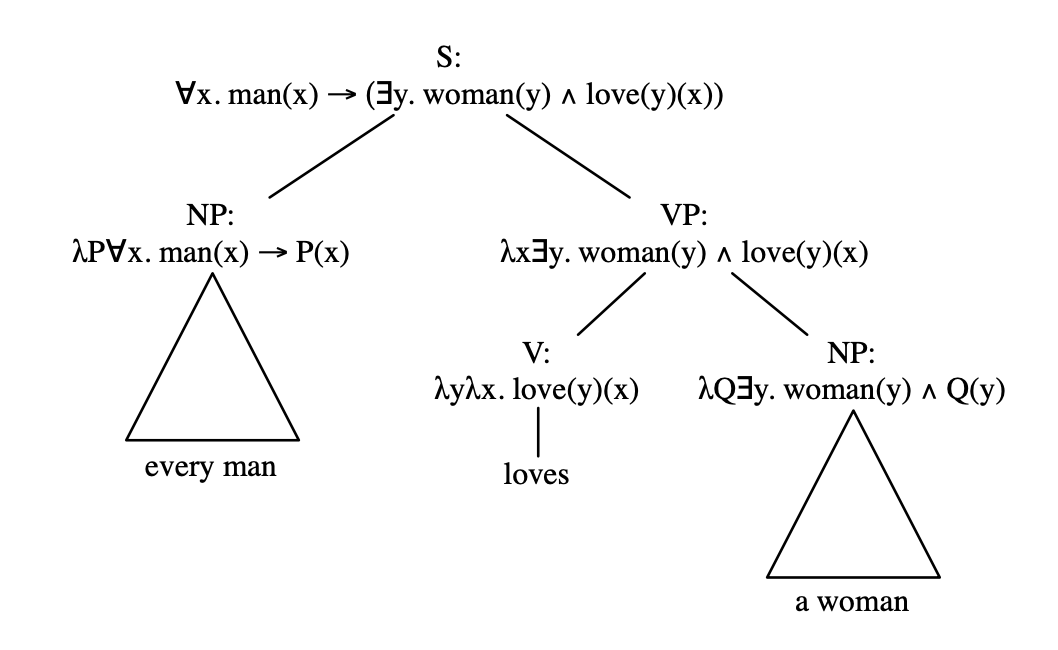
\includegraphics[width=10cm]{images/lambda_form.png}
	\caption[Lambda form]{A Montague-style \parencite{montague_1973} derivation of a semantic representation for the sentence “Every man loves a woman.” Credits: by Alexander Koller and Manfred Pinkal \url{https://www.coli.uni-saarland.de/~koller/papers/sem-handbook.pdf}}
	\labfig{lambda-form}
\end{figure}

There is this strong \bcomment{intuition}{hypothesis} \bcomment{in natural language processing}{computational linguistics} that language has a recursive structure \parencite{chomsky_56, shen_19}. As illustrated in \reffig{lambda-form} computing sentence semantic representations traditionally calls for a recursive compositional function whose structure is tree-shaped. Using syntax driven semantic analysis \parencite{jurafsky_2009}, we can map a sentence to a logical form that reflects its meaning—following the definition from \refsec{meaning:formal}. In this perspective, \bcomment{nonsense}{} we compute the sentence meaning using the compositionality principle. In its essence, the principle states that we can draw the meaning of a sentence by composing the meaning of its parts. \bcomment{That's an operational statement}{} We first infer the sentence structure\sidenote{The structure may consist in various trees such as constituency, dependency or binary parses.}. We then recursively compute the semantic representation along the structure, by \bcomment{rephrase the sentence}{} augmenting and combining each node with semantic attachments. These attachments follow explicit combination rules.

\begin{figure}[htb!]
	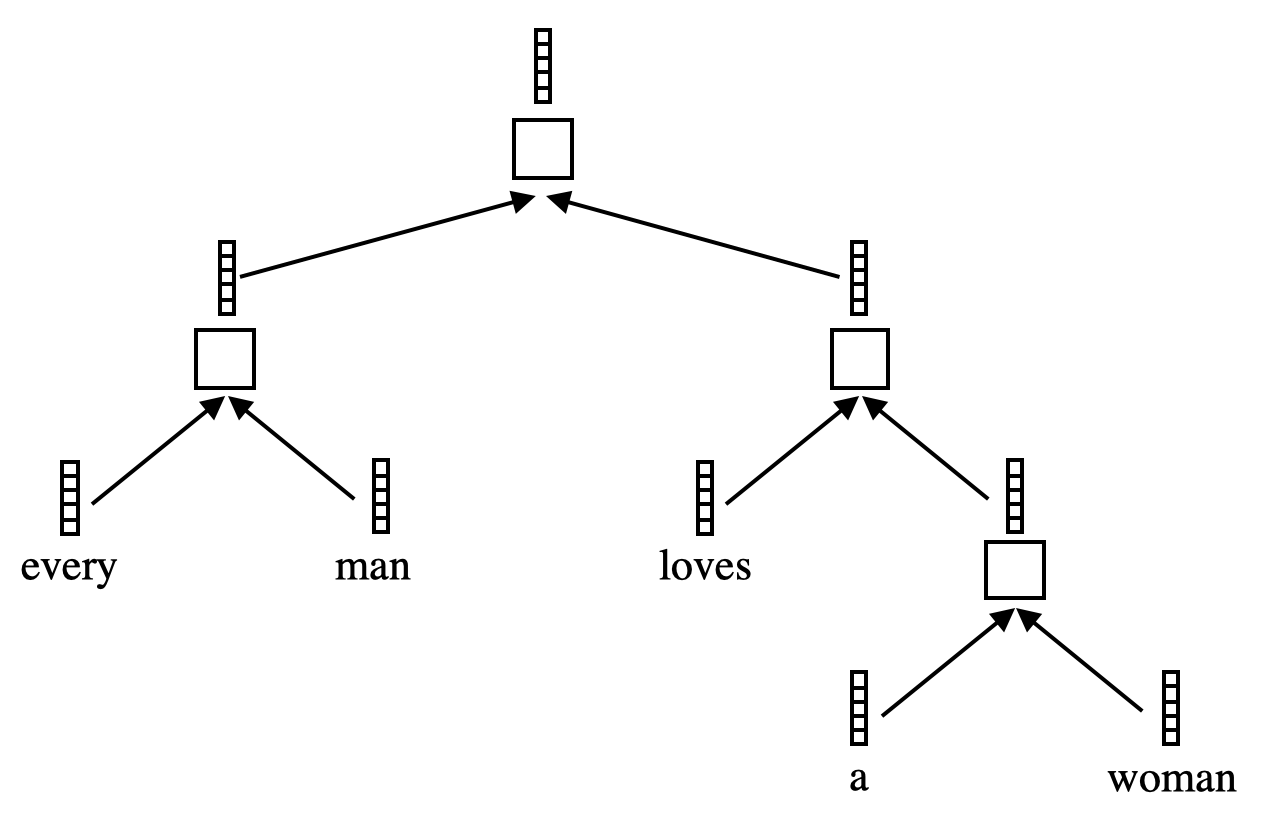
\includegraphics[width=10cm]{images/tree_rnn.png}
	\caption[Tree LSTM]{Semantic encoding of a sentence using a tree-structured neural model.}
	\labfig{tree-rnn}
\end{figure}

% As detailed in \refsec{training:architectures}, computing sentence semantic representations traditionally calls for a recursive compositional function whose structure is tree-shaped. 
\bcomment{}{\sidenote{Yep. the neural models cannot handle quantification naturally. Change the example to sentiment analysis and maybe refer to previous chapters on differences between logical representations and neural representations. Problematize : You might also state what gains you expect from structuring a neural model with a tree shape rather than using say an LSTM.}} Neural models can emulate this composition procedure using tree-structured networks. As for the logical form, such models proceed in two stages: first we infer the syntactic structure of the sentence, then we recursively compose the semantic representation along the structure. We illustrate the composition procedure in \reffig{tree-rnn}. Here, the semantic representations consist of vectors composed with linear algebra operations—as detailed in \refsec{meaning:distributional}. The parameters of the semantic algebraic operators are \textit{learned} by optimizing a loss function given a dataset. Regarding the sentence structure, we usually infer it using a dedicated parser, learned on labeled data.

% and enable better generalization and abstraction properties.

%%%%%%%%%%%%%%%%%%%%%%%%%%%%%%%%%%%%%%%%%%%%%%%%%%%%%%%%%%%%%%%%%%%%%%%%%%%%%%%%
\section{Latent tree learning}
%%%%%%%%%%%%%%%%%%%%%%%%%%%%%%%%%%%%%%%%%%%%%%%%%%%%%%%%%%%%%%%%%%%%%%%%%%%%%%%%

\bcomment{not really true}{in the supervised setting} Tree-based models need carefully hand-annotated data to be trained. One method of overcoming this limitation is to induce trees from raw text and computes semantic representations along with the inferred structure. Such methods preserve explicit recursive computation and produce intelligible tree structures. The learning method is called \textit{latent tree learning}, and it \bcomment{usually}{that's not usual} consists of two components: a parser and a \textsc{TreeLSTM} that uses those parses. The parser and composition function are learned jointly and are specific to a given task or domain. 

% All models differ from the syntactic formalism used and the training method.

The first set of latent tree models introduces an intermediate objective to train the parser component. \textcite{socher_11c} parse the sentence by selecting and merging adjacent nodes. The parser model is trained using an auxiliary reconstruction task. The Shift reduce Parser-Interpreter Neural Network (SPINN) model from \textcite{bowman_16} obtains the structure using a shift-reduce parser. The parser component also uses an intermediate objective that compares parses with gold-standard trees.

\textcite{maillard_19} introduce a model entirely trainable using backpropagation. However, the model does not rely on a soft structure and does not maintain the discreteness of the tree composition process\bcomment{a bit elliptic. what do they do really ?}{more details would be welcome}. It is, therefore, memory intensive as it explicitly computes a whole forest of 
% $\smallO{N^2}$ 
potential trees. 
%for $N$ words

\textcite{yogatama_17} adapt \textsc{SPINN} and jointly train its parsing and sentence embedding components. The model produces a discrete structure, but the resulting architecture is not fully differentiable and must thus be trained using a reinforcement learning proxy objective, limiting the convergence speed. \textcite{choi_18} compute a single tree instead of combinations from partial trees by using the Gumbel-Softmax estimator. The input is greedily and sequentially parsed.

\bcomment{overall at the end of this section, I miss some more details on what these guys really do. It requires to read the papers to get an idea. Lacks of self containment}{}


% a reconstruction error in \citet{socher_11c} and a comparison with gold-standard trees in \citet{bowman_16}.}

%A \treelstm{} is then applied on the parse to embed the sentence. But both models train the parser with an auxiliary task.
%: a reconstruction error and a comparison with gold-standard trees.

% \citet{bowman_16} introduce the Shift-reduce Parser-Interpreter Neural Network (SPINN). However as in \cite{socher_11c} the model train the parsing module with an auxiliary loss to match gold-standard trees. 

%%%%%%%%%%%%%%%%%%%%%%%%%%%%%%%%%%%%%%%%%%%%%%%%%%%%%%%%%%%%%%%%%%%%%%%%%%%%%%%%%%%%%%%%
% 2. Yogatama
%%%%%%%%%%%%%%%%%%%%%%%%%%%%%%%%%%%%%%%%%%%%%%%%%%%%%%%%%%%%%%%%%%%%%%%%%%%%%%%%%%%%%%%%

% \citet{yogatama_17} is the first model to jointly train its parsing and sentence embedding components. They base their model on shiftreduce parsing. Their parser is not differentiable, so they rely on reinforcement learning for training.

% \citet{yogatama_17} adapt the Spinn modelwith the REINFORCE algorithm. \citet{yogatama_17} introduce reinforcement learning to achieve the desired effect of discretization. However, slow convergence due to the reinforcement learning setting is one of its draw- backs, according to the authors.

%%%%%%%%%%%%%%%%%%%%%%%%%%%%%%%%%%%%%%%%%%%%%%%%%%%%%%%%%%%%%%%%%%%%%%%%%%%%%%%%%%%%%%%%
% 4. Maillard
%%%%%%%%%%%%%%%%%%%%%%%%%%%%%%%%%%%%%%%%%%%%%%%%%%%%%%%%%%%%%%%%%%%%%%%%%%%%%%%%%%%%%%%%
% \citet{maillard_19} propose an alternative approach, inspired by CKY parsing. The algorithm is made differentiable by using a soft-gating approach, which approximates discrete candidate selection by a probabilistic mixture of the constituents available in a given cell of the chart. This makes it possible to train with backpropagation.

% \citet{maillard_19} present a model, entirely trainable using  backpropagation — which explicitly computes O(N2) possible tree nodes for N words, and uses a soft gating strategy to approximately select valid combinations of these nodes that form a tree. Though their model reduces the ambiguity by explicitly representing a node as a weighted sum of all candidate compositions, it is memory intensive since the number of candidates linearly increases by depth.
% \textcolor{blue}{}

%%%%%%%%%%%%%%%%%%%%%%%%%%%%%%%%%%%%%%%%%%%%%%%%%%%%%%%%%%%%%%%%%%%%%%%%%%%%%%%%%%%%%%%%
% 5. Choi
%%%%%%%%%%%%%%%%%%%%%%%%%%%%%%%%%%%%%%%%%%%%%%%%%%%%%%%%%%%%%%%%%%%%%%%%%%%%%%%%%%%%%%%%

% \citet{choi_18} use an approach similar to easy-first parsing. The parsing decisions are discrete, but the authors use the Straight-Through Gumbel-Softmax estimator to obtain an approximate gradient and are thus able to train with backpropagation.

% \citet{choi_18} present a model (ST-Gumbel) that uses a similar data structure and gating strategy to \citet{maillard_19}, but which uses the Straight-Through Gumbel-Softmax estimator. This allows them to use a hard categorical gating function, so that their output sentence vector is computed according to a single tree, rather than a gated combination of partial trees as in \citet{maillard_19}.

% \textcolor{blue}{ \citet{choi_18} compute a single tree instead of combinations from partial trees by using the Straight-Through Gumbel-Softmax estimator. The input is greedily and sequentially parsed.}
% . However, \citet{choi_18} model iterates through $N - 1$ steps to build a tree over $N$ words, }

%%%%%%%%%%%%%%%%%%%%%%%%%%%%%%%%%%%%%%%%%%%%%%%%%%%%%%%%%%%%%%%%%%%%%%%%%%%%%%%%%%%%%%%%
%. 6. Williams
%%%%%%%%%%%%%%%%%%%%%%%%%%%%%%%%%%%%%%%%%%%%%%%%%%%%%%%%%%%%%%%%%%%%%%%%%%%%%%%%%%%%%%%%
% \citet{williams_18} investigate the trees produced by \citet{yogatama_17} and \citet{choi_18} when trained on two natural language inference corpora. They find that the former model induces almost entirely leftbranching trees, while the latter performs well but has inconsistent trees across re-runs with different parameter initializations.

% However, \citet{williams_18} empirically show that, Gumbel softmax produces unstable latent trees with the same hyper-parameters but different initializations, while reinforcement learning even tends to generate left-branching trees. Neither gives meaningful latent trees in syntax, but each method still obtains considerable improvements in performance. This indicates that syntax may not be the main contributor to the performance gains.
% We obtain a score close to the {\sc Spinn} model but without an explicit parsing objective. Rather we pre-trained the parsing model on the Penn Tree Bank and fine-tuned it on the SNLI task.

\textcite{williams_18} investigate the latent trees produced by \textcite{yogatama_17} and \textcite{choi_18} and show neither method produces meaningful syntactic representations. Gumbel softmax outputs inconsistent trees across initializations while reinforcement learning outputs trivial left-branching trees.


% We organized our paper as follows: after presenting the related in work in Section~\ref{sec:related-work}, we present our model in Section~\ref{sec:model}. 
% We then study the relevance of this framework for semantic inference and analyze the properties of such tree-structured models for downstream tasks. 
% In Section~\ref{sec:eval}, we evaluate our model on textual entailment and semantic similarity tasks. Regarding the textual similarity task, we show that our setup is competitive with \bert base, although the latest is trained on datasets many orders of magnitude larger. We then conduct an ablation study and analyze the impact of the parser initialization. In Section~\ref{sec:parses-impact}, we compare the learned structures across initializations and with interpretable annotations. In Section~\ref{sec:dowstream-impact} we study how latent structures impact performances on downstream tasks.
% with a significantly smaller training set.

% I focus on tree-structured neural networks, which naturally encode the structure of language. For each sentence, the network computes text units following a syntactic tree, starting from the leaf nodes, up to the root. However, such models suffer from practical constraints that limit their application. In particular, tree-based models not only require raw text as input but also the sentence structure in the form of a parse tree. Such structure may be tedious to obtain as it requires manual annotations and external parsers. To overcome such limitations, I formulated a novel tree-based model that learns its composition function together with its structure \parencite{simoulin_2020}. The model includes two modules, a biaffine graph parser, and a Tree-LSTM. The parsing and the composition functions are explicitly connected and, therefore, learned jointly. The method differs from previous work as the representation is not computed from the whole forest of potential trees. Moreover, training the full model directly does not require supervision from a parsing objective. The model outperforms tree-based models relying on external parsers on downstream tasks. In some configurations, it is even competitive with BERT-base model.

\section{Unified parsing and compositional model}
\labsec{sec:model}

% However, architectures often have practical limitations, requiring either complex learning paradigm such as reinforcement learning \parencite{yogatama_17} or intensive computations \parencite{maillard_19}.
Architectures listed above  have practical limitations, requiring either complex learning paradigm such as reinforcement learning, intensive computations or requiring an external parser module.

% To limit the need for an external parser, w
We propose a unified architecture, which infers an explicit tree structure and trains recursively a sentence embedding model. Our method is fully differentiable and relies on existing and well-known components. We use a standard dependency parsing structure, obtained using a graph-based biaffine dependency parser \parencite{dozat_17}. However, our model is not limited to a particular parser architecture as long as it is differentiable. This flexibility gives us the freedom to explore the impact of the parser choice. \bcomment{apparent contradiction, you said earlier that using an external parser is a weakness}{}

\bcomment{}{State more clearly that you designed a joint model by contrasting with others} Our model performs jointly sentence parsing and the prediction of a sentence embedding. The sentence embedding is predicted by a \bcomment{weighted}{why weighted ?} \textsc{TreeLSTM} whose tree structure is provided by a dependency parser.
The \textsc{TreeLSTM} recursive composition function crucially uses a weighted sum of the child representations whose weights are provided by the parser edges, hence linking the parser outputs to the \textsc{TreeLSTM} recursion.
% \footnote{The model is illustrated in Appendix~\ref{sec:figure}.}.

\paragraph{Parsing model} The parser is a standard graph based biaffine dependency parser \parencite{dozat_17}.
It is formalized in two steps.
First, in Eq. \ref{eq:biaffine-1} to \ref{eq:biaffine-3},
it computes a weight matrix that is interpreted as weighted directed graph whose nodes are the sentence tokens:
%\par\noindent{\small
\begin{align}
   \text{Biaff}(x_1,x_2) &=  x_1^T U x_2 + W^{(b)}(x_1 \oplus x_2)+b^{(b)} \\
    a_k^{(dep)} &= W^{(dep)}h_k + b^{(dep)} \label{eq:biaffine-1} \\
    a_j^{(head)} &= W^{(head)}h_j + b^{(head)} \label{eq:biaffine-2}\\
    s^{(arc)}_{kj} &= \text{Biaff}(a_k,a_j) \label{eq:biaffine-3}
\end{align}%}
The second step performs parsing by computing a maximum spanning tree from the graph. As in \textcite{dozat_17}, we use the Max Spanning Tree (MST) algorithm \bcomment{cite Edmonds as it is a non standard -directed- MST algorithm}{} to ensure the well-formedness of the tree: 
\begin{align}
 \alpha_{kj} &= \mathbb{1}_{mst(s^{(arc)}_{kj})} s^{(arc)}_{kj} \label{eq:biaffine-alpha}
\end{align}
Where $\alpha_{kj}$ is the probability of the edge linking node $j$ to node $k$. For a given node $k$, there is at most one non-zero edge leading to its governor $j$.
% weighted edge

\paragraph{Compositionally weighted tree LSTM} Given a predicted tree structure, we recursively encode the sentence using a variant of the Child Sum Tree model from \textcite{tai_15} detailed below:
% \par\noindent{\small
\begin{align}
\tilde{h}_j &= \sum_{k \in C(j)} \alpha_{kj} h_k, \label{eq:treelstm-weighted} \\
%\tilde{h}_j &= \sum_{k \in C(j)} h_k, \label{eq:treelstm-first} \\
i_j, o_j, u_j &=\sigma \Big( W^{(i, o, u)} x_j + U^{(i, o, u)} \tilde{h}_j + b^{(i, o, u)} \Big), \\
% o_j &= \sigma \left( W^{(o)} x_j + U^{(o)} \tilde{h}_j  + b^{(o)} \right), \\
% u_j &= \tanh\left( W^{(u)} x_j + U^{(u)} \tilde{h}_j  + b^{(u)} \right), \\
f_{jk} &= \sigma\left( W^{(f)} x_j + U^{(f)} h_k + b^{(f)} \right), \label{eq:treelstm-f}\\
c_j &= i_j \odot u_j + \sum_{k\in C(j)} f_{jk} \odot c_{k}, \\
h_j &= o_j \odot \tanh(c_j), \label{eq:treelstm-last}
\end{align}
%}
Where in Eq.~\ref{eq:treelstm-weighted}, $C(j)$ denote the set of children of node $j$.
% and $k \in C(j)$. 
Crucially, in our case, Eq.~\ref{eq:treelstm-weighted} is a weighted sum rather than a standard sum and the weights are those $\alpha_{kj}$ provided by the parser.

%\paragraph{Discussion}
We use the embedding computed by the weighted \textsc{TreeLSTM} at the root of the tree as the sentence embedding.
% The core model outputs a sentence embedding computed by a weighted \treelstm{}.  
% a compositionnaly weighted tree-{\sc lstm}
The tree shape and the edge weights are given by the best prediction of a graph parser. The parsing model is linked to the \textsc{TreeLSTM} by the weights $\alpha_{kj}$. This architecture allows us to update jointly the parser and the \textsc{TreeLSTM} weights using only the downstream task loss. The supervision comes only from the objective of the downstream task, and no intermediate structure target is required.
%our model supervision only appears in the semantic objective and no intermediate structure target is required. 
% the architecture allows us to update the parser and \treelstm{} weights using solely the loss provided by the downstream task. 

% It therefore differs from models like {\sc Spinn} \cite{bowman_16}, which includes direct supervision from a parsing objective.

% The method described here differs from previous work as the representation is not computed from the whole forest of potential trees \citep{yogatama_17, maillard_19, williams_18, shen_18, liu_18} but instead on the single best tree while being completely differential. Thus, it can be trained using back-propagation on a supervised task for which we want to provide relevant sentence embeddings. The architecture is, in principle, generic and adaptable to any other downstream task. 

Our model, illustrated in \reffig{biaffine-tree-lstm}, is fully differentiable and preserve the discreteness of the tree composition process. It relies on a dependency parsing formalism and could accommodate any \bcomment{differentiable}{Let's talk about differentiabiliy\ldots} parser.

\begin{figure}[!ht]
	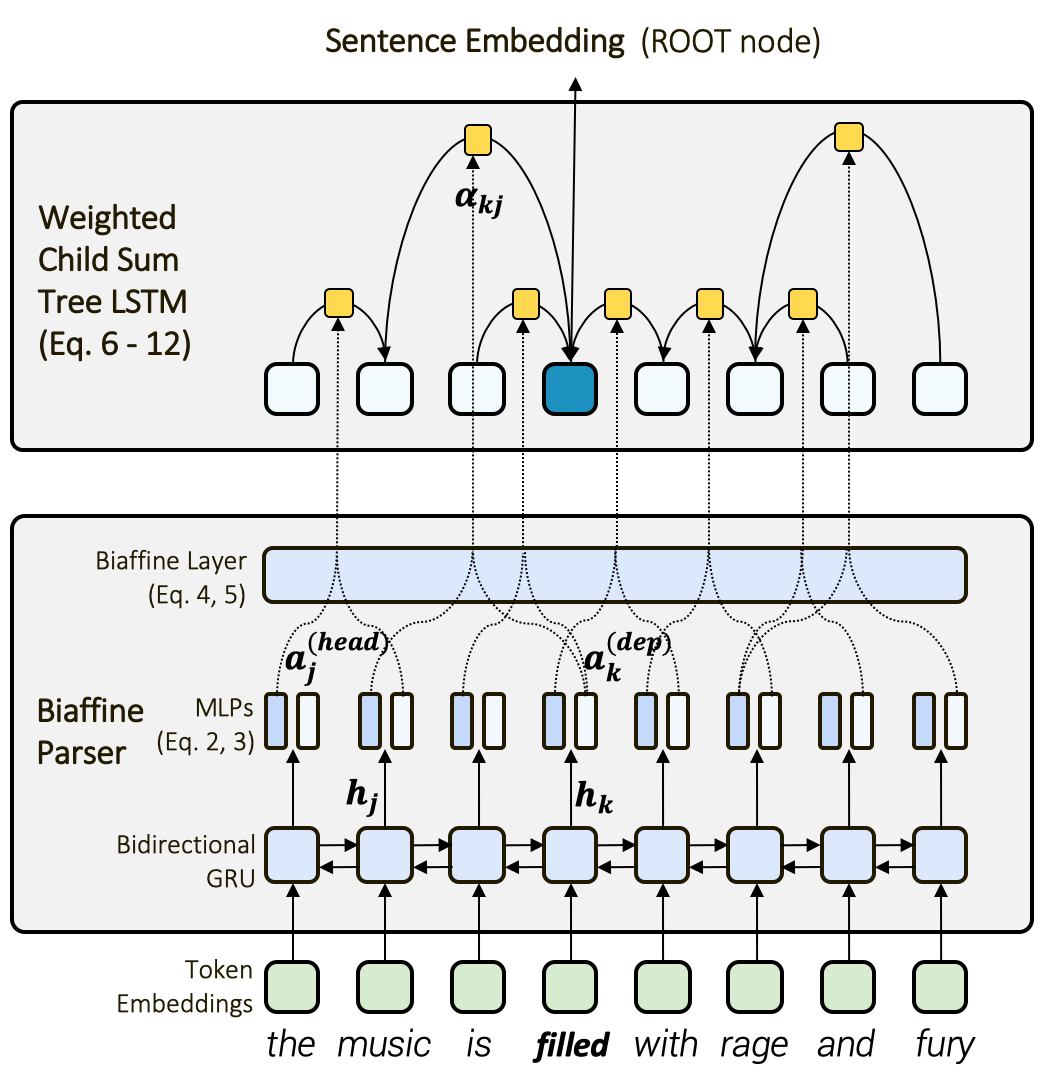
\includegraphics[width=7cm]{images/biaffine-12.png}
	\caption[Biaffine tree lstm]{We illustrate the architecture detailed in Eq. \ref{eq:biaffine-1} to \ref{eq:treelstm-last}. The Biaffine parser provides the sentence structure from which the \textsc{TreeLSTM} computes sentence embeddings. The full pipeline is differentiable as the \textsc{TreeLSTM} weights are given by the parser.}
	\labfig{biaffine-tree-lstm}
\end{figure}

%%%%%%%%%%%%%%%%%%%%%%%%%%%%%%%%%%%%%%%%%%%%%%%%%%%%%%%%%%%%%%%%%%%%%%%%%%%%%%%%
\section{Evaluation on downstream tasks}
\labsec{sec:eval}
%%%%%%%%%%%%%%%%%%%%%%%%%%%%%%%%%%%%%%%%%%%%%%%%%%%%%%%%%%%%%%%%%%%%%%%%%%%%%%%%

Our architecture primarily aims to produce relevant embeddings for downstream tasks. To this end, we compare our setup with other models from the literature on various tasks. For this comparison, we first pre-train the parsing submodel on human-annotated sentences from the Penn Tree Bank (PTB) \parencite{marcus_94} converted to Stanford dependencies. We then fine-tune the parser's parameters on the task while training the full model\sidenote{In this configuration, we observe pre-training the parser may cause weights $\alpha$ to become too large in Eq. \ref{eq:biaffine-alpha}. This leads to poor downstream performances. We correct this with a multiplicative parameter $\tau$ whose value is estimated during training. It means we replace Eq. \ref{eq:biaffine-alpha} with: $\alpha_{kj} = \tau \cdot \mathbb{1}_{mst(s^{(arc)}_{kj})} s^{(arc)}_{kj}$ for tree weights computation.}.


\subsection{Semantic textual similarity (STS)}
\label{sec:sts}

We first evaluate our model on the SICK-R downstream task \parencite{marelli_14}, which is dedicated to assessing models' compositional properties. 
%The task intends to discriminate models that rely on shallow lexical pattern matching from those that take advantage of the sentence underlying structure. 
The dataset comprises 9,927 sentence pairs, distributed in a 4,500/500/4,927 train/dev/test split, annotated for semantic similarity on a 1 to 5 real range. It includes specific examples of variations on passive and active forms, quantifier and modifier switches, or negations. 
%This is a SentEval task \cite{conneau_18} specifically
\bcomment{to get a more self contained doc you might present the task with slightly more details, provide examples etc.}{}


\paragraph{Training configuration}

\bcomment{with more details on the task, the following parag would be easier to understand}{}
We use a similar training procedure
%\footnote{Hyperparameters such as hidden size, optimization procedure such or learning rate are fixed as proposed in \citet{tai_15} and are detailed in Appendix.} 
as in \textcite{tai_15}. We transform the target $y$ from the SICK-R task into the distribution $p$ defined by:

\begin{equation*}
p_{i} = \left\{
\begin{array}{ll}
y - \lfloor{y}\rfloor, & i = \lfloor{y}\rfloor + 1 \\
\lfloor{y}\rfloor - y + 1, & i = \lfloor{y}\rfloor \\
0 & \text{otherwise}
\end{array} \right.
\end{equation*}
We use a dedicated architecture to predict the similarity distribution from a pair of sentences. The similarity module takes as input a pair of sentence vectors $h_{L} $ and $h_{L}$ and computes their component\-wise product $h_{L} \odot h_{R}$ and their absolute difference $|h_{L} - h_{R}|$. Given these features, we compute the probability distribution  $\hat{p}_{\theta}$ using a two layers perceptron network (MLP):
\begin{align}
\begin{split}
&h_{\times}=h_L\odot h_R, ~~~~~h_{+} = |h_L - h_R |, \\
&h_s = \sigma (W^{(\times)}h_{\times} + W^{(+)}h_{+} + b^{(h)}), \\
&\hat{p}_{\theta} = \text{softmax}(W^{(p)}h_s + b^{(p)}),\\
\end{split}
\end{align}
Where $\sigma$ is the sigmoid function. We use the KL-divergence between the prediction $\hat{p}_{\theta}$ and the ground truth $p$ as training objective:
\begin{equation}
J(\theta) = \frac{1}{N}\sum_{k=1}^{N}\text{KL}(p^{(k)} || \hat{p}_{\theta}^{(k)}) + \lambda||\theta||_{2}^{2}
\end{equation}
Finally during inference, the similarity score $\hat{y}$ is computed as $\hat{y} = r^{\intercal} \hat{p}_{\theta}$ with $r^{\intercal} = [1, \dots, 5]$. 

% We use a standard training configuration, inspired from \citet{tai_15} and combine the embeddings obtained with our model for each sentence with a similarity module\footnote{The setup is detailed in Appendix \ref{sec:sick-train}.}.

\paragraph{hyper-parameters} \bcomment{We set the hyperparameters given literature on the domain}{reformulate}, in particular regarding choices made in \textcite{tai_15}. For all experiments detailed in the current Section, the batch size is fixed to 25, weight decay to $1e^{-4}$ and gradient clipping set to $5.0$. The learning rate is set to $0.025$ for the \textsc{TreeLSTM} parameters. When using a pre-training procedure for the parser, we set the learning rate to $5e^{-3}$ and use the following warm-up: for the first epoch, the parser is frozen. For the following epochs, all parameters are trained. At each epoch, the parser learning rate is divided by a factor of two. Without pre-training, the learning rate is set to $5e^{-4}$ for the parser. All model weights are initialized with a Xavier distribution. The hidden size of the similarity architecture is set to 50. The \textsc{TreeLSTM} hidden size is set to 150. We use the Adagrad optimizer. We do not apply any dropout. We perform training for a maximum of 20 epochs and stop when no improvement was observed on the development set for 3 consecutive epochs.
%  and biases set to 0
Regarding the vocabulary, we limit the size to 20,000 words and initialize the embeddings layer with 300-dimensional GloVe embeddings\sidenote{\url{https://nlp.stanford.edu/projects/glove/}}. The embeddings are not updated during training\sidenote{We trained all models on a single 1080 Ti Nvidia GPU. Training time for each epoch is approximately 1 minute. The model counts 13.7M parameters. Data can be downloaded using the SentEval package \url{https://github.com/facebookresearch/SentEval}.}.

% We set the hyper-paremeter given literature on the domain, in particular regarding choices made in \citet{tai_15}. We detail the full setup in Appendix  \ref{sec:sick-train}.

% \subsection{Comparison with other encoders} 
% \label{sec:soa}

Table \ref{table:supervised} reports the results from the test set. As expected, structured models perform better than models using weaker underlying structures. We also observe that our model is competitive with a \textsc{Bert}-base upper-line. It is essential to note that \textsc{Bert} models are heavily pre-trained on vast corpora, whereas our structured models are trained only on the SICK-R and PTB data. 

% Moreover, our model achieves a significantly lower standard variation than {\sc bert}-base implementation.
\begin{table}[!htb]
\centering
\small
\begin{tabularx}{\textwidth}{@{}Y | c@{} }
\toprule
\textbf{Encoder} & \textbf{$r$} \\
\midrule
\midrule 
\textsc{Bow}$^\dagger$ & 78,2 \scriptsize{(1,1)} \\
% \midrule 
\textsc{LSTM}$^\dagger$ & 84.6 \scriptsize{(0.4)}  \\
Bidirectional \textsc{LSTM}$^\dagger$ & 85.1 \scriptsize{(0.4)} \\
% \midrule
N-ary \textsc{TreeLSTM}$^\dagger$ \parencite{tai_15} & 85.3 \scriptsize{(0.7)} \\
Childsum \textsc{TreeLSTM}$^\dagger$ \parencite{tai_15} & 86.5 \scriptsize{(0.4)}  \\
% \midrule
\textsc{Bert}-base \parencite{devlin_19} & 87.3 \scriptsize{(0.9)} \\
% \bert{}-large & 89.4 \scriptsize{(0.6)} & 84.7 \scriptsize{(1.0)} & 21.5 \scriptsize{(1.3)} \\
\midrule
\multicolumn{2}{c}{\textit{Our model}}\\
\midrule
% Unified \treelstm{}$^\dagger$ (\textbf{our model)} & 87.0 \scriptsize{(0.3)} \\
Unified \textsc{TreeLSTM}$^\dagger$ & 87.0 \scriptsize{(0.3)} \\
% Unified \treelstm{}-100 & 86.5 \scriptsize{(0.2)} & 80.4 \scriptsize{(0.4)} & 25.9 \scriptsize{(0.5)} \\
\bottomrule
\end{tabularx}
\caption{Evaluation of the model on the SICK-R task: we pre-train our parsing module on the PTB and continue to update the full model on the SICK-R task. We compare with \textsc{Bert} and models relying on sequential and tree structures. We report Pearson correlation on the test set, by convention as $r \times 100$ (average and standard deviation from 5 runs). $\dagger$ indicates models that we trained.}
% \textbf{(1)} No underlying structure 
\label{table:supervised}
\end{table}

\subsection{Textual entailment}
\label{sec:ste}

We also test our model on the Stanford Natural Language Inference (SNLI) task \parencite{bowman_15}, which includes 570k pairs of sentences with the labels entailment, contradiction, and neutral. It is distributed in a 550k/10k/10k train/dev/test split. 
\bcomment{self containment}{provide some more details. what are the inputs, the outputs ?}

\paragraph{Training configuration}

We use a similar training procedure as in \textcite{choi_18}. A dedicated architecture is used to predict the similarity distribution from a pair of sentences. The similarity module takes as input a pair of sentence vectors $h_{L} $ and $h_{L}$ and computes their component\-wise product $h_{L} \odot h_{R}$ and their absolute difference $|h_{L} - h_{R}|$. Given these features, we compute the probability distribution  $\hat{p}_{\theta}$ using a three layers perceptron network (MLP):
\begin{align}
\begin{split}
&h_{\times}=h_L\odot h_R, ~~~~~h_{+} = |h_L - h_R |, \\
&h_s = \textsc{Relu}(W^{(1)}[h_{\times}, h_{+}, h_L, h_R] + b^{(1)}), \\
&h_s = \textsc{Relu}(W^{(2)}h_s + b^{(2)}), \\
&\hat{p}_{\theta} = \text{softmax}(W^{(p)}h_s + b^{(p)}),\\
\end{split}
\end{align}
We use the cross entropy loss between the prediction $\hat{p}_{\theta}$ and the ground truth $p$ as training objective:
\begin{equation}
J(\theta) = -\frac{1}{N}\sum_{k=1}^{N}p^{(k)} log \hat{p}_{\theta}^{(k)} + \lambda||\theta||_{2}^{2}
\end{equation}

% We use a standard training configuration, inspired from \citet{choi_18} for which a similarity module is used to combine the embeddings obtained with our model for each sentence\footnote{The setup is detailed in Appendix \ref{sec:snli-train}.}. 

% We choose a standard training configuration, inspired from \citet{bowman_15} for which a similarity modules is used to combine the embeddings obtained with our model for each sentence\footnote{The setup is detailed in Appendix \ref{sec:sick-train}.}.  We report the corresponding results from the test set in Table \ref{table:supervised}.

%We set the hyper-paremeter given literature on the domain, in particular regarding choices made in \citet{choi_18}. We detail the full setup in Appendix  \ref{sec:snli-train}.

\paragraph{hyper-parameters} \bcomment{We set the hyper-parameters given literature on the domain}{reformulate}, in particular regarding choices made in \textcite{choi_18}. For all experiments detailed in Section \ref{sec:ste}, the batch size is fixed to 128, weight decay to $0$, and gradient clipping set to $5.0$. The learning rate is set to $1e^{-3}$ for the \textsc{TreeLSTM} and the parser. The hidden size of the similarity architecture is set to 1024. The \textsc{TreeLSTM} hidden size is set to 600. We use the Adam optimizer. We apply a 0.2 dropout within the similarity architecture. We perform training for a maximum of 20 epochs and stop when no improvement was observed on the development set for 3 consecutive epochs.
Regarding the vocabulary, we limit the size to 100,000 words \bcomment{why a different setup than earlier ?}{} and initialize the embeddings layer with 300-dimensional GloVe embeddings. The embeddings are not updated during training. % \cite{pennington_14}

\begin{table}[!htb]
  \centering
  \small
  \begin{tabularx}{\textwidth}{@{}Y | c@{} }
    \toprule
    \textbf{Encoder} & \textbf{Test Acc.} \\
    \midrule
    \midrule 
    % {\sc LSTM} \cite{bowman_16} & 77.6 \\
    % \midrule
    \textsc{Spinn} \textbackslash w Reinforce \parencite{yogatama_17} & 80.5  \\
    CYK and \textsc{TreeLSTM} \cite{maillard_19} & 81.6  \\
    \textsc{Spinn} \parencite{bowman_16} & 83.2 \\
    % \midrule
    % Syntactic TreeLSTM \cite{chen_17} & 93.5 & 88.6 \\
    % MT-DNN \cite{liu_19} & 97.2 & 91.6 \\
    ST-Gumbel \parencite{choi_18}  & 86.0 \\
    Structured Alignment \parencite{liu_18} & 86.3 \\
    \textsc{Bert}-base \parencite{zhang_20} & 90.7 \\
    % {\sc SemBert}-base \cite{zhang_20} & 91.0 \\
    \midrule
    \multicolumn{2}{c}{\textit{Our model}}\\
    \midrule
    % Unified \treelstm{} (\textbf{our model}) & 85.0 {\scriptsize (0.2)} \\
    Unified \textsc{TreeLSTM} & 85.0 {\scriptsize (0.2)} \\
    % Unified \treelstm{} \textbackslash w tracking \textsc{LSTM} (\textbf{ours}) & 83.0 {\scriptsize (0.8)} \\
    % Unified \treelstm{}-100 & 83.6 {\scriptsize (0.0)} \\
    \bottomrule
  \end{tabularx}
  \caption{Evaluation of the model on the SNLI-R task: We pre-train our parsing module on the PTB and continue to update the full model on the SNLI task. We compare with \textsc{Bert} and latent tree learning models. We report the accuracy on the test set (average and standard deviation from 2 runs).}
  % Comparison with other models on the \textbf{SNLI} task. Results are grouped as follow: \textbf{(1)} Sequential structure \textbf{(2)} Model learning tree structures \textbf{(3)} Framework introducing a direct interaction between the premise and hypothesis using attention mechanism \textbf{(4)} Our model with a pre-training on the PTB. We report the average and the standard deviation from 2 runs.}
  \label{table:snli}
\end{table}

We report the results in Table \ref{table:snli}. Our results are close to \textcite{choi_18}, which also compute semantic representations along to discrete tree structures but relies on a distinct syntactic formalism. \bcomment{conjecture what explains the differences ?}{}

In models from \textcite{liu_18} and \textcite{zhang_20} sentences are encoded with direct interaction using an attention mechanism. These architectures relying on cross sentence attention outperform those without.
% , but our work focuses on the underlying sentence structure
We hypothesize that, 
% for the semantic similarity task, the final prediction could be extrapolated from both sentence embeddings. In such a case, the model was competitive with {\sc Bert}. 
on this textual entailment task, the final prediction cannot be directly deduced from both sentence embeddings. In this case, \textsc{Bert} and the structured alignment model have a clear advantage since they encode interactions between both sentences.
% Further work could involve adding such interactions as exemplified in \citet{liu_18}.}
% In the two first sections of Table~\ref{table:snli}, there is no intermediate interaction between the encoding of each sentence representation. In the second part of the Table, sentences are encoded with direct interaction using an attention mechanism. Models using interaction outperform those without, but our work focuses on the underlying sentence structure.
% \textcolor{blue}{To compare our results, we use a procedure analogue as in \citet{choi_18} and \citet{bowman_16} and apply a tracking \textsc{LSTM} on token input embeddings to give contextual information to each leaf node. 


% Our comparison includes models that induce direct interactions between sentences using attention mechanism. Such setup drastically improves the test accuracy.

% However, our focus lays on the sentence underlying structure rather than in the interaction between the premise and the hypothesis. In this perspective, we consider evaluation methods, as ours, do not introduce intermediate interaction between each sentence hidden representations. In this comparison, our model achieve an accuracy comparable to the {\sc Spinn} model. 


%  We aim at quantifying the degree of supervision needed to achieve competitive performance on downstream tasks with consistent syntactic structures.

% \subsection{Comparison with linguistic parse}
% \label{subsec:parse}

% \begin{itemize}

%%%%%%%%%%%%%%%%%%%%%%%%%%%%%%%%%%%%%%%%%%%%%%%%%%%%%%%%%%%%%%%%%%%%%%%%%%%%%%%%%%%%%%%%
\section{Impact of the parser initialization}
\labsec{sec:parser-init}
%%%%%%%%%%%%%%%%%%%%%%%%%%%%%%%%%%%%%%%%%%%%%%%%%%%%%%%%%%%%%%%%%%%%%%%%%%%%%%%%%%%%%%%%


Our framework primarily aims to be a structured sentence encoder. Accordingly, we have demonstrated in the previous Section that our architecture is competitive with comparable approaches and might even be competitive with \textsc{Bert}-based models. We are also interested in interpreting the structures the model actually learns and how such structures impact downstream performances.

In the previous experimental section, we pre-trained the parser on human annotated data. %Indeed, we expect the optimal structure to exhibit intuitive patterns such as subject-verb or verb-object connection. 
\bcomment{However, the optimal structure might differ from the task}{reformulate}. Moreover, for computational reasons, it might even differ significantly from linguistic insights. In this Section we perform an ablation study to better understand how the initialization of the parser impacts the resulting structures (Section \ref{sec:parses-impact}) and the final downstream performances (Section \ref{sec:dowstream-impact}). We begin by defining the different initialization scenarios we considered.

\paragraph{Linguistic annotations} Tree-structured models traditionally rely on linguistic structures obtained by parsers \parencite{tai_15}. For languages such as English, linguistic resources are available; it is technically possible to pre-train the parser. However, resources such as the PTB are not available in all languages. To better quantify the benefits of using linguistic annotations, we propose the following configurations, using various proportions of the PTB to initialize the parser:

\begin{itemize}
    \item In the \textbf{PTB-All} configuration, the parser is previously pre-trained on the PTB. This configuration is the same as in \refsec{sec:eval}.
    \item In the \textbf{PTB-$\emptyset$} configuration, the parser parameters are randomly initialized
    \item We also consider an initialization with only a small proportion of the \textbf{PTB} and train a parser by only using 100 randomly selected samples. This configuration is referred as \textbf{PTB-100}.
\end{itemize}


% Given the similarity of such attention matrices to the score matrices employed in arc-factored dependency parsing (Mc- Donald et al., 2005a,b), a salient question concern- ing interpretability becomes: Can we expect some combination of these parameters to capture linguis- tic structure in the form of a dependency tree, espe- cially if the model performs well on NLP tasks?

% With large-scale machine translation and language models being openly distributed for ex- perimentation, several researchers have wondered if self-attention is capable of representing syntactic structure, despite not being trained with any overt parsing objective.

%  Often, the line of in- quiry regarding interpretability in NLP has been concerned with extracting and analyzing linguistic information from neural network models of lan- guage (Belinkov and Glass, 2019). Recently, such investigations have targeted Transformer models (Hewitt and Manning, 2019; Rosa and Marecˇek, 2019; Tenney et al., 2019), at least in part because the self-attention mechanism employed by these models offers a possible window into their inner workings. With large-scale machine translation and language models being openly distributed for ex- perimentation, several researchers have wondered if self-attention is capable of representing syntactic structure, despite not being trained with any overt parsing objective.

% In pursuit of this question, Raganato et al. (2018) applied a maximum-spanning-tree algorithm over the attention weights of several trained MT models, comparing them with gold trees from Universal De- pendencies (Nivre et al., 2016, 2020). They found that, while the accuracy was not comparable to that of a supervised parser, it was nonetheless higher than several strong baselines, implying that some structure was consistently represented.

% These models often choose a Transformer architecture largely owing to its at- tractive scalability. Studies (Hewitt and Manning, 2019; Jawahar et al., 2019)  have shown that a pre- trained transformer is able to capture certain syn- tactic information implicitly by learning from suf- ficient examples. However, there is still a big gap between the syntactic structures implicitly learned and the golden syntax trees created by human ex- perts.

\paragraph{Unsupervised structures}\bcomment{transition à discuter}{} We are also interested in structures emerging from large pre-trained models. Such models present similarities with recent graph parser architecture. Although they are not trained with a direct parsing objective, many lines of work investigate if attention matrix can reflect syntactic structures \parencite{jawahar_19, clark_19, ravishankar_21} or, on the contrary, if it is efficient to integrate tree structural information within transformers \parencite{wang_19, bai_21}. 

As stated in the Introduction, our model is not specific to any parser architecture. It is, therefore, possible to use any model or heuristic to infer sentence structure. 
%We observed in the previous Section that parser initialized on only a sub-sample from the PTB lead to intelligible parses. In this Section we analyze to which extend it is possible to initialize the parser without linguistic insights.
In particular, we can use a pre-trained model such as \textsc{Bert} to infer structures based on the internal representation it learns.

%In this setup, we only use \bert{} to output a tree structure for the sentence. Word are then composed using our previously defined \treelstm{}. 
\textsc{Bert} relies upon the self-attention mechanism. Inside each layer, tokens are computed as a weighted combination from each other. For each token $x$, a query and key vector are computed using a linear transformation detailed in Eq~\ref{eq:qkv}. Given these vector tuples, the attention weights $s$ are computed following Eq~\ref{eq:bert-attention} in which $N$ refers to the dimension of the query and key vectors.

\begin{align}
    %h^0_j &= W_eu_j + W_p \label{eq:first-layer}\\
    q_j, k_j &= W^{(q, k)} x_j + b^{(q, k)} \label{eq:qkv}\\
    %s_{kj} &= \mathsf{softmax}\left(\frac{k_{k} \cdot q_{j}}{\sqrt{N}}\right) \cdot v_k \label{eq:bert-attention}
    s_{kj} &= \mathsf{softmax}\left(\frac{k_{k} \cdot q_{j}}{\sqrt{N}}\right) \label{eq:bert-attention}
    %h^n_j &= \sum_{k=1}^{N} \alpha_{kj} h^{n-1}_k \label{eq:bert-weighted}
\end{align}
% \quad \forall n \in [1, L]

We induce a tree structure following a procedure close from \textcite{ravishankar_21}. The method interprets the combination weights $s$ as a weighted graph whose nodes are tokens. We then apply Eq~\ref{eq:biaffine-3} to induce a maximum spanning tree from the attention matrix as detailed in \refsec{sec:model}. We make use of the last layer and induce a tree for each attention head taken separately. Given the tree structure induced from \textsc{Bert}, we apply our \textsc{TreeLSTM} model detailed in Eq. \ref{eq:treelstm-weighted} to \ref{eq:treelstm-last}. We stress the fact that in this configuration, we only use \textsc{Bert} as an unsupervised parser to infer a sentence structure. The semantic composition along with the structure to produce a sentence embedding is solely computed by the weighted \textsc{TreeLSTM}.\bcomment{you do not state how you combine the weights of the heads}{}

%\footnote{Parameters initialization is detailed in Appendix.}.
\bcomment{move this elsewhere}{}In both linguistic and unsupervised configurations, we either continue to update the parser when fine-tuning the model on downstream tasks or freeze the parser and only train the \textsc{TreeLSTM}. These two configurations are indicated with respectively \textbf{$\checkmark$} and \textbf{$\times$} symbols. 
% 


% \section{Experiments in low supervised setups}
\subsection{Impact of the initialization on parses}
\label{sec:parses-impact}


% However, we not interested solely in tackling downstream tasks, but also to produce consistent syntactic structures. Therefore, we focus in the next Section on the tree produced by our method.

\bcomment{structural issue}{introduce PTB 100 etc here}

In this Section, we analyze to which extend the structures generated by our model are comparable with meaningful linguistic annotations. We compare the parses generated by two distinct models differing by their initialization on the development set of both tasks. Our reference is the silver parses from the PTB-All configuration, where the parser is previously pre-trained on the full PTB and not updated during training.   

%We compare the learned parse with silver references to investigate the linguistic consistency of the learned structures. To this end, we contrast distinct configurations for which we initialize our parser with various degrees of supervision. 

In Table~\ref{table:parse}, we measure the Unlabeled Attachment Score (UAS) between the two parsers, that is, the ratio from the number of common arcs between two parses by the total number of arcs. 

\begin{table}[!htb]
\centering
\small
\begin{tabularx}{\textwidth}{@{}c c | Y Y@{}}
\toprule
\textbf{Parser 1} & \textbf{Parser 2} & \textbf{SICK-R (dev UAS)} & \textbf{SNLI (dev UAS)}\\
\midrule\midrule
\multicolumn{4}{c}{\textit{Impact of parser fine-tuning}}\\
\midrule
PTB-100 (\checkmark) & PTB-100 ($\times$) & 85.2 {\scriptsize (1.5)} & 5.6 {\scriptsize (1.9)}\\
PTB-All (\checkmark) & PTB-All ($\times$) & 98.4 {\scriptsize (0.1)} & 11.7 {\scriptsize (0.9)}\\
\midrule
\multicolumn{4}{c}{\textit{Impact of the PTB sample size}}\\
\midrule
PTB-100 (\checkmark) & PTB-$\emptyset$ (\checkmark) & 6.3 {\scriptsize (0.0)} & 10.1 {\scriptsize (10.7)}\\
PTB-All (\checkmark) & PTB-$\emptyset$ (\checkmark) & 10.1 {\scriptsize (0.0)} & 15.1 {\scriptsize (15.4)}\\
PTB-All (\checkmark) & PTB-100 (\checkmark) & 76.9 {\scriptsize (0.7)} & 0.3 {\scriptsize (0.2)}\\
\midrule
\multicolumn{4}{c}{\textit{Unsupervised parser}}\\
\midrule
% avec taille de batch 16
% \bert{} ($\times$) & PTB-All ($\times$) & --- & 13.0 {\scriptsize (4.9)}\\
% \bert{} ($\checkmark$) & PTB-All ($\times$) & --- & 15.0 {\scriptsize (1.7)}\\
% avec taille de batch 128
\textsc{Bert} ($\times$) & PTB-All ($\times$) & --- & 13.0 {\scriptsize (4.9)}\\
\textsc{Bert} ($\checkmark$) & PTB-All ($\times$) & --- & 13.7 {\scriptsize (2.7)}\\
\bottomrule
\end{tabularx}
\caption{Impact of the parser initialization on parses: we compare the parses from the SICK-R and SNLI development sets using different parser initializations. We obtained the PTB parses with the graph parser initialized on a given proportion of the PTB (\refsec{sec:model}). Regarding \textsc{Bert} , we inferred the structures from the pattern learn by the pre-trained model (\refsec{sec:parser-init}). We either continue to update the parser (\textbf{$\checkmark$}) when fine-tuning the model on downstream tasks or freeze the parser (\textbf{$\times$}) and only train the \textsc{TreeLSTM}. UAS corresponds to the mean pairwise comparison of two configurations between two runs (standard deviation in parentheses).}
\label{table:parse}
\end{table}

We observed distinct behaviors given both tasks. We believe this effect is due to the differences between training configurations—detailed in Section~\ref{sec:ste} and \ref{sec:sts}. In particular, we use the Adagrad optimizer for the SICK-R task and Adam for the SNLI task.

For the SICK-R task, the UAS between PTB-$\emptyset$ and PTB-All are very low. This reveals that the parses obtained with only downstream task supervision have few in common with gold linguistic parses. In this regard, we share the observation from \textcite{williams_18} that latent trees obtained from sole downstream supervision are not meaningful in syntax. However, PTB-All and PTB-100 are remarkably close; only a few PTB samples are needed to obtain intelligible linguistic parses with our setup. Regarding the PTB-100 configuration, we note an evolution of the parses when fine-tuning on the downstream task. We hypothesize that the model can adapt itself to the dataset's specificity. 

Regarding the SNLI task, fine-tuning the parser deeply impacts the shape of the parses. Depending from the initialization, parses will converge to distinct structures. Indeed, the UAS between all configurations is very low. Moreover, we observe that when using a random initialization (PTB-$\emptyset$), the standard deviation between UAS from various runs is very high. This reveals that without fixed initialization, the parses tend to show some instability.

% Bert
For the initialization with an unsupervised structure, we only evaluate our setup on the SNLI task, which has more training samples. We compare the structures obtained with \textsc{Bert} with the silver trees from the PTB-All-$\times$ configuration. We present the mean UAS over the trees obtained for all attention heads. We observe the standard deviation is relatively high, pointing underlying structures differ given the attention head. Nonetheless, self-supervised structures do not align well with linguistic insights. When updating \textsc{Bert} together with the \textsc{TreeLSTM}, the UAS increases while the standard deviation decreases. As \textsc{Bert} is fine-tuned, structures tend to become more standard and present slightly more similarities with linguistic patterns.

% We observe the downstream task performances as well as the underlying structures differs given the attention head. We observed human linguistic annotations can be a good initialization setup for our model since they lead to an improvement on downstream results. However, depending on the training configuration, the initial structure may deeply change during training. Therefore, we explore if other initialization methods  could be good prior for tree-structured model.

\paragraph{Visualization of the parses} We illustrate the effect summarized in Table~\ref{table:parse} on some \bcomment{random}{chosen} examples. Figures from the first column (\ref{subfig:expl1-1}, \ref{subfig:expl1-3} and \ref{subfig:expl1-5}) show the parses obtained without updating the parser component on the downstream task. Figures from the second column(\ref{subfig:expl1-2}, \ref{subfig:expl1-4} and \ref{subfig:expl1-6}) show the evolution of the parses for the same initialization but after fine-tuning the parser on the SNLI task. Figures from the first raw (\ref{subfig:expl1-1} and \ref{subfig:expl1-2}) are initialized using the full PTB, the second raw (\ref{subfig:expl1-3} and \ref{subfig:expl1-4}) is initialized using 100 PTB samples while the one from the last raw (\ref{subfig:expl1-5} and \ref{subfig:expl1-6}) are initialized using unsupervised patterns.

\begin{figure}[htb!]
    \centering
    \begin{subfigure}[b]{0.475\textwidth}
        \centering
        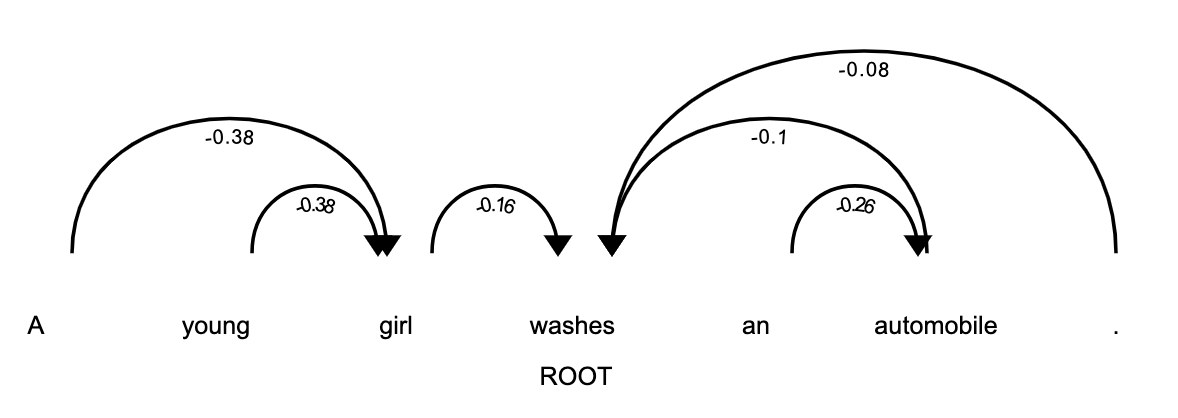
\includegraphics[width=\columnwidth]{images/all_freeze_9533.png}
        \caption{Parse obtained using the the PTB-All ($\times$) configuration.}
        \label{subfig:expl1-1}
    \end{subfigure}
    \hfill
    \begin{subfigure}[b]{0.475\textwidth}  
        \centering 
        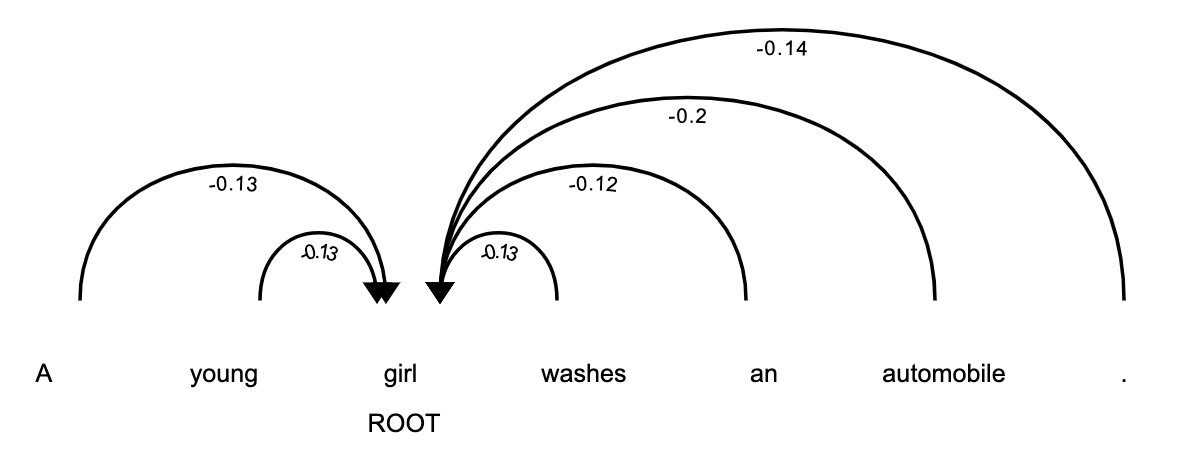
\includegraphics[width=\columnwidth]{images/all_update_9533.png}
        \caption{Parse obtained using the the PTB-All ($\checkmark$) configuration.}
        \label{subfig:expl1-2}
    \end{subfigure}
    \vskip\baselineskip
    \begin{subfigure}[b]{0.475\textwidth}   
        \centering 
        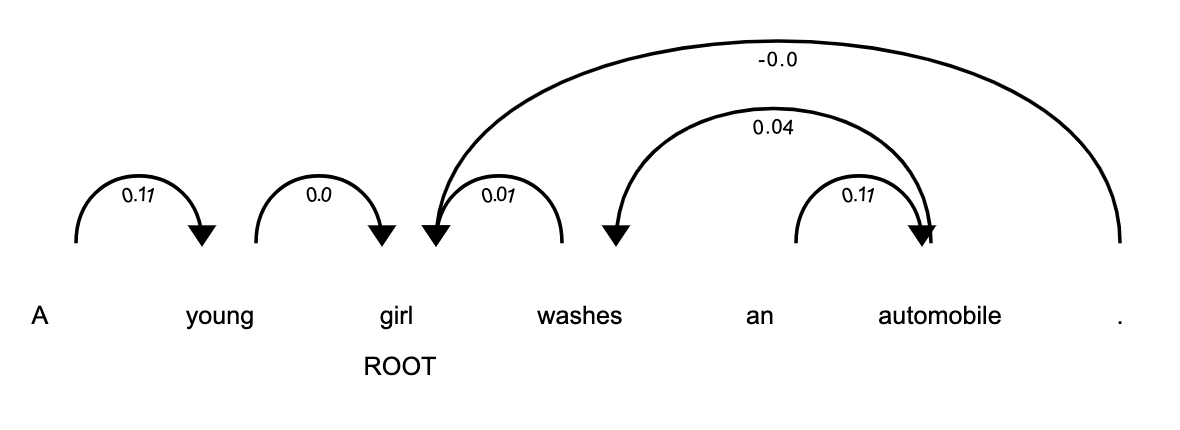
\includegraphics[width=\columnwidth]{images/100_freeze_9533.png}
        \caption{Parse obtained using the the PTB-100 ($\times$) configuration.}
        \label{subfig:expl1-3}
    \end{subfigure}
    \hfill
    \begin{subfigure}[b]{0.475\textwidth}
        \centering 
        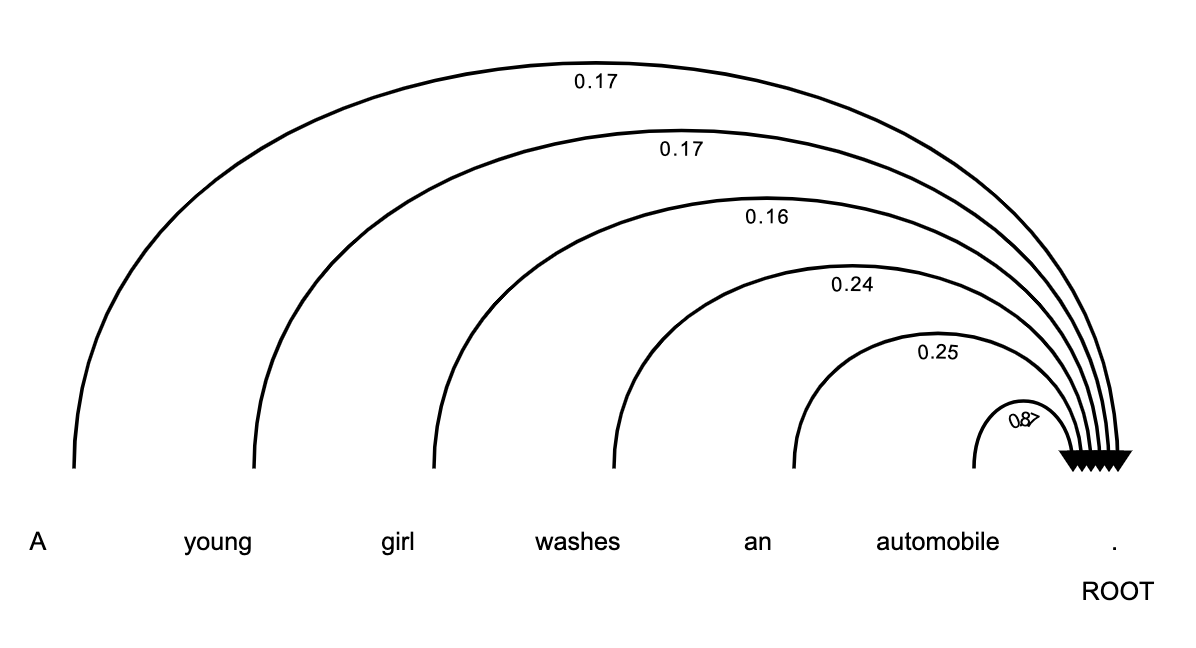
\includegraphics[width=\columnwidth]{images/100_update_9533.png}
        \caption{Parse obtained using the the PTB-100 ($\checkmark$) configuration.}
        \label{subfig:expl1-4}
    \end{subfigure}
    \vskip\baselineskip
    \begin{subfigure}[b]{0.475\textwidth}
        \centering
        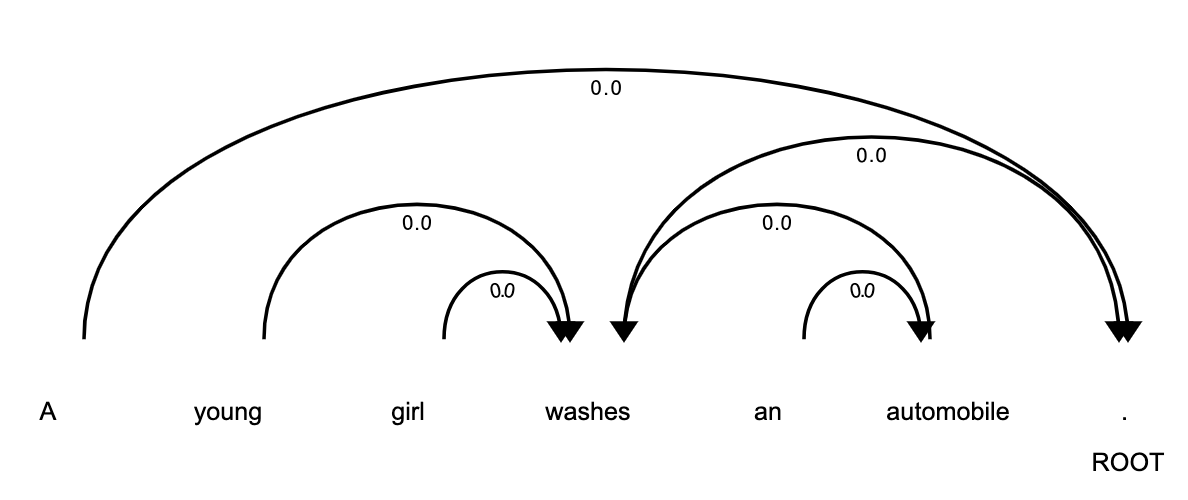
\includegraphics[width=\columnwidth]{images/bert_att_0_9533.png}
        \caption{Parse obtained using the attention head \#$1$ and without updating \textsc{Bert}.}
        \label{subfig:expl1-5}
    \end{subfigure}
    \hfill
    \begin{subfigure}[b]{0.475\textwidth}  
        \centering 
        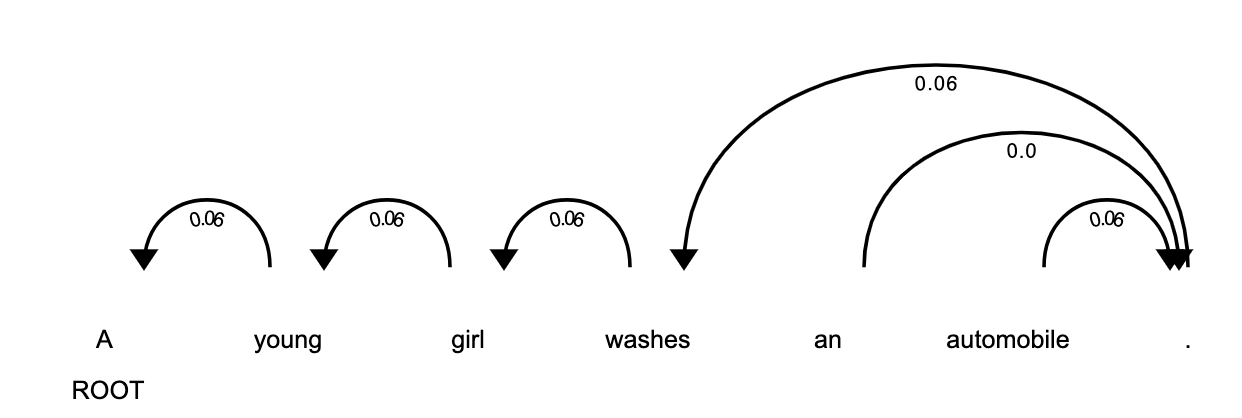
\includegraphics[width=\columnwidth]{images/bert_att_0_9533_update.png}
        \caption{Parse obtained using the attention head \#$1$ and updating \textsc{Bert}.}
        \label{subfig:expl1-6}
    \end{subfigure}
    \caption{Example of parse obtained using various configurations from our model. The parser component is initialized on PTB-All (\ref{subfig:expl1-1}, \ref{subfig:expl1-2}), PTB-100 (\ref{subfig:expl1-3}, \ref{subfig:expl1-4}) or \textsc{Bert} (\ref{subfig:expl1-5}, \ref{subfig:expl1-6}). We either freeze ($\times$) or update ($\checkmark$) the parser during the fine tuning on the SNLI. We include the weights $\alpha$ produced from the parser. 
    %We use \bert{} to obtain tree structures and evaluate the full pipeline on the \textbf{SICK-R} and \textbf{SNLI} tasks. 
    We report the accuracy from a single run on the test set.} 
    \label{fig:parse-expl}
\end{figure}

For the initialization with the PTB, we observe the fine-tuning makes the tree evolve to trivial structures and tend to connect every node to an arbitrary root. We hypothesize, such trivial structures present advantages from a computational point of view. As observed in \textcite{shi_18}, trivial trees without syntax properties might lead to surprisingly good results. \textcite{shi_18} hypothesize that trivial trees gain might benefit from shallow and balanced properties. \bcomment{un peu mystérieux ce parag}{}

For \textsc{Bert} parser initialization, we observe the fine-tuning produces rather sequential patterns, with words connected to direct neighbors. Some isolated groups of words also present inner connections.

%In our full supervised setup, we observe the parser's fine-tuning enables the model to adjust the parse from Figure~\ref{subfig:expl1-1} into the structure represented in Figure~\ref{subfig:expl1-2}. The obtained structure does match the one produced using more pre-training samples from the PTB dataset.

%In our low supervised setup, fine-tuning the parser 
%Regarding the parses obtained without any pre-training on the PTB (Figure~\ref{subfig:expl1-14), we observe all nodes tend to be connected to an arbitrarily chosen root.


%%%%%%%%%%%%%%%%%%%%%%%%%%%%%%%%%%%%%%%%%%%%%%%%%%%%%%%%%%%%%%%%%%%%%%%%%%%%%%%%%%%%%%%%
% 2. Shi
%%%%%%%%%%%%%%%%%%%%%%%%%%%%%%%%%%%%%%%%%%%%%%%%%%%%%%%%%%%%%%%%%%%%%%%%%%%%%%%%%%%%%%%%

% \textcolor{blue}{\citet{williams_18} investigate the trees produced by \citet{yogatama_17} and \citet{choi_18}. The authors show neither method produce meaningful latent trees in syntax. Moreover, Gumbel softmax outputs inconsistent latent trees across initializations while reinforcement learning outputs trivial left-branching trees. We also observe that random initialization leads to trivial trees (PTB-$\emptyset$). The PTB-100 appears as good trade off. Indeed the induced trees are close to silver references and thus meaningful regarding dependency structure. The trees are also specific to the task due to the parser fine-tuning with downstream objective.}

\subsection{Impact of the initialization on downstream tasks} % Reducing the need for annotation
\label{sec:dowstream-impact}

We observed in previous Section~\ref{sec:parses-impact} that the initialization and the training configuration of the parser component deeply impact the resulting parses. We now study the impact of the parser initialization on downstream performances.

%\paragraph{Initialization with human annotated data} % Reducing the need for annotation
% First, we consider the configurations introduced in Section~\ref{sec:parses-analysis} and study the impact of the parser initialization on downstream tasks. 

\begin{table}[!htb]
\centering
\small
\begin{tabularx}{\textwidth}{@{}Y Y | Y Y@{} }
\toprule
\textbf{PTB sample size} & \textbf{Parser fine-tuning} & \textbf{SICK-R ($r$)} & \textbf{SNLI (Acc.)} \\
\midrule
\midrule 
\multicolumn{4}{c}{\textit{Linguistic annotations}}\\
\midrule
% PTB-$\emptyset$ & $\checkmark$ & 85.6 \scriptsize{(0.6)} & 81.5 \scriptsize{(0.2)}\\
% \midrule 
% PTB-100 & $\times$  & 86.6 \scriptsize{(0.2)} & 81.9 {\scriptsize (0.3)}\\
% PTB-100 & $\checkmark$ & 86.9 \scriptsize{(0.4)} & 82.6 {\scriptsize (0.2)}\\
% \midrule
% PTB-All & $\times$  & 87.2 \scriptsize{(0.2)} & 81.9 {\scriptsize (0.6)}\\
% PTB-All & $\checkmark$ & 87.5 \scriptsize{(0.4)} & 83.0 {\scriptsize (0.2)}\\
PTB-$\emptyset$ & $\checkmark$ & 85.6 \scriptsize{(85.6)} & 84.6 \scriptsize{(85.5)}\\
\midrule 
PTB-100 & $\times$  & 86.4 \scriptsize{(86.6)} & 84.5 {\scriptsize (85.5)}\\
PTB-100 & $\checkmark$ & 86.5 \scriptsize{(86.9)} & 84.9 {\scriptsize (85.8)}\\
\midrule
PTB-All & $\times$  & 86.8 \scriptsize{(87.2)} & 85.0 {\scriptsize (85.8)}\\
PTB-All & $\checkmark$ & 87.0 \scriptsize{(87.5)} & 85.0 {\scriptsize (85.5)}\\
\midrule 
\multicolumn{4}{c}{\textit{Unsupervised parser}}\\
\midrule
% avec la taille de batch de 16
% \bert{} & $\times$  & --- & 84.4 {\scriptsize (85.3)}\\
% \bert{} & $\checkmark$ & --- & 84.1 {\scriptsize (84.5)}\\
% avec la taille de batch de 128
\textsc{Bert} & $\times$  & --- & 84.4 {\scriptsize (85.3)}\\
\textsc{Bert} & $\checkmark$ & --- & 84.6 {\scriptsize (85.1)}\\
\bottomrule
\end{tabularx}
\caption{Impact of the parser initialization on downstream task performances:  We pre-train the parser module with a given sample size from the PTB. We either freeze (\textbf{$\times$}) or update (\textbf{$\checkmark$}) the parser during the fine-tuning. We report the average score test set from 5 runs for SICK-R and 2 runs for SNLI (the score from the development set are in parentheses). We report Pearson correlation by convention as $r \times 100$.}
\label{table:parser}
\end{table}

In Table \ref{table:parser}, we compare the impact of the different initializations for both tasks. For each setup, we report the Pearson correlation on the test set of the SICK-R task and the accuracy on the test set from the SNLI task.

We either freeze the parser component or continue to update it, given the downstream loss for each initialization. Fine-tuning the parser on the task generally leads to an improvement of the downstream results. In that regard, we share the observation from other latent tree learning methods \parencite{maillard_19, choi_18}; models jointly learning the parsing and composition function outperform those with a fixed structure. 

We also observe that models using the full or partial annotated data outperform models relying on the sole downstream supervision (PTB-$\emptyset$). This observation is more clear on the SICK-R task. We previously observed that fine-tuning the parser can lead to tree structure diverging from linguistic patterns. Nonetheless, regarding the downstream performances, human annotation appears as a good initialization for our model. 

% For technical reasons, we had to limit the batch size to 16 when fine-tuning \textsc{Bert} parsing module. Therefore, the benefit from fine-tuning the parser when using \textsc{Bert} is difficult to interpret. However, 
We can observe model relying on linguistic-driven structures seems to achieve better performances. Nonetheless, the difference is thin, and we present here an average score across trees obtained from all attention heads. Therefore some attention heads might present structures as efficient as linguistic patterns.

\section{Conclusion}

Results are half in jest, half in earnest. We evaluate our model on textual entailment and semantic similarity tasks. Regarding the textual similarity task, we show that our setup is competitive with \textsc{Bert} base, although the latest is trained on datasets many orders of magnitude larger. We explore to which extend the trees produced by our model compare with linguistic structures and how this initialization impacts downstream performances. We empirically observe that downstream supervision troubles producing stable parses and preserving linguistically relevant structures.  % We corroborate that the sole use of downstream supervision is insufficient to produce parses that are easy to interpret. 
To encourage convergence towards readable linguistic structures, we examine a number of initialization setups. Depending on the optimization setup, the parse tree may present instability. We also observe that our structures often converge toward trivial branching patterns, which have few in common with gold linguistic parses. However, with respect to the downstream performances, linguistic insights appear as a relevant initialization.
\setchapterstyle{kao}
\setchapterpreamble[u]{\margintoc}
\chapter{Studying shallow structure in transformer models}
\labch{transformers}

\cleanchapterquote{At midnight in the month of June,\\
     I stand beneath the mystic moon.\\
     An opiate vapour, dewy, dim,\\
     Exhales from out her golden rim,\\
     And, softly dripping, drop by drop,\\
     Upon the quiet mountain top.\\
     Steals drowsily and musically\\
     Into the univeral valley.\\
     \textup{[\,\dots]}}{Edgar Allan Poe}{The Sleeper, 1831}

% In the previous chapter, we developed linguistically inspired tree-based models. We designed a model to reduce the need for carefully hand-annotated data. Yet, we exhibit other practical limitations of these models: structure instabilities across runs, inconsistency with linguistic insights or even convergence towards trivial branching patterns. 

% performance increment in downstream applications
\bcomment{Because of their practical constraints and limited performance increment}{generally require annotations}, the community has lost some interest in tree-structured models. In contrast, alternative methods such as recurrent neural networks \parencite{hochreiter_97, cho_14} or transformers \parencite{vaswani_17} have gained proportional popularity in recent years. Unlike tree-based models, these methods require \bcomment{only raw text as input}{not exactly : rather, these language models do not require costly annotations (LSTM etc. can be used with supervision as a building block of complex networks}. 

Transformers introduce a profound paradigm shift with recurrent and recursive architectures. For the latter, the input structure determines the computational path: recurrent networks process words sequentially given their order ; recursive networks process words in a bottom up manner—starting from the leaves, up to the root. In contrast, Transformers process all words simultaneously through a fixed number of layers and do not appear to follow a specific structure. Yet, as many results suggest \parencite{linzen_16, jawahar_19, clark_19}, these new models acquire some sort of \bcomment{tree}{text, we do not know it this is a tree} structure.

This chapter makes the parallel with transformers and sequential or tree structured models. We interpret transformers as structured neural networks and layers as operations on trivial fully connected graphs. We challenge our formalism by conducting an empirical investigation of the role of multiple layers in deep transformer models. We propose a variant of \textsc{Albert} \parencite{simoulin_2021b} that dynamically adapts the number of layers applied to each token and analyze token transformation across the network depth.

% After reviewing the related work (\refsec{transformers:dynamic-depth}), we detail the model and the training methodology in \refsec{transformers:architecture}. In particular, we encourage our model to be parsimonious and limit the total number of iterations performed on each token. In \refsec{transformers:experiments}, we analyze iterations of the model during pre-training, fine-tuning and inference. 


% In this chapter, we aim to better characterize the latent structure in transformers and provide the tools to analyze them.

% Indeed, these methods, unlike tree-based models, require only raw text as input. On the other hand, as many results suggest \parencite{linzen_16, jawahar_19, clark_19}, these new models acquire some sort of tree structure.


% Due to their practical constraints and limited improvement in downstream performance, tree-structured models have somehow lost the light from the community. been limited in their application.

% Because of their practical constraints and limited performance improvement in downstream applications, tree-structured models have lost some of their lusters.

% The community has lost some interest in tree-structured models due to their practical constraints and limited improvement in downstream performance.

% Tree-structured models have somehow gone out of fashion due to their practical limitations and limited potential for downstream performance improvement.

% In part due to their practical limitations and limited performance improvements, tree-structured models have somehow lost their luster.

% Due to their operational constraints and limited effect on downstream performance, tree-structured models have lost a bit of popularity.

% Despite their practical limitations and little improvement in downstream performance, tree-structured models have become somewhat peripheral in the community.

% These models do not fully succeed in computing meaningful semantic representation along with explicit structure.

% The previous chapter exhibit the limits of recursive neural models. From a computational perspective, such architectures may not be optimal since they require inputting the text structure as well as the raw surface form. As argued by \textcite{choi_18}, different tasks might require different hierarchical compositions of words. The composition induced by linguistic may therefore not be optimal from a computational or task oriented perspective. We proposed an original framework, for which the structure is learned jointly with the composition function. We thus reduce the need for linguistic annotations and obtain competitive results for semantic textual similarity task. Yet, the inferred structure might present some instabilities across runs, differ from linguistic insights or even converge towards trivial branching patterns.

% Tree-based models need carefully hand-annotated data to be trained. 
% \sidenote{We deep dive on the structure learned by transfomers model in \refch{transformers}.}.

% Recent transformer architectures have gained increased popularity within the community. Contrary to tree-based models, they do not need carefully hand-annotated data to be trained. On the other hand, as many results suggest, these new models acquire some sort of tree structure. 


% \section{Towards defining structure}
% \labsec{transformers:structure}


\section{Transformer as graph neural networks}

\subsection{Defining graph neural networks}

Mettre des images de graph

In this section, we summarize the graph neural network (GNN) framework as defined in \textcite{hamilton_2020}.
% \textcite{hamilton_2020} defines graph neural networks (GNN) as a framework to define neural networks on graph structured data. 
Graph neural networks operate on graph structured data. We define a graph $\mathscr{G}$ by a tuple of sets $\mathscr{G} = (\mathcal{V}, \mathcal{E})$. 
With $\mathcal{V}$ the set of vertices and $\mathcal{E}$ the set of edges between the node. 
A graph is a ubiquitous data structure that can describe many complex systems. 
For example, molecules are a group of atoms held together by chemical bonds. 
Chemical graphs are full-fledged representations of them, with vertices corresponding to atoms and edges to chemical bonds.

Graph neural networks take as input a graph $\mathscr{G}$ along with a set of node features $X \in \mathbb{R}^{d \times |\mathcal{V}|}$, with $d$ the network hidden size.
Graph neural networks generate a node embedding $z_u, \forall u \in \mathcal{V}$. They iteratively update node hidden embeddings $h_u^{k}$ using a neural message passing process. 
We can decompose each iteration in two steps: First, an \textit{aggregation} step (\refeq{aggregate}), that aggregate the information from $u$' graph neighborhood $\mathcal{N}(u)$. 
Then an \textit{update} step (\refeq{update}) that update each hidden embedding given its neighborhood aggregated information and its previous state.

\begin{align}
    m^{(k)}_{\mathcal{N}(u)} &= \mathsf{aggregate}^{(k)}\left(\{h_v^{(k)}, \forall v \in \mathcal{N}(u)\}\right), \labeq{aggregate} \\
    h^{(k+1)}_u &= \mathsf{update}^{(k)}\left(h^{(k)}_u, m^{(k)}_{\mathcal{N}(u)}\right), \labeq{update}
\end{align}

Here, the $\mathsf{aggregate}$\sidenote{The $\mathsf{aggregate}$ function takes a set as input and is therefore permutation invariant by design} and $\mathsf{update}$ function are differentiable and $m_{\mathcal{N}(u)}$ is the \textit{message} aggregated from $u$ neighborhood.

For simplification, we can add self-loops to the input graph such that $u$ is included in its own neighborhood $\mathcal{N}(u)$. 
The message passing iteration can then be defined using a single equation and we implicitly define the \textit{update} step in the \textit{aggregate} step (\refeq{update-aggregate}).

\begin{equation}
    h^{(k+1)}_u = \mathsf{aggregate}^{(k)}\left(\{h_v^{(k)}, \forall v \in \mathcal{N}(u) \cup \{u\}\}\right), \labeq{update-aggregate}\\
\end{equation}

\refeq{embeddings} defines the embedding of each node as its hidden state after $K$ message passing iterations:

\begin{equation}
    z_u = h_u^{(K)}, \forall u \in \mathcal{V}, \labeq{embeddings}\\
\end{equation}

At each iteration, each node aggregates information from its $k$-hop neighbors. Node embeddings therefore encode structural and feature based information.

\subsection{Defining transformer's message passing functions}

Transformers \parencite{vaswani_17} may easily be defined under the graph neural network framework. 
They transform inputs through a fixed number of layers.
As detailed in \refsec{training:architectures}, each layer is composed of a multi-head attention (MHA) block and a feed-forward network (FFN).
The self-attention mechanism that transforms a \textit{set of vectors} into what is known as \textit{contextualized vectors}. 
Each contextualized vector is a weighted average of the vectors from the original set.
% They operate on a set of vectors. 
Since attention compose every vector from the set, we can consider that transformers operate on fully connected graphs.
We can adapt the \refeq{update-aggregate} for transformers as follow\sidenote{In fact, we can also formally decompose transformers layers by considering the MHA layer as the $\mathsf{aggregate}$ function and the FFN layer as the $\mathsf{update}$ function. This interpretation may provide a formal background to analyze the role of the FFN.}:

\begin{align}
    h^0_u &= W_e u + W_p \labeq{update-aggregate-transformers-emb}\\
    h^{(k+1)}_u &= \text{FFN}^{(k)}\left(\text{MHA}^{(k)}\left(\{h_v^{(k)}, \forall v \in \mathcal{N}(u) \cup \{u\}\}\right) + h_v^{(k)}\right), \labeq{update-aggregate-transformers}
\end{align}

Where \refeq{update-aggregate-transformers} is the first layer: that encode words using $W_e$ embedding layer summed with positional embeddings layer $W_p$.

\subsection{Tricks and limits}

Transformers also borrow common tricks and mechanisms from graph neural networks.
As detailed in \textcite{hamilton_2020}, over-smoothing is a core issue in graph neural networks.
This issue appends when node-specific information is lost after several message passing iterations. 
In such case, the representation of every nodes tends to become very similar.
Commonly this issue is addressed by \bcomment{concatenating}{summing?} the aggregated state with the previous hidden state before performing the update state.
This skip connection aim at explicitly preserving information from the previous iteration during the update.\bcomment{preserve word identities in NLP ?}{}

Another common pitfall of graph neural networks \bcomment{is that every nodes may have a different degree}{is that nodes have different degrees}. 
This may affect the scale of the vector during aggregation.
This variance in scale may results in numerical and optimization instability. \bcomment{does it apply to transformers in NLP ?}
A common way to alleviate this issue is to normalize the operation based upon the degree of nodes involved.
The normalization is also a sensitive operations of transformers (see csordas) \bcomment{???}{sth missing here}

\bcomment{This formalization}{The transformer formalization} accounts for the linear order of words encoded in the positional embedding layer $W_p$.
\bcomment{???}{}This approach depends on the arbitrary ordering of nodes that we used in the adjacency matrix.
As a result, the approach is not permutation invariant, a standard property in traditional graph neural networks.

\subsection{Interpretation}

The formalization of transformers as graph neural networks open an original angle to interpret them.
The mechanism of transformer layers is often compared to intuitive NLP pipelines \parencite{tenney_19}. 
Starting with the lower layers encoding surface information, middle layers encoding syntax and higher layers encoding semantics \parencite{jawahar_19, peters_18}.

In the graph neural network perspective, transformers progressively refine the feature through an iterative \bcomment{message passing}{} process.
As described in \textcite{xin_20}.  become more fine-grained at each iteration.
This also provide a new interpretation path for \textsc{Albert} \parencite{lan_20}.
The model is based on the transformer architecture, except that weights are tied across layers.
From a graph neural network perspective, the model use the same message passing function at each iteration.

\subsection{Graphs, trees, sequences}
\labsec{transformers:graph}

It is also possible to extend the use of the graph neural network formalism for other NLP models.
Tree-structured models operate on tree, which are directed acyclic graph.
The Tree-LSTM equations are detailed in \refsec{training:architectures}. 
They may also be formatted in a $\text{aggregate}$ and $\text{update}$ functions.
In this case, the $\text{aggregate}$ function consists on the simple sum of the node neighborhood hidden states.
A key aspect is also that the graph defined by Tree-LSTM do not contain any loop.
the message passes in a bottom-up manner, starting from the leaf, all the way to the root.
In this case, there is only a single message passing iteration. \bcomment{why ? you might actually iterate ?}{even if probably useless}

Sequential LSTM may also be considered a particular kind of graph neural network. 
A sequence is indeed equivalent to an unary directed acyclic graph.
As for the \textsc{Tree-LSTM}, the \textsc{LSTM} equations may also be separated in a $\text{aggregate}$ and $\text{update}$ functions.
In this case the $\text{aggregate}$ function is just the identity function, since each node as exactly one children.
As for the \textsc{Tree-LSTM}, there is only a single message passing iteration.

\subsection{Are transformers over-parametrized?}

Il faut parler du pruning qui justifie que graph dense pas forcement nécessaire !! Sauf pour ettinger et distill bert

\bcomment{}{In the light of our GNN analysis\ldots transformers should naturally share parameters across layers\ldots}

It is looking like the answer is included in the question. 
Transformers are indeed admittedly over-parametrized in the litterature \parencite{chen_20, hou_20, voita_19}. 
Yet the role of this over-parametrization is not well understood. 
Transformers layers are suspected to be highly redundant \parencite{liu_20} and to cause over-fitting \parencite{fan_20, zhou_20b}. 

\bcomment{unsure what is your point here}{}We illustrate the input structure corresponding to the different architectures in \reffig{structure}.
Sequential \textsc{RNN} or \textsc{TreeRNN} operate on sparse graph data.
The number of node $|\mathcal{V}|$ is the same order of magnitude to the number of edges $|\mathcal{E}|$.
On the contrary, transformer operate on a fully connected graph. 
The number of number of edges $|\mathcal{E}|$ is equalt to the number of nodes squared $|\mathcal{V}|^2$.

Another point of comparison between these methods is the number of message passing updates.
Tree and sequences do not require multiple message passing iteration since they do not include any loop \bcomment{well\ldots }{ yes and no ?}.
Transformers are fully connected. Node hidden states cannot be computed in a given hierarchical order since they all depend from each others.
Yet, many studies show that the weighted graph form by attention weights are not homogeneous.
Many pattern may be identified in the flow of information.
We hypothesize that node hidden states will eventually converge toward a \bcomment{stable}{fix} point\bcomment{there are references in the literature}{@see https://arxiv.org/pdf/1812.08434.pdf , section 3.2}.
We also hypothesize that some nodes require more iterations than others and that this convergence process will depend from the word and its context.


% As observed in \labsec{sec:parses-impact}, these tree might have little in common

% In this Section, we aim at better defining and characterizing the notion of structure for data and computations\sidenote{\textcite{battaglia_2018} argue that "combinatorial generalization must be a top priority for AI to achieve human-like abilities, and that structured representations and computations are key to realizing this objective.".}.

% \subsection{Structured neural networks} 

% \bcomment{this section is messy}{what is your point, the computation graph is not the key abstraction, that's the message passing (see below)}

% Artificial neural networks consist of connected units called neurons. Neurons define a vector space transformation based on linear algebra operators and nonlinear activation functions. Neural networks typically contain a very large number of neurons, which may be arranged into layers. Neurons—and by extension layers—are inter-connected: they receive input from their inner connections and send their output to their outer connections. Each layer has its own inner structure and connection pattern. The collection of layers and their connections forms a directed \textit{computational graph}. 
% Feed forward networks produce a directed acyclic computational graph. But Recurrent networks allow for connection between the same or previous layer, thus introducing cycles in the computational graph.

% Static neural networks have a fixed computational graph. In such case, inputs are all formatted according to a given standard, for instance images with $64 \times 64$ pixels. While the inputs numerically differ, they all follow the same sequence of transformation across layers. Other networks (such as the \textsc{LSTM} and \textsc{TreeLSTM} introduced in \refch{tree}) process inputs with variable format. In this case, the computational graph varies for each input sample\sidenote{We refer to such architectures as dynamic networks \parencite{han_2021}.}. Sequential recurrent networks operate with sequences as input, tree recurrent networks with trees. Sequences and trees induce a notion of hierarchy. We can assign: an index to each element in a sequence, based on their order~; a depth to each element in a tree, based on the length of the shortest path to the root node. This hierarchy directly impacts the computational order of the corresponding architectures. For recurrent or recursive neural networks, the computational graph follows the topological structure of the input, respectively a sequence or a tree.

% Sequential recurrent networks process words sequentially given their order. Tree recurrent networks process words in a bottom up manner: starting from the leaves, up to the root.
% Transformers operate on fixed length input and apparently \bcomment{fall on the static network category}{nope, the computation graph is different for sentences with different lengths (in theory), same computation is practical}. As \textcite{hamilton_2020, joshi_2020}, we argue in the next section that we may interpret transformers as a structured network operating on fully connected directional graph.
% We refer to intermediate layer outputs as hidden states. 

% Neural networks process samples trough the layers, along with the computational graph. We refer to intermediate layer outputs as hidden states. The hidden states consist of latent distributed representations. They are not design such that their coordinates reflect some specific semantic information. Yet, for the architectures introduced in \refsec{training:architectures} (\textsc{LSTM}, \textsc{TreeLSTM}, or transformers) it is possible to associate the hidden states $h_t$ to a specific word $w_t$ from the input sequence.

% We refer to the graph defined by the collection of layers and their connections as the network structure. If the network structure is a directed acyclic graph, we refer to the model as a feed forward network. If the network structure allow connection between the same or previous layer, we called it a recurrent network. Finally, recursive neural networks allow connection if the form of a given tree topological order. 

% Interestingly, the network structure may be defined regarding the input structure...

% Artificial neural networks are a collection of connected units called neurons. Neurons are connected to each others in various patterns. The network of the neurons and their inner connection forms a directed, weighted graph.

% Since their introduction, deep learning models have strongly evolve. While, in theory, they could express any function using a sole MLP layer. In practise, Their architectures evolve and overcome their practical constraints. Such as gradient overflow. In recent architectures, we introduce inductive biases. and not dense connection. We can interperet these choosen connections using graphical models.

% Structure is not a well define notion.
% It can points to the inherent structure of the input. For examples, molecules have a structure describe by their atoms and the link between them. 

% This structure can be more fuzzy. Some atoms links are differents and less trong than others. Language is often describe using a recursive tree structure and several formalism exists. Images may also be describe by meta elements and the link between them.

% This structure is also different from the model structure use to encode the elemnts. For example, molecule can be encoded using a sequential recurrent networks, relying on a sequential structure. But some mechanisms may help to account for the recursive structure such as memomry cell (c.f. eaxmples verbs subject agreement)

% In this section we aim at precisely defining the notion of structure.

% We define the input of the input as a set of elements $W$ and a set of relations between them $S$.

% We define the structure of the model as the element and the computational order in which their are computed. (pas exactement ça putot définition enf contion des entrée sorties).

% \subsection{Graph Structure} 

% \bcomment{potential structure for the whole beginning of chapter}{
% Providing a clear view on transformers would be real plus value of this chapter (insightful for many readers). It is worthwhile to spend time on it. Start with Graph neural networks (abstract graph based presentation, see Hamilton):
% \begin{enumerate}
% \item State that you analyze transformers as a GNN with message passing between the node embeddings of the GRAPH (Hamilton). And provide a schema or two like Hamilton\\
% \item It entails that transformers are iterative, it explains there are many layers
% \item State that the heads and the feedforward connections are part of the extra stuff + the parametrization of each layer + positional embeddings 
% \item Once it is done. Explain that in the case of language and with transformers the graph considered is fully connected.
% \item Then and only then, explain that you can compare the message passing behavior of transformers to the message passing behavior of the other models (your plots in Fig 5.1 are insightful bc they show the extra connectivity of transformers.
% \item You might also stress that transformers do iterative refinements while other models (LSTMSs) do not. Yet, how does the message passing looks like with stacked LSTMs ?
% \end{enumerate}
% To summarize, do not mess up with the computation graph, but rather take advantage of the message passing framework of Hamilton
% }


% \bcomment{I disagree with some of your plots}{for the LSTM plots, I would add (or at least mention) indirect arcs that connect each word to ALL its predecessors, same for tree LSTMs}

% % Many data exhibit an explicit structure. 
% We define a graph $\mathscr{G}$ by a tuple of sets $\mathscr{G} = (\mathcal{V}, \mathcal{E})$. With $\mathcal{V}$ the set of vertices and $\mathcal{E}$ the set of edges between the node. A graph is a ubiquitous data structure that can describe many complex systems. For example, molecules are a group of atoms held together by chemical bonds. Chemical graphs are full-fledged representations of them, with vertices corresponding to atoms and edges to chemical bonds.

% \begin{table}[!htb]
%   \small
%   \centering {
%   \begin{tabularx}{\textwidth}{YYYc}
%     \toprule
%     \textbf{Architecture} & \textbf{Data structure} & $\mathcal{V}$ & $\mathcal{E}$\\
%     \midrule
%     \textsc{LSTM} & Sequence & $\{w_i\}_{i \in \llbracket 1, N \rrbracket}$ & $\{(w_i, w_{i+1})\}_{i \in \llbracket 1, N \rrbracket}$\\
%     Childsum \textsc{TreeLSTM} & Tree & $\{w_i\}_{i \in \llbracket 1, N \rrbracket}$ & $\{(w_i, w_{j})\}_{i \in \llbracket 1, N \rrbracket, j \in C(i)}$\\
%     Nary \textsc{TreeLSTM} & Tree & $\{w_i\}_{i \in \llbracket 1, N \rrbracket} + \{c_i\}_{i \in \llbracket 1, M \rrbracket}$ &  $\{(w_i, w_{j})\}_{i \in \llbracket 1, N \rrbracket, j \in C(i)}$\\
%     Transformer & Graph & $\{sw_i\}_{i \in \llbracket 1, N \rrbracket}$ & $\{(sw_i, sw_{j})\}_{i, j \in \llbracket 1, N \rrbracket}$ \\
%     \bottomrule
%   \end{tabularx}}
%   \caption{For each sentence encoder architecture, we pair a sentence data structure. We formalize each structure as a specific graph. We describe sequences as unary directed acyclic graph and tree as directed acyclic graph. We associate transformers to fully connected directed graph as argued in \refsec{transformers:structure}. We notations defined in \refsec{training:architectures}: $w$ corresponds to a word and $sw$ to a subwords. $c$ are consitutents. $C(j)$ denote the set of children of node $j$.}
%   \labtab{graph-structure}
% \end{table}

% Regarding language, we can decompose a sentence using the linear order of words. In this case, we represent the sentence by an \textit{ordered sequence} of words $W = (w_1, w_2, \cdots, w_N)$. An equivalent formalism will be to represent the sentence as a \textit{set} of words $\mathcal{V} = \{w_1, w_2, \cdots, w_N\}$ and a set of relations between them $\mathcal{E} =\{(w_i, w_{i+1})\}_{i=1 \cdots N}$. In \reftab{graph-structure}, we formalize the input structure of \textsc{LSTM}, Childsum \textsc{TreeLSTM} and Nary \textsc{TreeLSTM} as graphs.

% % Dependency parsing describe the sentence as a tree for which each node corresponds to a sentence word and each vertex corresponds to a relation between two words. Formally, the sentence can still be described as as a \textit{set} of words $W$ and a set of relations between them $S$. However, in such case, the set of relations will describe a tree. Finally, constituency parsing describes the sentence as a tree. Except, intermediary nodes are used. We can still use the same formalism but we need to include intermediate consituents in the definition: a \textit{set} of words and constituents $W = \{w_1, w_2, \cdots, w_N, c_1, c_2, \cdots, c_M\}$.

% \subsection{Transformers as graph neural networks}
% \labsec{transformers:structure}

\begin{figure}[htb!]
    \centering
    \begin{subfigure}[b]{0.475\textwidth}
        \centering
        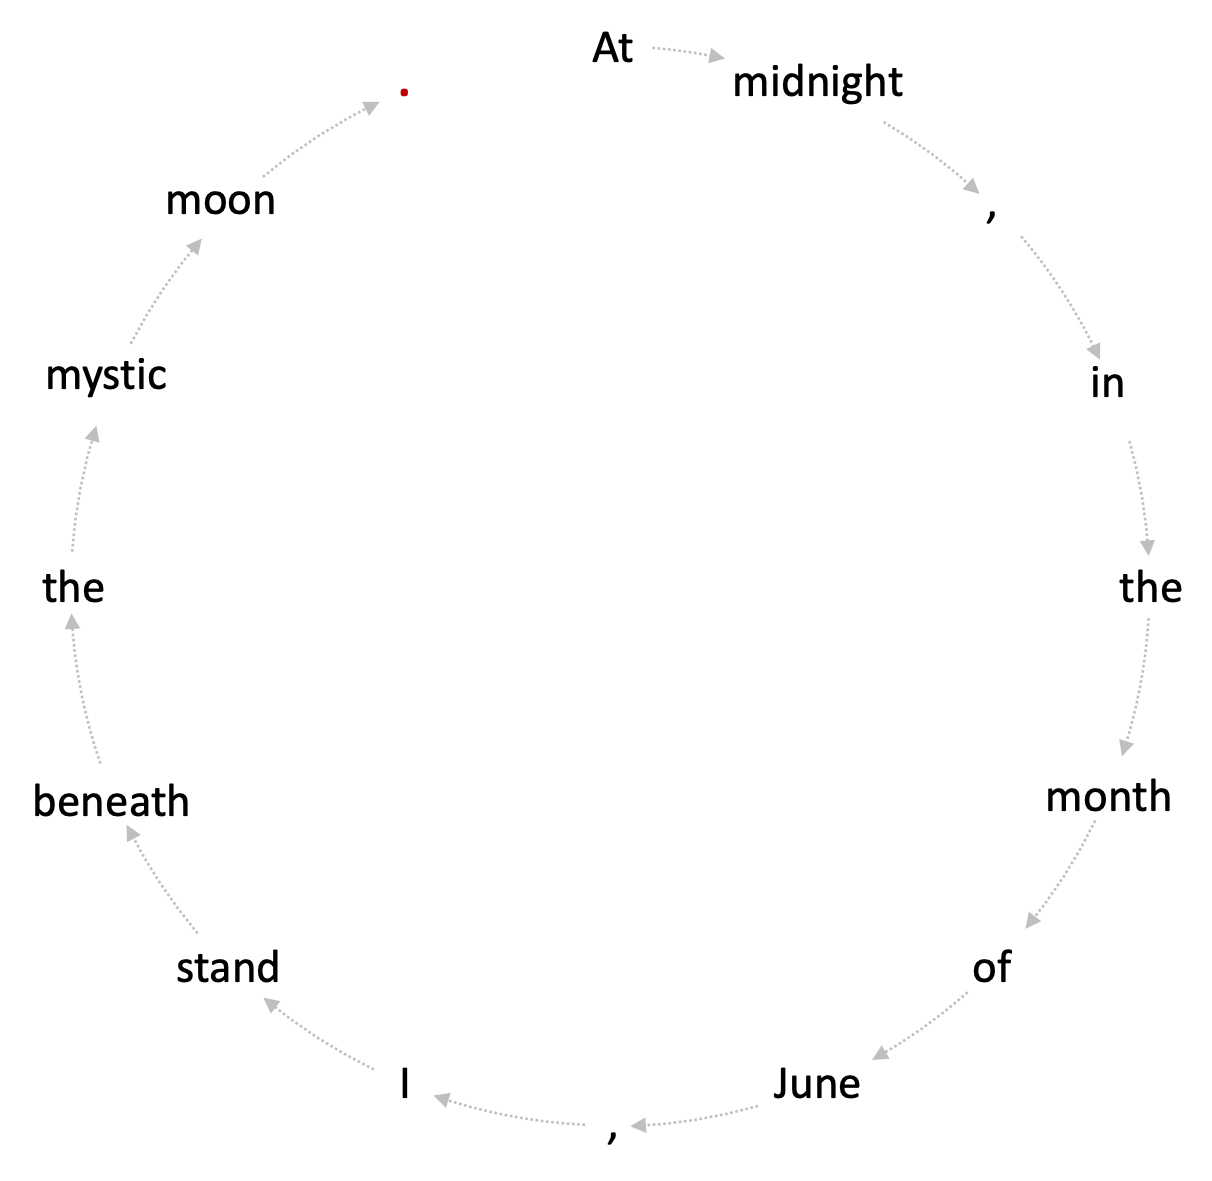
\includegraphics[width=\columnwidth]{images/rnn_uni.png}
        \caption{Unidirectional RNN}
        \labfig{subfig:structure-1}
    \end{subfigure}
    \hfill
    \begin{subfigure}[b]{0.475\textwidth}  
        \centering 
        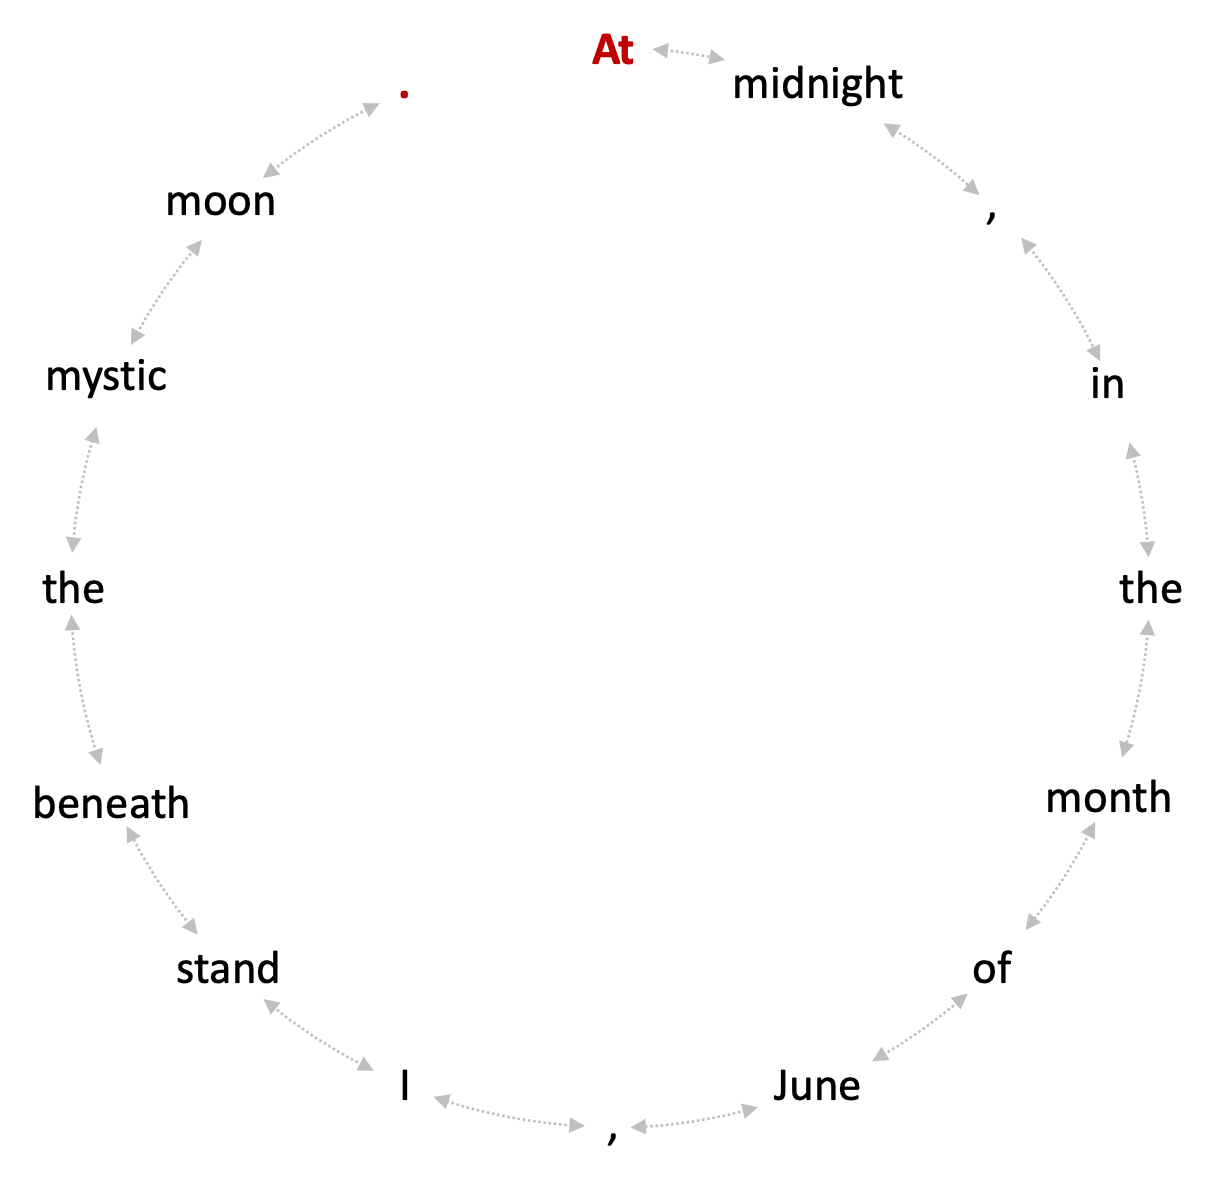
\includegraphics[width=\columnwidth]{images/rnn_bi.png}
        \caption{Bidirectional RNN}
        \labfig{subfig:structure-2}
    \end{subfigure}
    \vskip\baselineskip
    \begin{subfigure}[b]{0.475\textwidth}   
        \centering 
        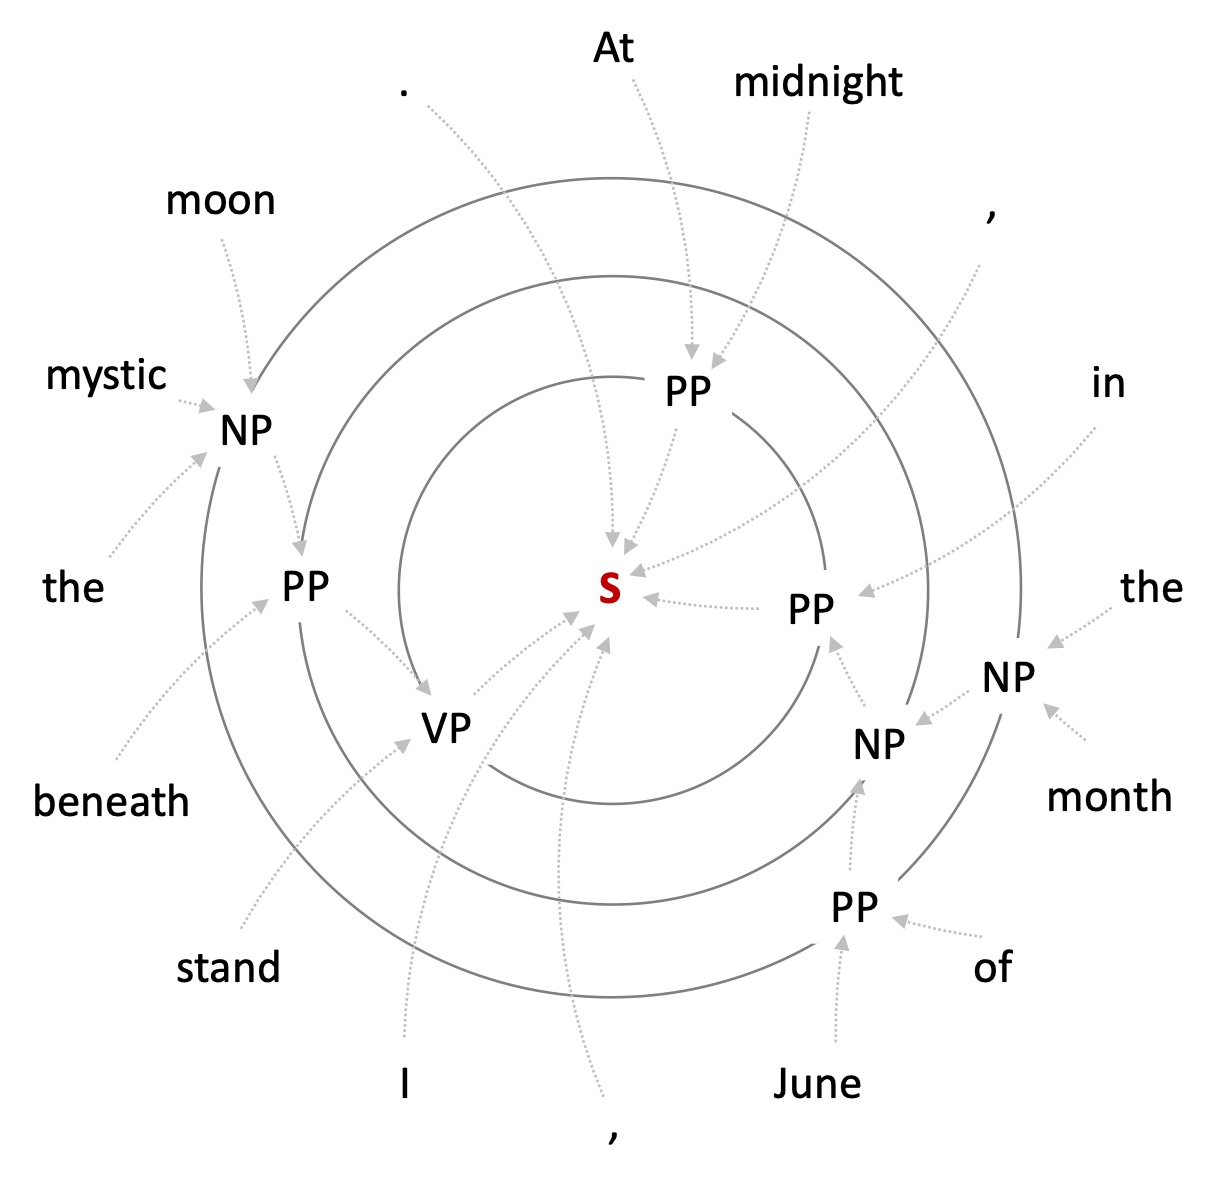
\includegraphics[width=\columnwidth]{images/rnn_const.png}
        \caption{N-ary Tree RNN}
        \labfig{subfig:structure-3}
    \end{subfigure}
    \hfill
    \begin{subfigure}[b]{0.475\textwidth}
        \centering 
        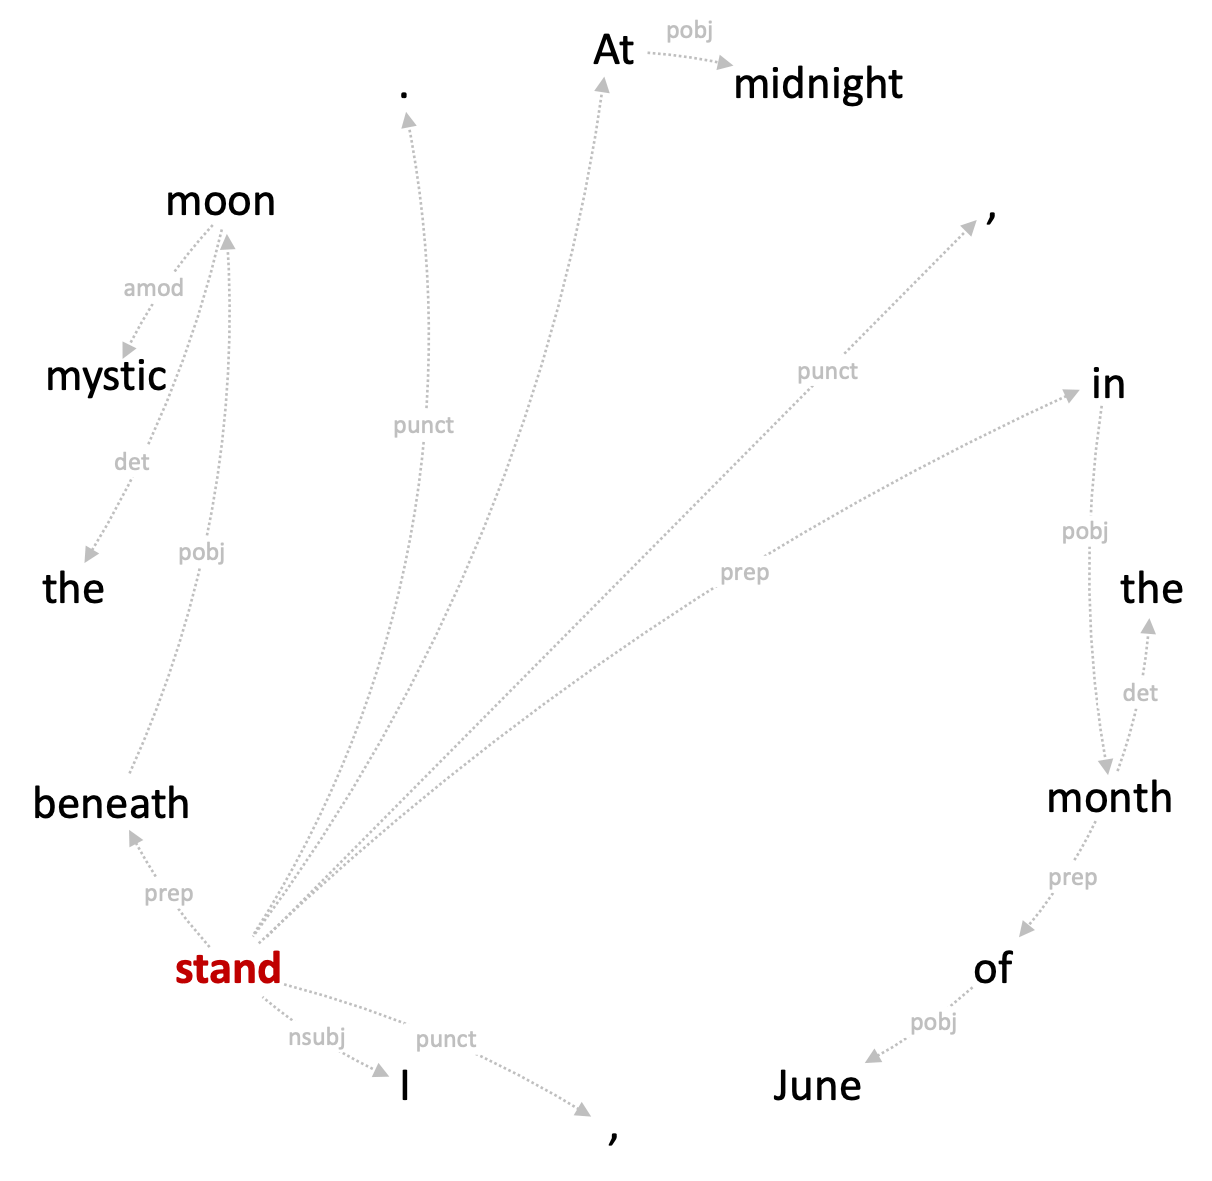
\includegraphics[width=\columnwidth]{images/rnn_dep.png}
        \caption{Childsum Tree RNN}
        \labfig{subfig:structure-4}
    \end{subfigure}
    \vskip\baselineskip
    \begin{subfigure}[b]{0.475\textwidth}
        \centering
        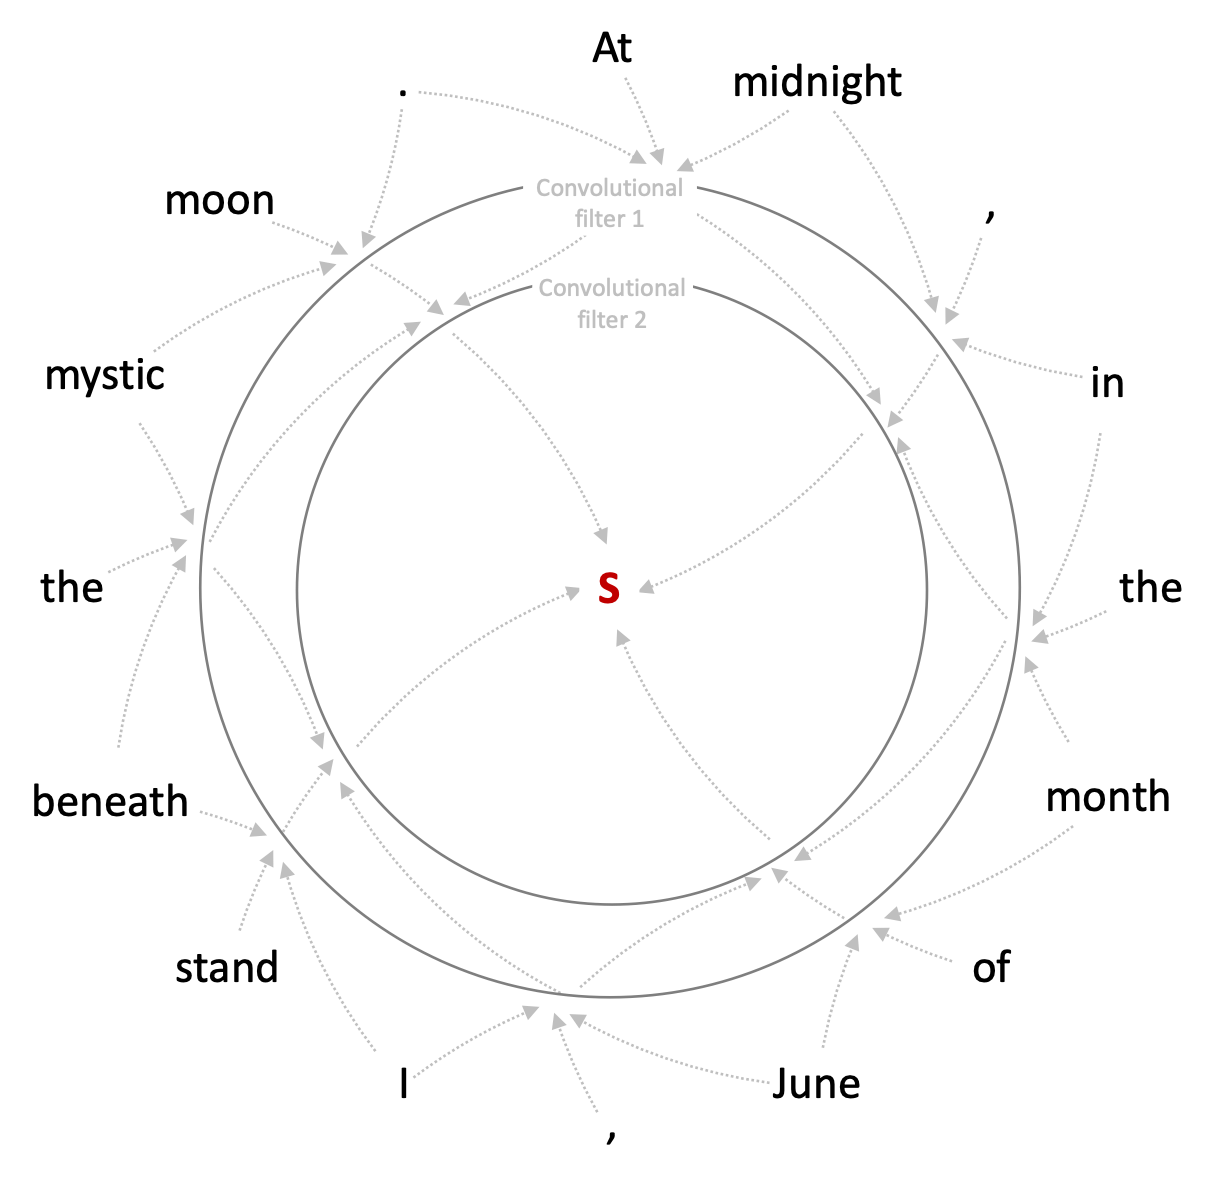
\includegraphics[width=\columnwidth]{images/conv.png}
        \caption{Convolutional NN}
        \labfig{subfig:structure-5}
    \end{subfigure}
    \hfill
    \begin{subfigure}[b]{0.475\textwidth}  
        \centering 
        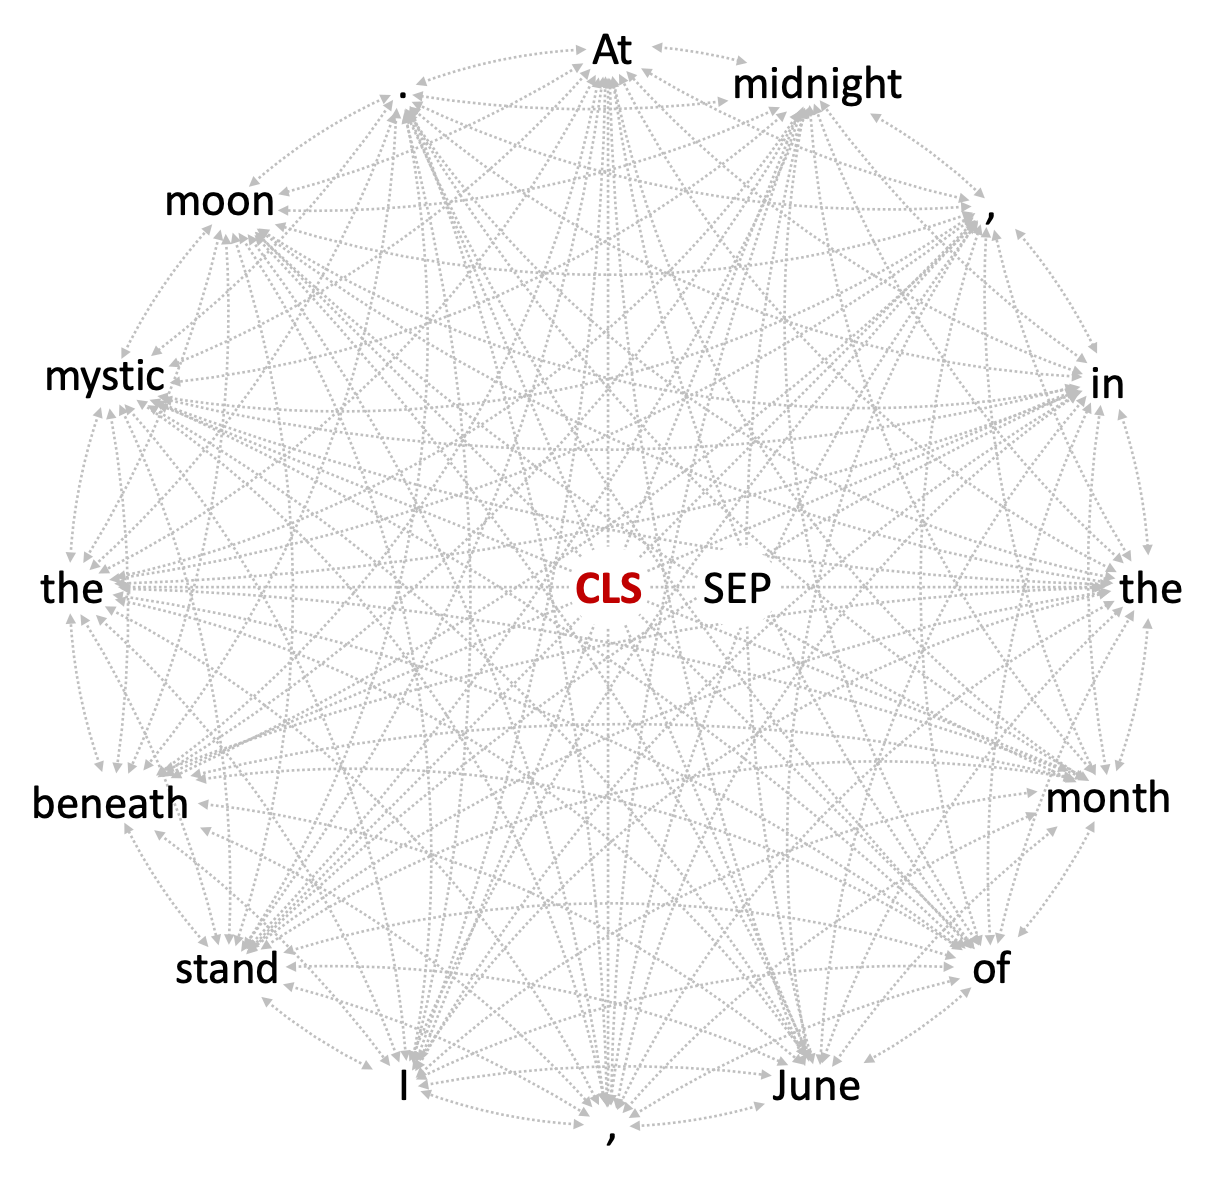
\includegraphics[width=\columnwidth]{images/transformer.png}
        \caption{Transformer NN}
        \label{subfig:structure-6}
    \end{subfigure}
    \caption{Latent structure for distinct standard NLP architectures. Illustration on the first line of the poem: "The Sleeper" by Edgar Allan Poe (published 1831). We obtain the constituency tree for \reffig{subfig:structure-3} using Berkley neural parser \parencite{klein_18}. For \reffig{subfig:structure-4}, we parse the sentence using the dependency parser from Spacy (\url{https://spacy.io/api/dependencyparser}) \parencite{honnibal_15}.} 
    \labfig{structure}
\end{figure}

% % Transformers introduce a deep paradigm shift in NLP neural architectures. 
% Transformers rely on self-attention: a mechanism that transforms a \textit{set of vectors} into what is known as \textit{contextualized vectors}. Each contextualized vector is a weighted average of the vectors from the original set. This mechanism induces a relation between every token from the input. Formally, the set of tokens and their inner relations describes a fully connected directed graph. We illustrate the input structure corresponding to the different architectures in \reffig{structure}.

% % We argue that the underlying structure for transformers is a graph. Since their is an alignment between model and data structure.

% \bcomment{additional comments}{you might also state that parsers (child sum tree LSTM here, for N-ary they introduce extra nodes) do select a particular spanning tree over the transformer fully connected graph}

% \section{Analyzing transformers shallow structure}

% In this paper we provide a study on the role of the multiple layers traditionally used. 

% The mechanism of transformer layers is often compared to intuitive NLP pipelines \parencite{tenney_19}. Starting with the lower layers encoding surface information, middle layers encoding syntax and higher layers encoding semantics \parencite{jawahar_19, peters_18}. Transformers progressively refine the features, which become more fine-grained at each iteration \parencite{xin_20}.  However, \textsc{Albert}  \parencite{lan_20} highlights that it is possible to tie weights across layers and repeat the application of the same function. Consequently, we hypothesize that it is the number of layer applications that gradually abstracts the surface information into semantic knowledge.
% % We do not fully understand the role of layers and how they process information.

% % We make the hypothesis that, the distinct layers do not encode specific surface, syntactic nor semantic functions but such information emerges through the iterative application of layers. 
% % that the layer itself may not carry specific linguistic functions. 


% \bcomment{problematize}{given the iterative behavior of transformer state that you are interested to figure out if some words would benefit from receiving more messages than others (and what is the dynamic) and if so do these words have specific hierarchical properties}

% To better study the transformation of token representations across layers, we propose a variant of \textsc{Albert} . Our model implements the key specificity of weights tying across layers but also dynamically adapts the number of layers applied to each token. Since all layers share the same weight, we refer to the application of the layer to the hidden states as an \textit{iteration}. 
% % We interpret the repetitive application of the same layer to the input as an iterative process. 

\section{Dynamic transformer depth}
\labsec{transformers:dynamic-depth}
\bcomment{After reading the whole chapter we critically miss here the research hypothesis and a plan of the remaining of the chapter}
\bcomment{State your problem immediately and provide your hypothesis}{then refs to the literature} Adapting the transformer depth is an active subject of research. In particular, deep transformer models are suspected to struggle to adapt to different levels of difficulty. While large models correctly predict difficult examples, they over-calculate simpler inputs \parencite{liu_20}. This issue can be addressed using \textit{early-stopping}: some samples might be sufficiently simple to classify using \bcomment{intermediate}{shallow ?} features. 

Some models couple a classifier to each layer \parencite{zhou_20b, liu_20, xin_20}. After each layer, given the classifier output, the model either immediately returns the output or passes the sample to the next layer. 
Exiting too late may even have negative impacts due to the network "over-thinking" the input \parencite{kaya_19}. 

Ongoing research also refines the application of layers at the token level. \textcite{wang_20} build sentence embeddings by combining token representations from distinct layers. \textcite{elbayad_20} and \textcite{dehghani_19} successfully use dynamic layers depth at the token level for full transformers (encoder-decoder). However, to the best of our knowledge, our attempt is the first to apply such mechanism to encoder only transformers and to provide an analysis of the process. 

% \section{Method}

\subsection{Model architecture}
\labsec{transformers:architecture}

In this Section, we detail the model architecture, illustrated in \reffig{transformers:model}, and pre-training procedure.
% \sidenote{We give experimental details in Appendix~\ref{appendix:datum-infra}.}.

We use a multi-layer transformer encoder \parencite{devlin_19} which transforms a context vector of tokens $(u_1 \cdots u_{T})$ through a stack of $L$ transformer encoder layers (Eq. \ref{eq:first-layer}, \ref{eq:layers}). 
% All $\mathsf{layer}_{i \in [1, n]}$ applies multi-headed self-attention follow by a position-wise feedforward operation. 
We use weight tying across layers and apply the same transformation function at each iteration \parencite{lan_20}.

\begin{align}
    h^0_t &= W_eu_t + W_p \label{eq:first-layer}\\
    h^n_t &= \mathsf{layer}(h^{n-1}_t) \quad \forall n \in [1, L] \label{eq:layers}
\end{align}

For the first layer, $W_e$ is the token embedding matrix, and $W_p$ the position embedding matrix. 

We augment the model with a halting mechanism, which allows dynamically adjusting the number of \bcomment{layers}{iterations} for each token (Eq. \ref{eq:halting-1} to \ref{eq:ponder-loss}). We directly adapted this mechanism from \textcite{graves_16}. The main distinction with the original version is the use of a transformer model instead of a recurrent state transition model. The mechanism works as follow: at each iteration $n$, we add the following operations after Eq.~\ref{eq:layers}. We assign a probability to stop $p^n_t$ for each token at index $t$ (Eq.~\ref{eq:halting-1}). 
% These probabilities are summed across layers and increase at each step. 
Given this probability, we compute an update weight $\lambda^n_t$ (Eq.~\ref{eq:halting-22}), which we use to compute the final state as the linear convex combination between the previous and current hidden state (Eq.~\ref{eq:halting-3}). 


\begin{align}
    % s^n_t &= \mathsf{layer}(h^{n-1}_t) \label{eq:halting-1}\\
    p^n_t &= \sigma\left(W_hh^n_t+b_n\right) \label{eq:halting-1}\\
    %\lambda^n_t &= R_t^n \text{ if } R_t^n \geq \epsilon \text{ else } 0 \label{eq:halting-2}\\
    \lambda^n_t &=  p^n_t \text{ if } n < N_t, R_t \text{ elif } n = N_t, \text{ else } 0 \label{eq:halting-22}\\
    % \lambda^n_t &= R_t^n \text{ if } n \leq N_t \text{ else } 0 \label{eq:halting-22}\\
    h^n_t &= \lambda^n_th^n_t + (1-\lambda^n_t)h^{n-1}_t \label{eq:halting-3}
\end{align}

With $\sigma$ the sigmoid function. We define the remainder $R_t$ and the number of iterations for the token at index $t$, $N_t$ with:

%With $R_t^n$ defined such that:
\begin{equation}
R_t=1-\sum_{l=1}^{N_t-1}p^l_t. ~~~~~N_{t}=\min_{n^{\prime}}\sum_{n=1}^{n^{\prime}}p^n_t \geq 1-\epsilon \label{eq:halting-r}
% R_t^n=1-\sum_{l=1}^{n}p^l_t. ~~~~~N_{t}=\min_{n^{\prime}}\sum_{n=1}^{n^{\prime}}p^n_t \geq 1-\epsilon \label{eq:halting-r}
%R_t^n=1-\sum_{l=1}^{n}p^l_t%. ~~~~~N_{t}=\min_{n^{\prime}} R_t^{n^{\prime}} < \epsilon
\end{equation}

% The update weights $\lambda^n_t$ decrease at each iteration. 
As soon as the sum of the probability becomes greater than $1$, the update weights $\lambda^n_t$ are set to 0 and the token is not updated anymore (Eq.~\ref{eq:halting-22}). A small $\epsilon$ factor ensures that the network can stop after the first iteration (Eq.~\ref{eq:halting-r}).

\begin{figure}[!htb]
\begin{center}
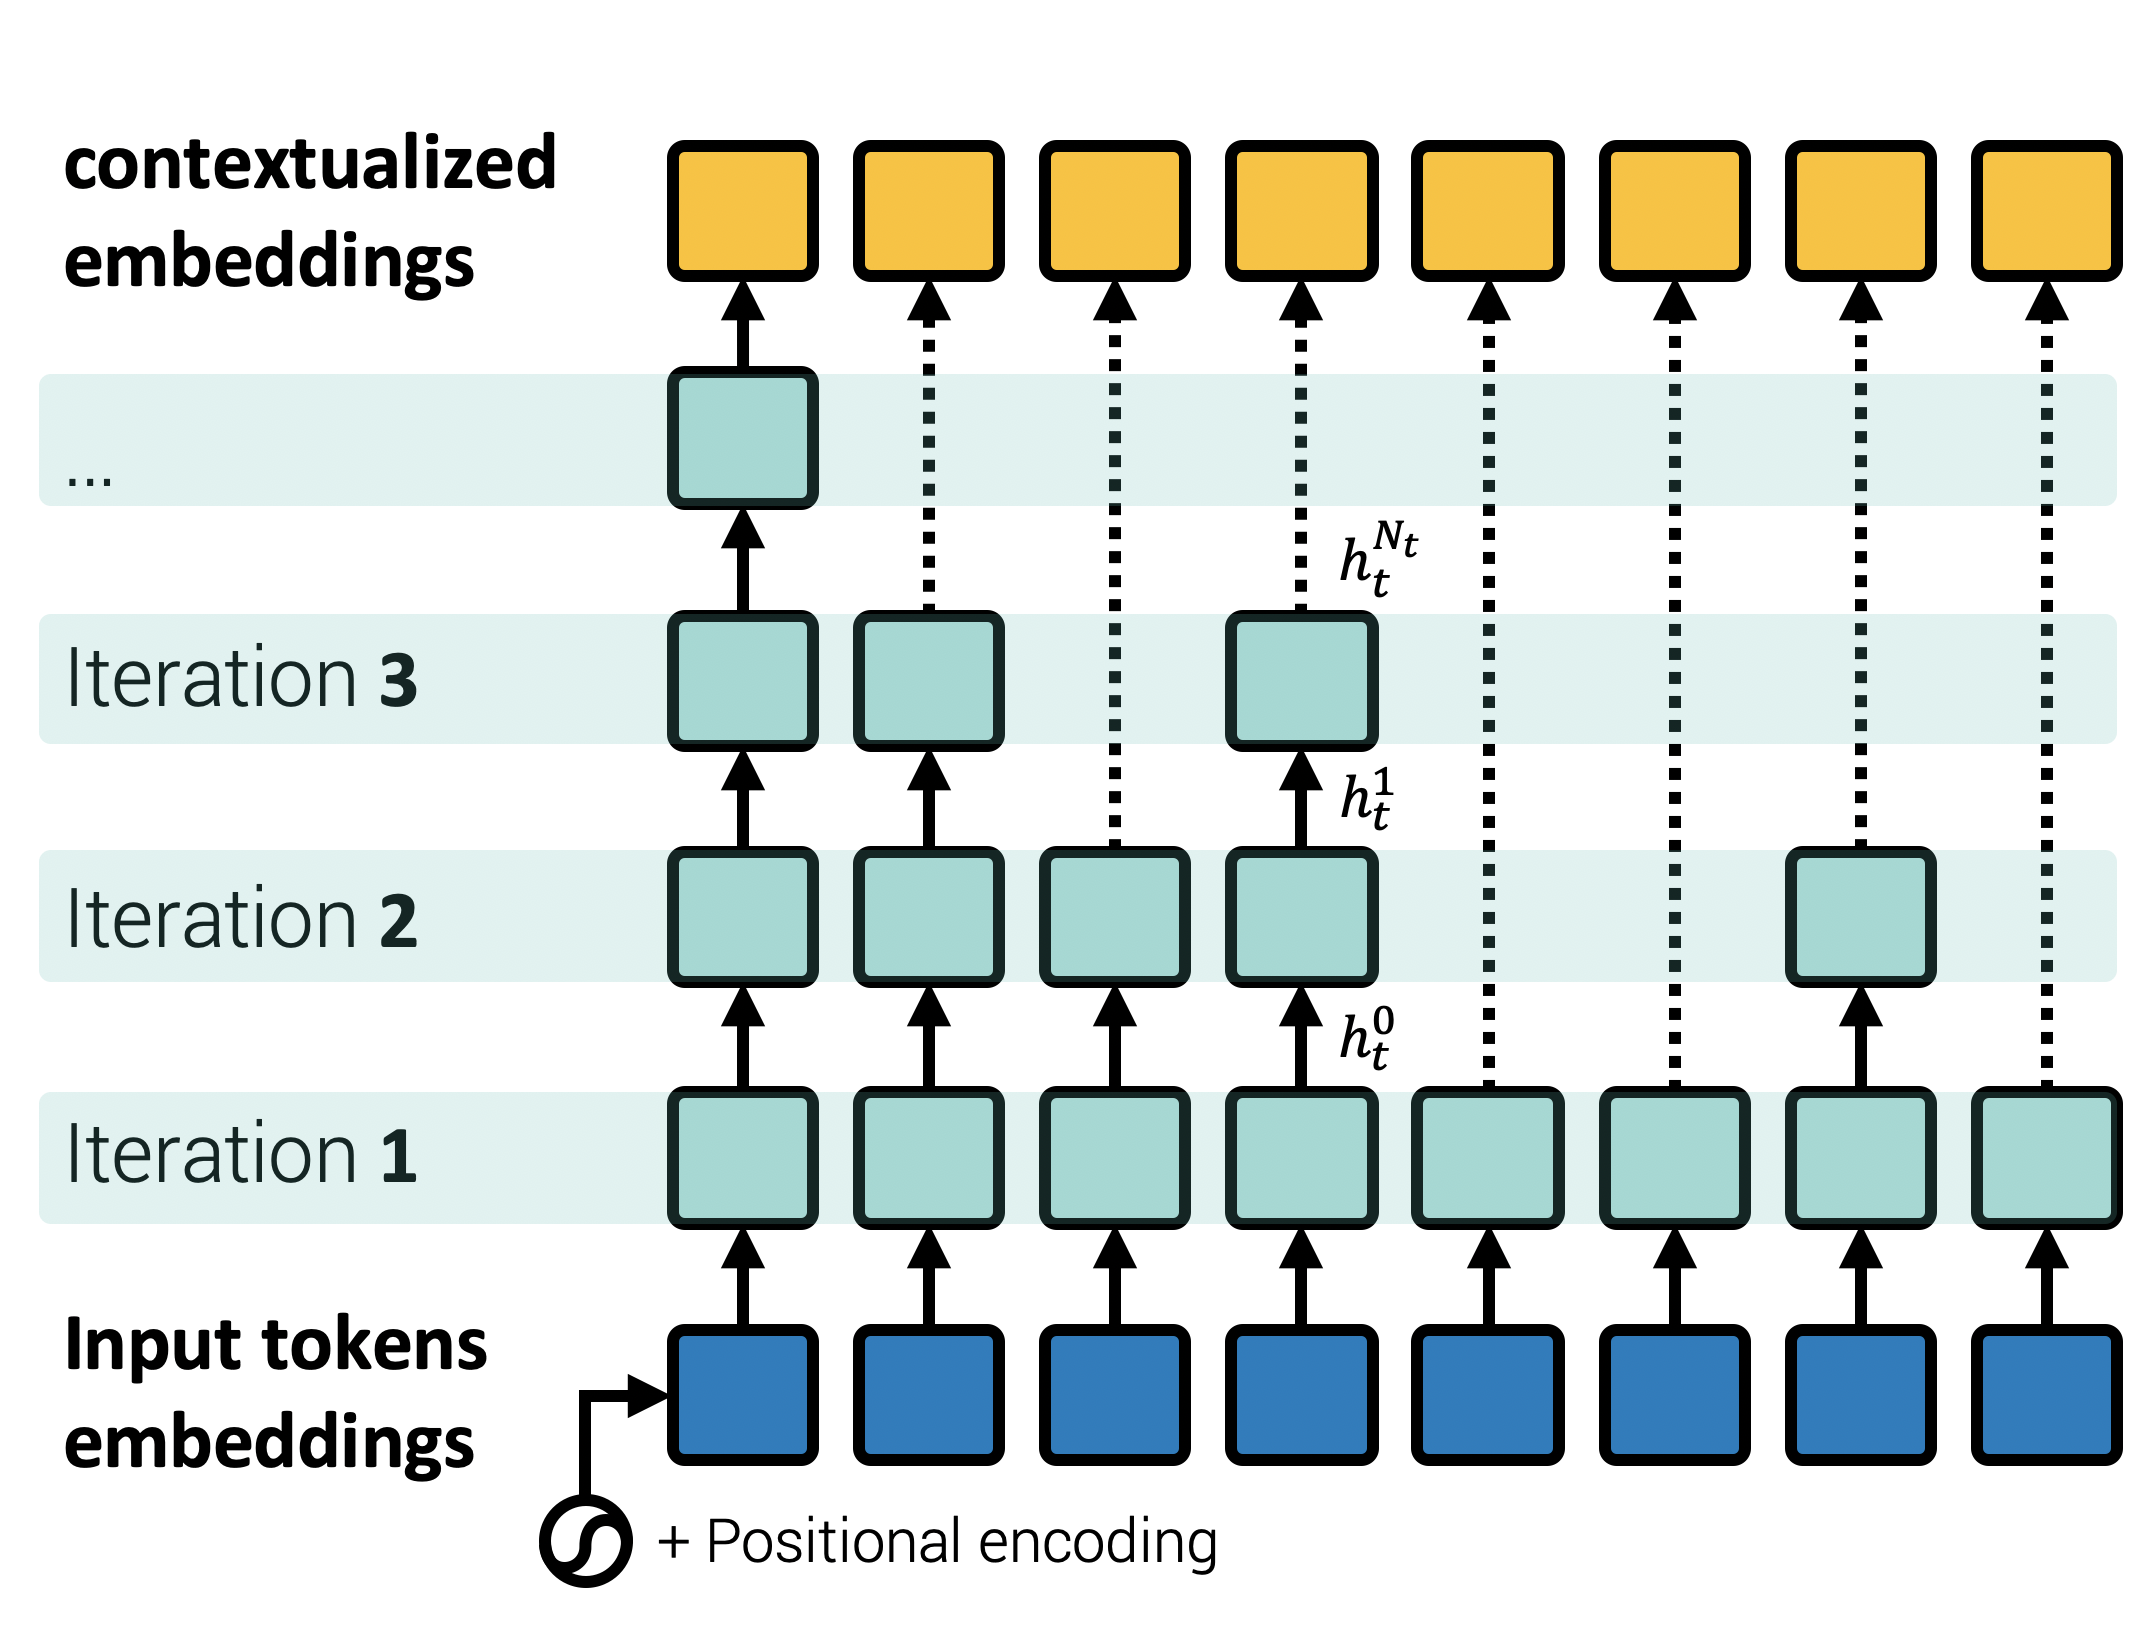
\includegraphics[width=8cm]{images/model-3.png}
\end{center}
\caption{As in \textsc{Albert}  model, tokens are transformed through the iterative application of a transformer encoder layer. Our model key specificity is the application of the halting mechanism, which dynamically adjusts the number of iterations for each token.
}
\labfig{transformers:model}
\end{figure}

\subsection{Pre-training objective}
\labsec{transformers:pre-training}

During the pre-training phase, we train the model with the sentence order prediction (\textit{sop}) — the task introduced in \textcite{lan_20} that classifies whether segments from the input sequence follow the original order or were swapped — and the masked language model task (\textit{mlm}) \parencite{devlin_19}. We also encourage the network to minimize the number of iterations by directly adding the ponder cost into \textsc{Albert}  pre-training objective. Given a length $T$ input sequence $\textbf{u}$,  \textcite{graves_16} defines the \emph{ponder cost} $\mathcal{P}(\textbf{u})$ as:
\begin{equation}
% \mathcal{P}(\textbf{u}) &= \sum_{t=1}^T N_{t} + R_t^{N_{t}-1} \label{eq:ponder-cost}\\
\mathcal{P}(\textbf{u}) = \sum_{t=1}^T N_{t} + R_t \label{eq:ponder-cost}
\end{equation}

We define the final pre-training loss as the following sum:

\begin{equation}
\hat{\mathcal{L}} = \mathcal{L}_{sop} + \mathcal{L}_{mlm} + \tau \mathcal{P} \label{eq:ponder-loss}
\end{equation}
where $\tau$ is a \emph{time penalty} parameter that weights the relative cost of computation versus error.

\subsection{Datum and infrastructure} We follow the protocol from \textsc{Albert} and pre-train the model with \textsc{BookCorpus}~\parencite{zhu_15} and English Wikipedia. We reduce the maximum input length to 128 and the number of training steps to 112,500\sidenote{As emphasized in \url{https://github.com/google-research/bert}, longer sequences are computationally expensive. To lighten the pre-training process, they advise using 128 sentence length and increase the length to 512 only for the last 10\% of the training to train the positional embeddings. In this work, we only perform the first 90\% steps as we are not looking for brute force performances.}. We use a lowercase vocabulary of size 30,000 tokenized using SentencePiece. We train all our models on a single TPU v2-8 from Google Colab Pro\sidenote{\url{https://colab.research.google.com/}} and accumulate gradients to preserve a 4,096 batch size. We optimize the parameters using \textsc{Lamb} with a learning rate at 1.76e-3.

\section{Experiments}
\labsec{transformers:experiments}

%We presented in Section~\ref{sec:method} the architecture of our iterative transformer model. 
We now analyze our iterative model properties during pre-training (\refsec{transformers:analysis-pretraining}) and fine-tuning (\refsec{transformers:analysis-downstream}). We start by describing the setup for each of the subtasks.

% \subsection{Experimental setup}
% \label{sub-sec:experimental-setup}

\paragraph{\textit{mlm} task} We generate masked inputs following \textsc{Albert} $n$-gram masking. We mask 20\% of all WordPiece tokens but do not always replace masked words with the \texttt{[MASK]} token to avoid discrepancy between pre-training and fine-tuning. We effectively replace 80\% of the masked position with \texttt{[MASK]} (\texttt{[MASK/MASK]}), 10\% with a random token (\texttt{[MASK/random]}), and keep the original token for the last 10\% (\texttt{[MASK/original]}).

\paragraph{\textit{sop} task} \bcomment{expand sop what does it mean?}{} We format our inputs as ``\texttt{[CLS]} $x_1$ \texttt{[SEP]} $x_2$ \texttt{[SEP]}''. In 50\% of the case the two segments $x_1$ and $x_2$ are effectively consecutive in the text. In the other 50\%, the segments are swapped. 
% The \textit{sop} task discriminates between the two cases.

\paragraph{Ponder cost} We fix the time penalty factor $\tau$ empirically such that the ponder penalty represents around 10\% of the total loss. To estimate the ponder cost, we discard the remainder, as $R \ll N$ for sufficient values of $N$. Given Eq.~\ref{eq:ponder-cost}, the ponder cost then corresponds to the total number of iterations in the sentence, which is given by $l \times T$, with $T$ the number of tokens in the sequence and $l$ the average iterations per token. We observe that \textsc{Albert} base loss converges to around 3.5. We calibrate $\tau$ such that  $\tau\mathcal{P} \approx 0.35 \approx \tau \times l \times T$. We train distinct models, listed in \reftab{transformers:pre-training}, that we calibrate such that their average number of iterations per token $l$ is respectively 3, 6, and 12. We refer to these models as respectively \textit{tiny}, \textit{small} and \textit{base}. 

\subsection{Analysis of the pre-training}
\labsec{transformers:analysis-pretraining}

% \begin{table*}[!htb]
% \small
% \renewcommand{\arraystretch}{1.2}
% \begin{center}
%  \begin{tabular*}{\textwidth}{l@{\extracolsep{\fill}}cccccccc c}
%     \toprule
%  &  MNLI-(m/mm)    & QQP        & QNLI       & SST-2      & CoLA       & STS-B      & MRPC       & RTE        & \textbf{Average} \\
%  & 392k            & 363k       & 108k       & 67k        & 8.5k       & 5.7k       & 3.5k       & 2.5k       & -          \\ 
% % \midrule\multicolumn{10}{c}{\it GLUE Leaderboard} \\\midrule
% % Pre-OpenAI SOTA    & 80.6/80.1       & 66.1       & 82.3       & 93.2       & 35.0       & 81.0       & 86.0       & 61.7       & 74.0       \\
% % BiLSTM+ELMo+Attn   & 76.4/76.1       & 64.8       & 79.8       & 90.4       & 36.0       & 73.3       & 84.9       & 56.8       & 71.0       \\
% % OpenAI GPT         & 82.1/81.4       & 70.3       & 87.4       & 91.3       & 45.4       & 80.0       & 82.3       & 56.0       & 75.1       \\
% % \textsc{Bert}-base          & 84.6/83.4       & 71.2       & 90.5       & 93.5       & 52.1       & 85.8       & 88.9       & 66.4       & 79.6       \\
% % \textsc{Albert}-base          & 84.6/83.4       & 71.2       & 90.5       & 93.5       & 52.1       & 85.8       & 88.9       & 66.4       & 79.6       \\
% \midrule\multicolumn{10}{c}{\it GLUE Leaderboard Reproductions} \\\midrule
% \textsc{Bert}-base          & 82.3/81.4       & 70.8       & 89.3       & 92.0       & 38.8       & 84.0       & 87.1       & 65.4       & 76.9       \\
% \textsc{Albert}-base          & ---/---       & ---       & ---       & ---       & ---       & ---       & ---       & ---       & ---       \\
% \midrule\multicolumn{10}{c}{\it Our Models} \\\midrule
% \textsc{Albert}-tiny + Adapt. Depth          & 77.0/76.8   & 67.8    & 86.4       & 87.6       & 27.5       & 81.8         &  84.7       & 62.0       & 72.6       \\
% \textsc{Albert}-small + Adapt. Depth          &   79.5/78.5     & 67.8       & 88.3       & 88.6       & 33.8       & 82.7       & 85.2      & 61.9       & 74.2       \\
% \textsc{Albert}-base + Adapt. Depth          & 79.9/79.2       & 68.5       & 89.0       & 87.8       & 36.7       & 84.2       & 86.5       & 63.0       & 75.2       \\
%     \bottomrule
%    \end{tabular*}
%    \caption{GLUE Test results}
%    \label{tab:glue_official}
% \end{center}
% \end{table*}

\paragraph{Analysis of the iterations} We pre-train models with various configurations and observe the model mechanisms during the pre-training in \reftab{transformers:pre-training}. 

\begin{table}[!htb]
% \footnotesize
\small
% \begin{minipage}{\textwidth}
\centering {
\begin{tabularx}{\textwidth}{l@{\extracolsep{\fill}}c c c c@{}}
\toprule
Models & \textit{tiny} & \textit{small} & \textit{base}\\
\midrule
% $\tau$ & 1e-3 & 5e-4 & 2.5e-4\\
% Max iterations & 6 & 12 & 24\\
% mlm (Acc.) & 55.4 & 57.1 & 57.4\\
% sop (Acc.) & 80.9 & 83.9 & 84.3\\
% \midrule
% All tokens & 3.8 & 6.9 & 9.8\\
% % \textbf{[MASK]} & 5.8 & 10.9 & 16\\
% All unmasked tokens & 3.6 & 6.4 & 9.2\\\relax
% \texttt[MASK/MASK]} & 5.8 & 10.9 & 16.0\\\relax
% \texttt[MASK/random]} & 5.8 & 10.9 & 16.0\\\relax
% \texttt[MASK/original]} & 4.0 & 7.4 & 10.5\\\relax
% \texttt[CLS]} & 5.7 & 10.4 & 18.9\\\relax
% \texttt[SEP]} & 2.3 & 5.7 & 8.1\\
$\tau$ & 1e-3 & 5e-4 & 2.5e-4\\
Max iterations & 6 & 12 & 24\\
mlm (Acc.) & 55.4 & 57.1 & 57.4\\
sop (Acc.) & 80.9 & 83.9 & 84.3\\
\midrule
All tokens & 3.8 & 7.1 & 10.0\\
All unmasked tokens & 3.5 & 6.5 & 9.2\\\relax
\texttt{[MASK/MASK]} & 5.8 & 10.9 & 16.0\\\relax
\texttt{[MASK/random]} & 5.8 & 10.9 & 16.0\\\relax
\texttt{[MASK/original]} & 4.0 & 7.4 & 10.5\\\relax
\texttt{[CLS]} & 6.0 & 12.0 & 22.5\\\relax
\texttt{[SEP]} & 2.5 & 7.6 & 8.4\\
\bottomrule
\end{tabularx}}
\caption{Average number of iterations given token types during the pre-training. For each model, we report a mean number of iterations on our development set, at the end of the pre-training. 
%We make the distinction between each configuration.
}
\labtab{transformers:pre-training}
\end{table}

% Regarding the special tokens, we confirm results advanced by the analysis of \textsc{Bert}  attention patterns \parencite{clark_19}. 
We observe that the \texttt{[CLS]} token receives far more iterations than other tokens. This observation is in line with \textcite{clark_19} who analyze \textsc{Bert}  attention and report systematic and broad attention to special tokens. We interpret that the \texttt{[CLS]} token is used as input for the \textit{sop} task and aggregates a representation for the entire input. On the contrary, \texttt{[SEP]} token benefits from usually few iterations. Again, this backs \bcomment{up}{} the observation emerging from the analysis of attention that interprets \texttt{[SEP]} as a no-op operation for attention heads \parencite{clark_19}.

% We interpret that the \texttt{[CLS]} token is used for the \textit{sop} objective, which depends on every other token in the sentence. The \texttt{[CLS]} token acts as an artificial root of the sentence and needs other tokens to converge before its.   

We also observe an interesting behavior from the \texttt{[MASK]} which also benefits from more iterations than average tokens. As for the \texttt{[CLS]} token, we interpret that these tokens are crucial for the \textit{mlm} task. Looking further, we observe that \texttt{[MASK/random]} and \texttt{[MASK/MASK]} number of iterations is greater than \texttt{[MASK/original]}. In this case, although all tokens are targeted in the \textit{mlm} task, \texttt{[MASK/random]} and \texttt{[MASK/MASK]} are  obviously more difficult to identify\sidenote{During inference, the model cannot make the distinction between \texttt{[MASK/original]} and unmasked tokens. However, we observe in \reftab{transformers:pre-training} that the two token types have a distinct mean number of iterations. We believe this is due to the distribution of the \texttt{[MASK]} tokens. Indeed, we follow the procedure from \textsc{Albert}  and use \textit{n-gram} masking. Therefore, \texttt{[MASK/original]} tokens tend to appear in the context of \texttt{[MASK]} tokens. This specific context increases the mean number of iterations.}.
%more explicit and less difficult to identify than

The model seems to have an intuitive mechanism and distributes iterations for tokens that are either crucial for the pre-training task or present a certain level of difficulty. This also appears in line with \textit{early-exit} mechanisms cited in \refsec{transformers:dynamic-depth}, that adapt the number of layers, for the whole example, to better scale to each sample level of difficulty.

% We observe that mask tokens benefit from more iterations. We observe a discrepancy between these categories. In particular, when the mask token is unchanged, the number of iterations stands between unmask tokens and other mask tokens. We interpret that tokens are directly driven by the loss benefit from more iterations and that, as expected, ambiguous tokens such as \texttt{[MASK]} require more iterations.

\paragraph{Natural Fixed point} We now analyze \textit{how} the token's hidden states evolve during our model iterative transformations. At each iteration $n$, the self-attentive mechanism \parencite{vaswani_17} computes the updated state $n+1$ as a weighted sum of the current states. This introduces a cyclic dependency as every token depends on each other during the iterative process. As convergence within a loopy structure is not guaranteed, we encourage the model to converge towards a fixed point \parencite{bai_19}.

\begin{figure}[!htb]
\begin{center}
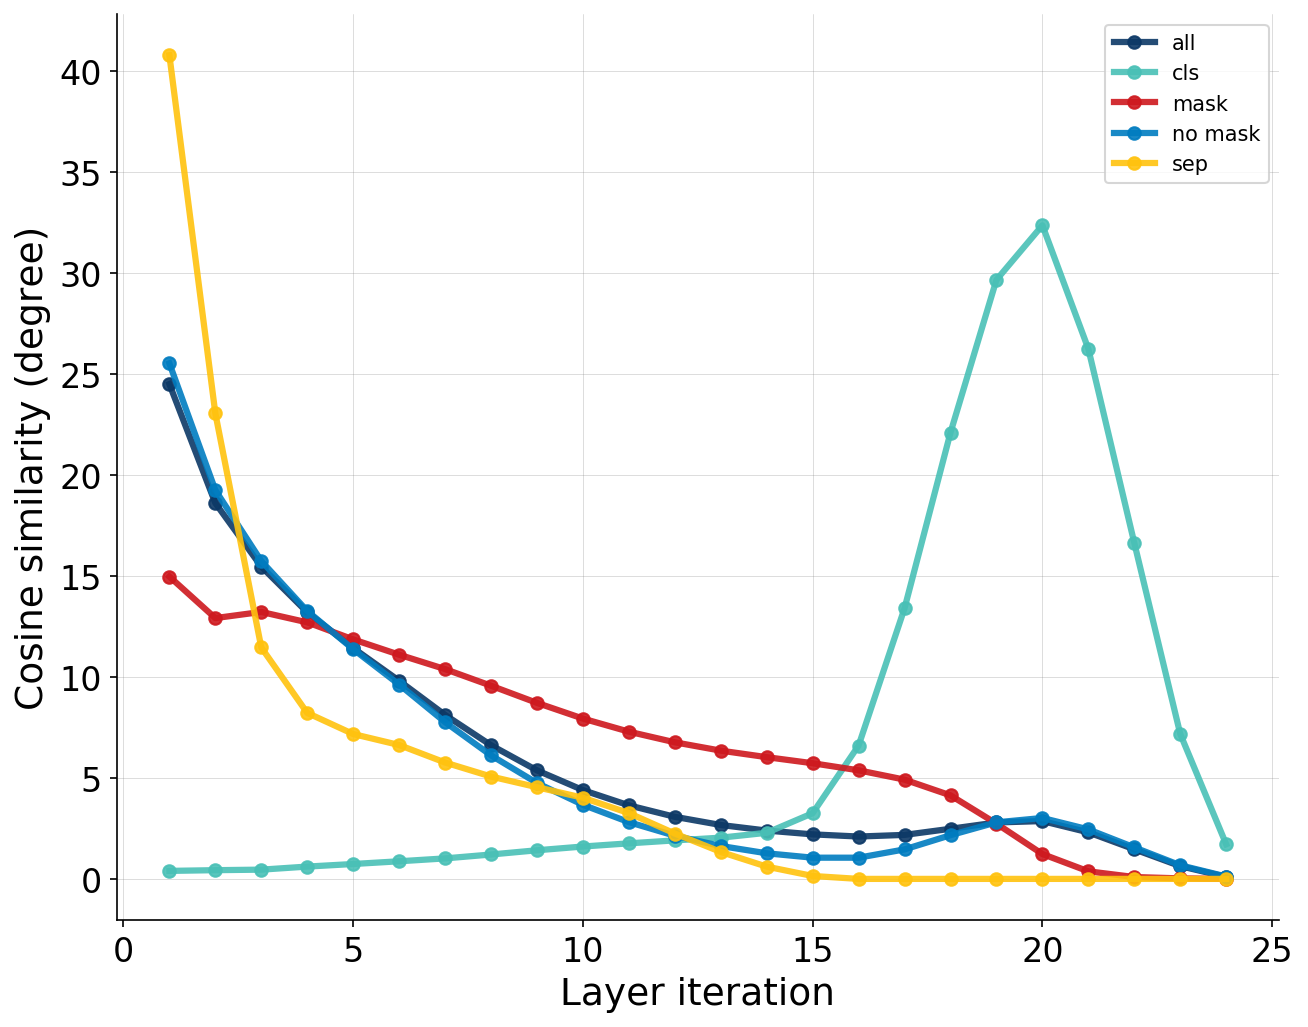
\includegraphics[width=8cm]{images/cosine-base-v3 (1).png}
\end{center}
\caption{Evolution of the cosine similarity between hidden states $h^n_t$ and $h^{n+1}_t$ from two consecutive iterations. We use our \textit{base} model and measure iterations on our development set, at the end of the pre-training.}
\labfig{fixed-point}
\end{figure}

We obtain this property "for free" thanks to our architecture specificity. Indeed at each iteration, the hidden state is computed as a convex combination of the previous $n$ and current $n+1$ hidden state. The combination is controlled by $\lambda^n_t$  (Eq.~\ref{eq:halting-3}). If $\lambda^n_t$ is closed to $0$, then $h^n_t \approx h^{n+1}_t$ and by definition (Eq.~\ref{eq:halting-22}, \ref{eq:halting-r}) $\lambda^n_t$ will eventually be set to $0$ at a certain iteration.

% we encourage the model to reach a fixed point \parencite{bai_19}. Indeed, transformers induce a dependency between every token in the sentence as the self-attentive mechanism \parencite{vaswani_17} computes each state as a weighted sum from each other. This introduces a cyclic dependency between each token. Convergence within a loopy structure is known to be uncertain. We encourage the model to reach a fixed point, to facilitate the convergence process. 

% By design, we encourage the model to converge toward a fixed point. This property may be used as a sole training objective \parencite{bai_19} while we obtain this property "for free" thanks to the specificity of our architecture. 


\reffig{fixed-point} represents the evolution of the mean cosine similarity between two hidden states from two consecutive iterations $h^n_t$ and $h^{n+1}_t$. The network indeed reaches a fixed point for every token. The \texttt{[SEP]} and tokens that are not masked converge quicker than \texttt{[MASK]} tokens. Finally, the \texttt{[CLS]} token oscillates during intermediate layers before reaching an equilibrium.
% \sidenote{We present the Figures for other model configurations in Appendix~\ref{appendix:natural-fixed-point}}.

\subsection{Application to downstream tasks}
\labsec{transformers:analysis-downstream}

During the pre-training phase, the model focuses on tokens  either crucial for the pre-training task or \bcomment{that}{} present a certain level of difficulty. Now we study our model behavior during the fine-tuning on downstream syntactic or semantic tasks.


\paragraph{Control test} To verify that our setup has reasonable performance, we evaluate it on the GLUE benchmark \parencite{wang_19}.
% \sidenote{We provide experimental details in Appendix~\ref{appendix:glue}}. 
Results from \reftab{glue-official} are scored by the evaluation server\sidenote{\url{https://gluebenchmark.com/leaderboard}}. As in \textcite{devlin_19}, we discard results for the WNLI task\sidenote{See point (12) from \url{https://gluebenchmark.com/faq}.}. For each task, we fine-tune the model on the train set and select the hyperparameters on the dev set using a grid search. We tune the learning rate between 5e-5, 3e-5, and 2e-5; batch size between 16 and 32 and epochs between 2, 3, or 4. To better compare our setup, we pre-train \textsc{Bert} and \textsc{Albert} model using our configuration, infrastructure and datum.

\begin{table}[!htb]
\small
%\renewcommand{\arraystretch}{1.2}
\centering {
\begin{tabularx}{\textwidth}{l@{\extracolsep{\fill}} Y Y@{}}
\toprule
& \textbf{Avg. Glue score} \\
\midrule
\textsc{Bert}-base   & 76.9       \\
\textsc{Albert}-base   & 75.6       \\
\midrule
\textsc{Albert}-base + Adapt. Depth  & 75.2       \\
\textsc{Albert}-small + Adapt. Depth     & 74.2       \\
\textsc{Albert}-tiny + Adapt. Depth       & 72.6       \\
\bottomrule
\end{tabularx}}
\caption{GLUE Test results, scored by the evaluation server but without the WNLI task. To facilitate the comparison, we reproduce \textsc{Bert} and \textsc{Albert}, with our pre-training dataset, infrastructure and configuration detailed in \refsec{transformers:pre-training}.}
\labtab{glue-official}
\end{table}


We present results on the test set in \reftab{glue-official}. As expected, the average score decreases with the number of iterations. Indeed, we limit the number of computation operations performed by our model. Moreover, we build our model on top of \textsc{Albert} , which share parameters across layers, thus reducing the number of parameters compared with the original \textsc{Bert}  architecture. However, despite these additional constraints, results stay in a reasonable range. In particular, \textsc{Albert}-base with adaptative depth is very close to the version with a fixed depth. 
%Although, as detailed in Table~\ref{table:pre-training}, tokens perform in average only 10 iterations compared to 12 for \textsc{Albert}-base.

%\sidenotetext{See (10) in \url{https://gluebenchmark.com/faq}.}
% . scored by the evaluation server ({\small \url{https://gluebenchmark.com/leaderboard}}). The number below each task denotes the number of training examples. The ``Average'' column is slightly different than the official GLUE score. since we exclude the problematic WNLI set.\sidenote{See question 10 in \url{https://gluebenchmark.com/faq}.} 
   %OpenAI GPT = (L=12. H=768. A=12); \textsc{Bert} base = (L=12. H=768. A=12); \textsc{Bert} large = (L=24. H=1024. A=16).  BERT and OpenAI GPT are single-model. single task. F1 scores are reported for QQP and MRPC. Spearman correlations are reported for STS-B. and accuracy scores are reported for the other tasks. We exclude entries that use BERT as one of their components.

\paragraph{Probing tasks} \textcite{conneau_18} introduce probing tasks, which assess whether a model encodes elementary linguistic properties. We consider semantic and syntactic tasks that do not introduce random replacements. In particular, a task that predicts the sequence of top constituents immediately below the sentence node (TopConst) \bcomment{prvode an example}{}, a task that predicts the tense of the main-clause verb (Tense) \bcomment{prvode an example}{}, and two tasks that predict the subject (resp. direct object) number in the main clause (SubjNum, resp. ObjNum). \bcomment{prvode an example}{}

% model base warm up 200 5e-5
\begin{table}[!htb]
\small
% \begin{minipage}{\textwidth}
\centering {
\begin{tabularx}{\textwidth}{l@{\extracolsep{\fill}}Y Y Y Y Y@{}}
\toprule
  & Tense & Subj Num & Obj Num & Top Const\\
\midrule
punct (121k)      & 5.0 & 4.8 & 5.2 & 6.7\\
prep (101k)      & 4.6 & 4.6 & 5.4 & 6.2\\
pobj (98k)      & 4.5 & 4.6 & 5.4 & 5.8\\
det (86k)      & 4.5 & 4.6 & 5.1 & 6.1\\
nn (81k)     & 5.1 & 5.4 & \textbf{5.8} & 6.7\\
nsubj (80k)      & \textbf{5.3} & \textbf{6.1} & \textbf{5.9} & \textbf{7.5}\\
amod (66k)     & 4.6 & 4.9 & 5.5 & 6.1 \\
dobj (49k)     & 4.8 & 5.0 & \textbf{5.9} & 6.1 \\
root (44k)     & \textbf{5.9} & \textbf{6.1} & \textbf{6.2} & \textbf{7.9} \\
advmod (37k)     & 4.8 & 4.8 & 5.3 & 6.8 \\
\midrule
avg.      & 5.4 & 5.4 & 5.8 & 7.2 \\
% std.      & 0.2 & 0.3 & 0.2 & 0.5 \\
test Acc.      & 87.5 & 93.9 & 96.1 & 91.2 \\
baseline Acc.      & 87.3 & 94.0 & 96.0 & 91.9 \\
\bottomrule
\end{tabularx}}
\caption{Distribution of the iterations across token dependency types. We fine-tune our \textit{base} model on each probing task. We then perform inference on the Penn Tree Bank dataset and report the number of iterations given token dependency types. The number in parentheses denotes \bcomment{the number of dependency tags}. We only display the top 10 most frequent tags. We indicate in \textbf{bold} tags  for  which the number of iterations is above avg + std. We include a baseline accuracy which we obtain with the \textsc{Albert}-base version without an adaptative depth mechanism and therefore 12 iterations performed for each token.}
\labtab{table:probing}
\end{table}

% model small warm up 3000 5e-5
% \begin{table}[!htb]
% \small
% % \begin{minipage}{\textwidth}
% \centering {
% \begin{tabularx}{\textwidth}{l@{\extracolsep{\fill}}Y Y Y Y Y@{}}
% \toprule
%   & Tense & Subj Num & Obj Num & Top Const\\
% \midrule
% punct (121k)      & 3.2 & 2.6 & 3.4 & 3.8\\
% prep (101k)      & 3.0 & 2.5 & 3.1 & 3.3\\
% pobj (98k)      & 3.0 & 2.6 & 3.1 & 3.2\\
% det (86k)      & 2.9 & 2.4 & 3.0 & 3.4\\
% nn (81k)     & 3.2 & \textbf{3.0} & 3.3 & 3.6\\
% nsubj (80k)      & \textbf{3.4} & \textbf{3.2} & \textbf{3.3} & \textbf{4.1}\\
% amod (66k)     & 3.0 & 2.6 & 3.2 & 3.4 \\
% dobj (49k)     & 3.1 & 2.7 & \textbf{3.5} & 3.4 \\
% root (44k)     & \textbf{3.6} & \textbf{3.1} & \textbf{3.7} & \textbf{4.4} \\
% advmod (37k)     & 3.1 & 2.5 & 3.2 & 3.7 \\
% \midrule
% avg.      & 3.2 & 2.8 & 3.4 & 3.6 \\
% % std.      & 0.2 & 0.3 & 0.2 & 0.5 \\
% test Acc.      & 89.8 & 93.0 & 94.7 & 90.8 \\
% baseline Acc.      & 90.6 & 93.3 & 96.1 & 91.3 \\

% \bottomrule
% \end{tabularx}}
% \caption{Distribution of the iteration across token dependency types. We fine-tune our \textit{small} model on each probing task. We the perform inference on the Penn Tree Bank dataset and report the number of iterations given token dependency types. The number in parentheses denotes the number of dependency tags. We only display the top 10 most frequent tags. We indicate in \textbf{bold} tags  for  which the iteration is above avg + std. We include a baseline accuracy which we obtain with the \textsc{Albert} -base version without an adaptative depth mechanism and therefore 12 iterations performed for each token.}
% \label{table:probing}
% \end{table}

% model base warm up 3000 5e-5
% \begin{table}[!htb]
% \small
% % \begin{minipage}{\textwidth}
% \centering {
% \begin{tabularx}{\textwidth}{l@{\extracolsep{\fill}}Y Y Y Y Y@{}}
% \toprule
%   & Tense & Subj Num & Obj Num & Top Const\\
% \midrule
% punct (121k)      & 7.2 & 6.6 & 7.1 & \textbf{7.0}\\
% prep (101k)      & 6.6 & 6.0 & 6.9 & 6.1\\
% pobj (98k)      & 6.7 & 6.0 & 7.0 & 5.9\\
% det (86k)      & 6.5 & 5.9 & 6.6 & 6.2\\
% nn (81k)     & 7.2 & 6.8 & 7.4 & 6.5\\
% nsubj (80k)      & \textbf{7.6} & \textbf{7.5} & \textbf{7.6} & \textbf{7.6}\\
% amod (66k)     & 6.6 & 6.1 & 6.9 & 6.0 \\
% dobj (49k)     & 6.9 & 6.3 & \textbf{7.5} & 6.0 \\
% root (44k)     & \textbf{8.1} & \textbf{7.7} & \textbf{7.9} & \textbf{7.7} \\
% advmod (37k)     & 6.8 & 6.3 & 6.9 & \textbf{6.9} \\
% \midrule
% avg.      & 7.5 & 6.9 & 7.7 & 7.2 \\
% % std.      & 0.2 & 0.3 & 0.2 & 0.5 \\
% test Acc.      & 90.4 & 94.2 & 95.9 & 91.1 \\
% baseline Acc.      & 90.6 & 93.3 & 96.1 & 91.3 \\

% \bottomrule
% \end{tabularx}}
% \caption{Distribution of the iteration across token dependency types. We fine-tune our \textit{small} model on each probing task. We the perform inference on the Penn Tree Bank dataset and report the number of iterations given token dependency types. The number in parentheses denotes the number of dependency tags. We only display the top 10 most frequent tags. We indicate in \textbf{bold} tags  for  which the iteration is above avg + std. We include a baseline accuracy which we obtain with the \textsc{Albert} -base version without an adaptative depth mechanism and therefore 12 iterations performed for each token.}
% \label{table:probing}
% \end{table}

In our setup, we fine-tune the model on the task train set and select the hyperparameters on the dev set using a grid search. We use a 5e-5 learning rate and fine tune the epochs between 1 to 5; we use a 32 batch size.
%we fine-tune the model on the task train set. We select the best number of training steps on the dev set. 
Finally, we %perform inference and 
compare in Table~\reftab{table:probing} the number of iterations performed for each token 
% measure the number of iterations performed for each token 
on the Penn Tree Bank \parencite{marcus_94} converted to Stanford dependencies\sidenote{Since we use sentence piece vocabulary, we assign to each piece the dependency tag from the whole token.}.
%\sidenote{We present the Tables for other model configurations in Appendix~\ref{appendix:probing}}.
% We compare in Table~\ref{table:probing} the number of iterations performed for each token 

We provide an accuracy baseline, obtained with the same setup but using \textsc{Albert}  without the dynamic halting mechanism. As in the previous experiment, we observe that for these tasks, our model achieve competitive performances despite using less computational operations.

Although all tasks achieve significant and comparable accuracies, they all require a distinct global mean of iterations. The Tense task, which can be solved from the verb only, is completed in only 5.4 iterations, while the TopConst task, which requires to infer some sentence structure, is performed in \bcomment{7.2} iterations. This suggests the model can adapt itself to the complexity of the task and globally spare unnecessary iterations. 

Looking at the token level, as during the pre-training (\refsec{transformers:analysis-pretraining}), the iterations are unevenly distributed across tokens. The model seems to iterate more on tokens that are crucial for the task. For SubjNum, the subj tokens achieve the maximum number of iterations, while for the ObjNum task, the obj and root token iterates more. Similarly, all tasks present a high number of iteration on the main verb (root) that is crucial for each prediction.

\section{Conclusion}
% We propose a transformer pre-trained model that adapts the number of layer iterations performed on each token. We assume that language have a recursive structure where tokens, such as verbs, induce more dependence with other tokens than determinant or adverbs for example. We hypothesize that computing contextualized representation for a given token requires first computing the representation for its dependants. Therefore, we expect low dependency tokens to quickly converge in the early layer, while highly dependent, complex, or ambiguous tokens would converge in later layers. Exiting the process early for low dependency or explicit tokens may spare some computations and avoid interference with the global convergence process.

% To this end, 
We investigated the role of the layers in deep transformers. We designed an original model that progressively transforms each token through a dynamic number of iterations. We analyzed the distribution of these iterations during pre-training and confirmed the results obtained by analyzing the distribution of attention across \textsc{Bert}  layers, particularly the specific behavior played by special tokens. Moreover, we observed that key tokens for the prediction task benefit from more iterations. We confirmed this observation during fine-tuning, where the tokens with a large number of iterations are also suspected to be key for achieving the task.

Our experiments provide a new interpretation path for the role of layers in deep transformer models. Rather than extracting some specific features at each stage, layers could be interpreted as the iteration from an iterative and \bcomment{convergence}{convergent} process. We hope that this can help to better understand the convergence mechanisms for transformers models, reduce the computational footprint or provide new regularization methods.

% \setchapterimage[7.5cm]{seaside}
\setchapterstyle{kao}
\setchapterpreamble[u]{\margintoc}
%\chapter[Figures and Tables]{Figures and Tables\footnotemark[0]}
\chapter{Characterizing compositional properties of neural architectures}

\cleanchapterquote{
Cette langue serait merveilleuse \textup{[\,\dots]} car alors raisonner et calculer sera la même chose.}{Gottfried Wilhelm Leibniz
}{}


While transformers show outstanding performances on many NLP benchmarks, they also have some linguistic limitations. In particular, regarding their ability to generalize outside their training range and to learn elementary composition rules. The benchmark COGS \parencite{kim_2020} for example highlights deep learning models struggle to generalize to longer sequences or sentences with deeper level of recursion than seen during training. Following my work on integrating structure into neural architecture, I aim at better characterizing how the model structure may affect their degree of compositionality. This work is currently in an experimentation phase. I am building an evaluation setup with arithmetic expressions containing specific properties. I train various models on specific subsets and observe how models generalize outside their domain. In particular, I compare models relying on different degrees of structure constraints such as sequential, recursive, or unstructured models.


\section{Dataset description}

\section{Evaluation}

\section{Impact of the expression’s complexity}

\section{Enhancing model compositional abilities}




\pagelayout{wide} % No margins
\addpart{Training neural models at scale}
\pagelayout{margin} % Restore margins

\setchapterstyle{kao}
\setchapterpreamble[u]{\margintoc}
\chapter{Embedding sentences with large transformer models}
%Training sentence embedding models using discriminative objective}
\labch{1B}

\cleanchapterquote{Language is the most interesting manifestation of intelligence. Visual comprehension is something that many animals also have. In some cases, it is even better than that of humans. Chimpanzees also understand feelings and social contexts. But no other living being has such a complex language as we do. And language links all other manifestations of intelligence, because I can talk about what I see, feel and think and how I act.}{Richard Socher}{Interview for \textit{die Zeit}, 2019}
% Artificial Intelligence Doesn't Make After Work Plans
% https://www.zeit.de/digital/2019-05/computational-linguistics-artificial-intelligence-speech-processing-richard-socher?utm_referrer=https%3A%2F%2Ft.co%2F

% \bcomment{you might ask a more incisive question in the first place,suggesstion:}{\ldots }

Bigger is better ? at first sight it seems that current Natural Language Processing is consistently evolving towards larger and larger models paying less and less attention to the models at hand. In this section, we explore how we can leverage the performance of large sentence encoders by adapting their pre-training and increasing their size.

The previous sections discussed the importance of neural model structure in composing sentence representations. Yet, NLP trends do not primarily focus on these types of models, instead focusing on transformers, which are easier to scale. As a result, previous years have seen a general increase in the size of the models and a corresponding improvement over downstream performances. These improvements did not directly benefit sentence embeddings, as many transformer encoders perform below state-of-the-art on standard benchmarks. 
% In this section. we review the challenges and benefits of large models.

This section relates the development of state-of-the-art sentence embedding models as part of the project \textit{Train the Best Sentence Embedding Model Ever with 1B Training Pairs}.\footnote{\url{https://discuss.huggingface.co/t/train-the-best-sentence-embedding-model-ever-with-1b-training-pairs/7354}} This project took place during the \textit{Community week using JAX/Flax for NLP \& CV} organized by Hugging Face.\footnote{\url{https://discuss.huggingface.co/t/open-to-the-community-community-week-using-jax-flax-for-nlp-cv/7104}} Our project was among the competition winners and received an honorable mention. As part of this project, I contributed actively to the construction of the dataset as well as the training and documentation of the sentence embedding models.

We organize the section as follows: we first review the related work and the benefit of scaling in the specific case of sentence embeddings (\refsec{scale:introduction}). \refsec{scale:method} then proposes a self-supervised pre-training approach to learn sentence encoders. The approach addresses engineering challenges such as data collection, framework choice, or training hyper-parameters. Finally, we evaluate the benefit of our approach in \refsec{scale:experiments}.

\section{Transformers and scale}
\labsec{scale:introduction}

Pre-trained transformers resulted in a strong improvement over standard NLP benchmarks. The model \textsc{Bert} indeed claimed a 7.6\% absolute improvement on the popular GLUE benchmark, 5.6\% absolute accuracy improvement on the MultiNLI, and 1.5 F1 points on the SQuAD v1.1 question answering test. \textsc{Bert} introduced many increments to solve NLP tasks, including a new neural architecture, training paradigm number of parameters, and hyper-parameters setup. It is difficult to disentangle the contributions of all these factors, but the number of parameters is one of them. For example, the base version of \textsc{Bert} with 100M parameters achieves an average score of 79.6 on GLUE, while the large version with 340M parameters achieves 82.1. Apart from the number of parameters, the architecture, training procedure, and training data remain unchanged.

Compared with tree-structured encoders, transformers encode sentences without making substantial structure premises. Compared with sequential encoders, they compute each token state simultaneously using the attention mechanism, which is easy to parallelize across computing units. From a computing perspective, transformers are easier to scale. Consequently, the last few years have seen a race to increase the number of layers, parameters, hidden size, or pre-training data size. The model \textsc{Bert} exists in a base and large versions, which only differ by their hidden size and number of parameters. The same is true for the model GPT, which was incremented into GPT-2 and 3. While the second and third versions have much more parameters, the architecture is similar between all versions. As illustrated in \reffig{large-models}, the number of parameters for large language models follows what we may compare with Moore's Law.

% As opposed to deriving complex architectures from linguistic insights. it might be easier to focus on efficient and parallelizable networks. which are easy to scale. 

% Language models also seem to support the adage. "\bcomment{the bigger. the better}{bigger is better}".  The training at scale seems also to leverage some particular behaviors. mediated by some threshold effects. For example \textcite{brown_20} compare generative pre-trained models with distinct sizes on few-shot learning settings. While the smallest model with 1.3B parameters do not show any abilities on the task. the largest model with 175B parameters show surprisingly good generalization performances with a very limited number of training examples.

\begin{figure}[htb!]
	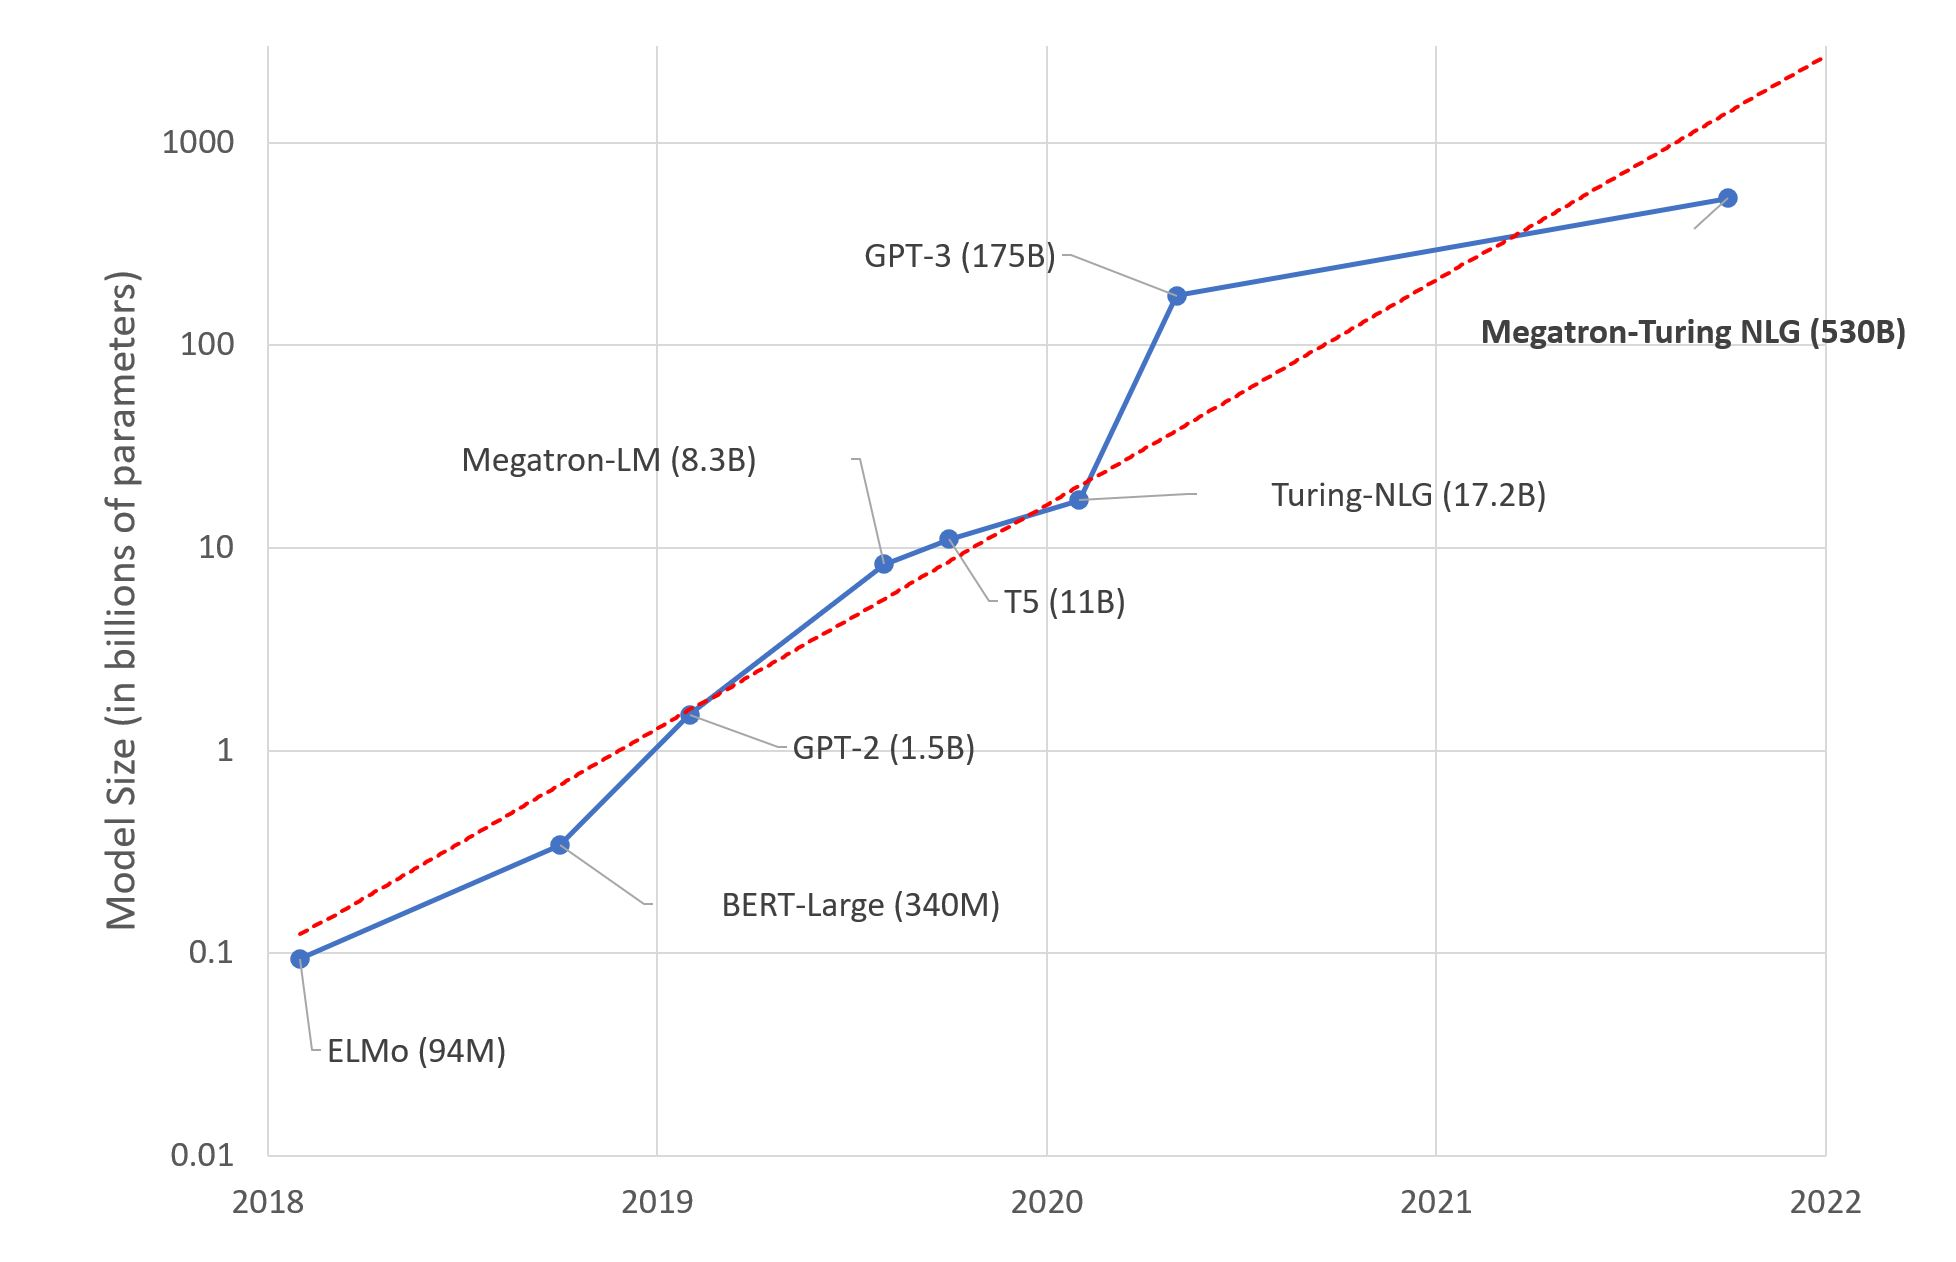
\includegraphics[width=\textwidth]{images/model-size-graph.jpeg}
	\caption[Large models number of parameters]{Evolution of the number of parameters for large language models. The figure is extracted from Microsoft \href{https://www.microsoft.com/en-us/research/blog/using-deepspeed-and-megatron-to-train-megatron-turing-nlg-530b-the-worlds-largest-and-most-powerful-generative-language-model/}{blog post}.}
	\labfig{large-models}
\end{figure}

This analysis also applies in some respects to sentence embeddings. As empirically observed by \textcite{conneau_17}, the embedding size is a key factor in downstream performances over the SentEval benchmark. We reproduce the figure from \textcite{conneau_17} in \reffig{scale:embedding-size}. For almost all encoders shown in the figure, performance increases proportionally to the size of the embeddings. However, regarding specifically \textsc{Bert}, the comparison does not directly extend to the embedding of sentences. Indeed, as already reported in \reftab{contrastive-soa}. \textsc{Bert} performance on the SentEval benchmark is, on average, 3 points below current state-of-the-art methods, including \textcite{simoulin_2021a}.

This lack of performance does not seem to be specifically related to the architecture of transformers. Indeed, \textcite{reimers_19} propose state-of-the-art sentence embeddings by successfully adapting the protocol from \textcite{conneau_17} to transformers. The approach successfully proposes to further fine-tune a pre-trained transformer on natural language inference data.

\begin{figure}[htb!]
	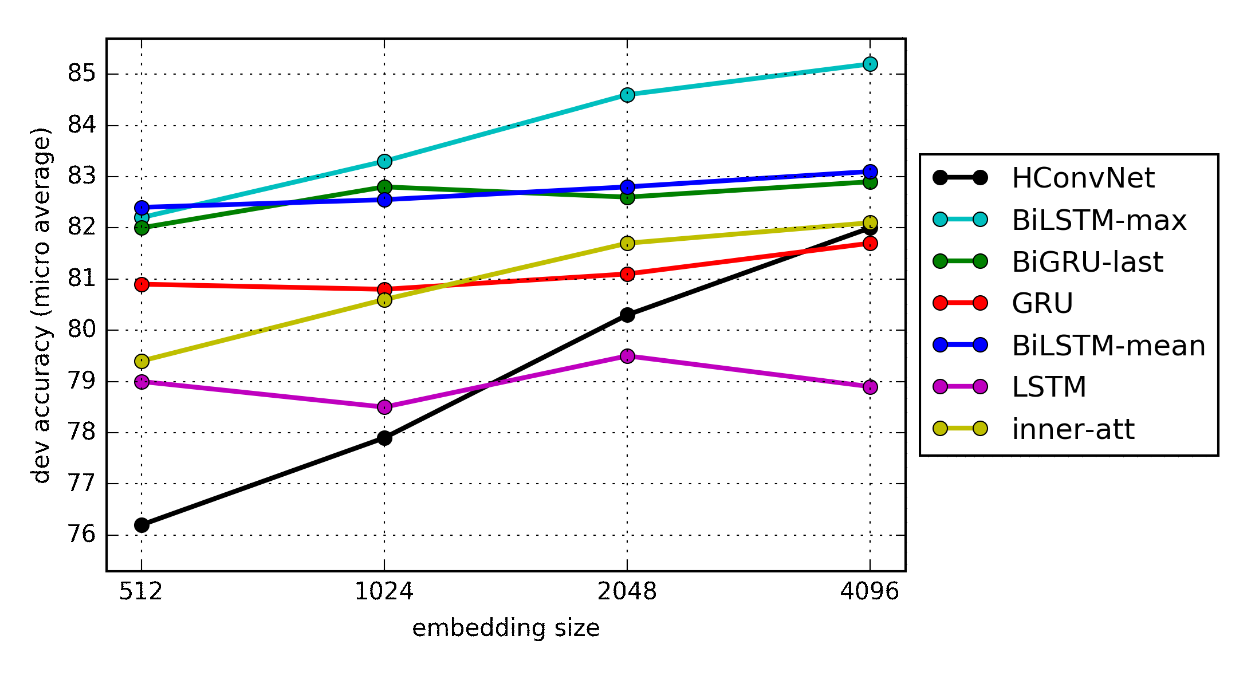
\includegraphics[width=\textwidth]{images/snli_em_size.png}
	\caption{Average performance with respect to the embedding size on the SentEval benchmark. The figure is extracted from \textcite{conneau_17}.}
	\labfig{scale:embedding-size}
\end{figure}

% Here. we study to which extend we can increase sentence encoder performances by scaling their size. As already observed in \refch{arithmetics} or \refsec{survey:downstream}. scaling models is an established method for improving downstream results. However. 

% \bcomment{The previous sections discussed the importance of neural model structure in composing sentence representations. Along with the architecture of the sentence encoder. other parameters may strongly influence the quality of the embeddings. In particular. the last few years have seen a race to increase the number of parameters. hidden size. or size of pre-training data. As already observed in \refch{arithmetics} or \refsec{survey:downstream}. scaling models is an established method for improving downstream results\sidenote{The effect of scaling is considered so obvious that it was used as the primary reason to reject RoBERTa  paper \parencite{liu_2019} from ICLR 2020. As expressed by the Program Chairs: "most of the findings are obvious (careful tuning helps. more data helps)". \url{https://openreview.net/forum?id=SyxS0T4tvS}}.}{manque de problématique; ne pas mettre cette note en évidence}


% \section{Train a sentence embedding model with 1 billion training pairs}
% \labsec{1B}

\section{Method}
\labsec{scale:method}

Even though the effect of scaling is no longer a surprise, training large models continues to be a challenging exercise. Training large models poses engineering challenges for optimization \parencite{you_20}, infrastructure \parencite{shoeybi_19, narayanan_21} or data collection \parencite{OrtizSuarezSagotRomary2019}.

\subsection{Training objective}
\labsec{1B:objective}

As in \refch{structure-scale}, we use a contrastive objective to train our sentence encoders. We collect sentence pairs $(a_i, p_i)$ that are somehow semantically related. The effective construction of the dataset is detailed in \refsec{1B:dataset}. We train the model to map pairs $(a_i, p_i)$ to close vectors while assigning unmatched pairs $(a_i, p_j)_{i \neq j}$ to distant vectors in the embedding space. This training method closely relates Quickthought (presented in \refsec{training}), contrastive unsupervised representation learning \parencite{saunshi_19}, training with in-batch negatives \parencite{carlsson_21}, InfoNCE \parencite{oord_18} or NTXentLoss \parencite{sohn_16}.

We illustrate the training objective in \reffig{contrastive}. Intuitively, the model should assign high similarity to the sentences « How many people live in Berlin? » and « Around 3.5 million people live in Berlin » and low similarity to other negative answers such as « The capital of France is Paris ».

\begin{figure}[htb!]
	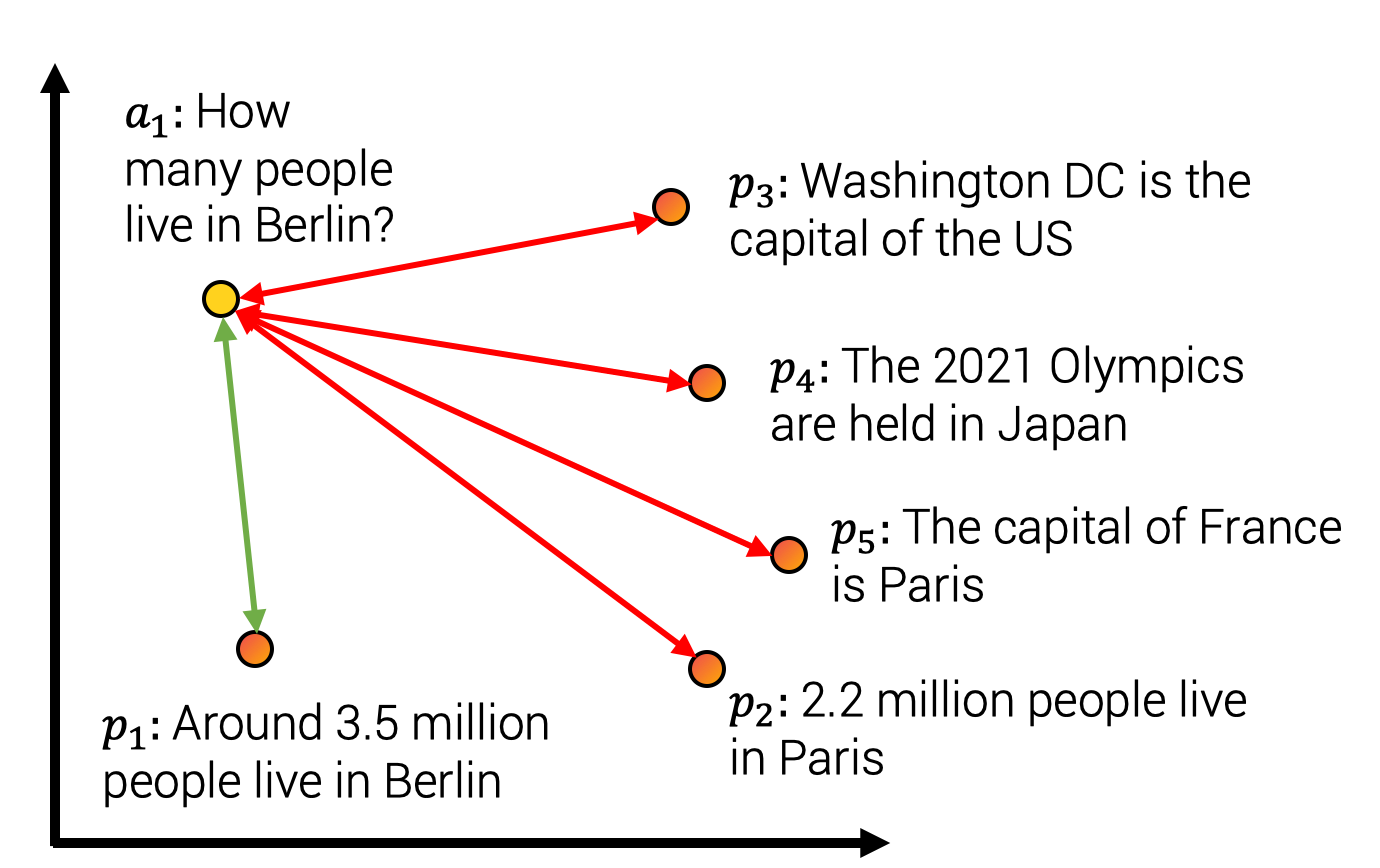
\includegraphics[width=10cm]{images/contrastive_1.png}
	\caption[Contrastive learning]{Illustration of the contrastive learning setup. The model is trained to associate an anchor sentence with another one that is semantically related. The notion of semantic relation depends on the nature of the pair. Our example aims to link the correct answer to a given question. City capitals are the subject of all these sentences, but only one is the correct answer.}
	\labfig{contrastive}
\end{figure}

As in other contrastive methods detailed in \refsec{training:self-supervised}, we build negative pairs by considering other samples from the batch. Given a batch of $n$ training samples, the model optimizes the following loss function:

\begin{equation}
    \mathcal{L} = -\frac{1}{n}\sum_{i=1}^n\frac{e^{c(a_i. p_i)}}{\sum_j e^{c(a_i. p_j)}}    
\end{equation}

Where $c$ is a \textit{critic function}, which measures the distance between two sentence embeddings $(a, p)$.\sidenote{A set of possible critics is presented in \cite{tschannen_19} Most functions are either the cosine similarity or the dot product operator. The cosine similarity has the nice advantage of presenting the highest similarity to itself since $cos(a, a) =1$. While with the dot-product other vectors can have higher similarities: $dot(a, a) < dot (a, b)$.}.

%We illustrate the training objective in \reffig{contrastive-2}.

% \begin{figure}[htb!]
% 	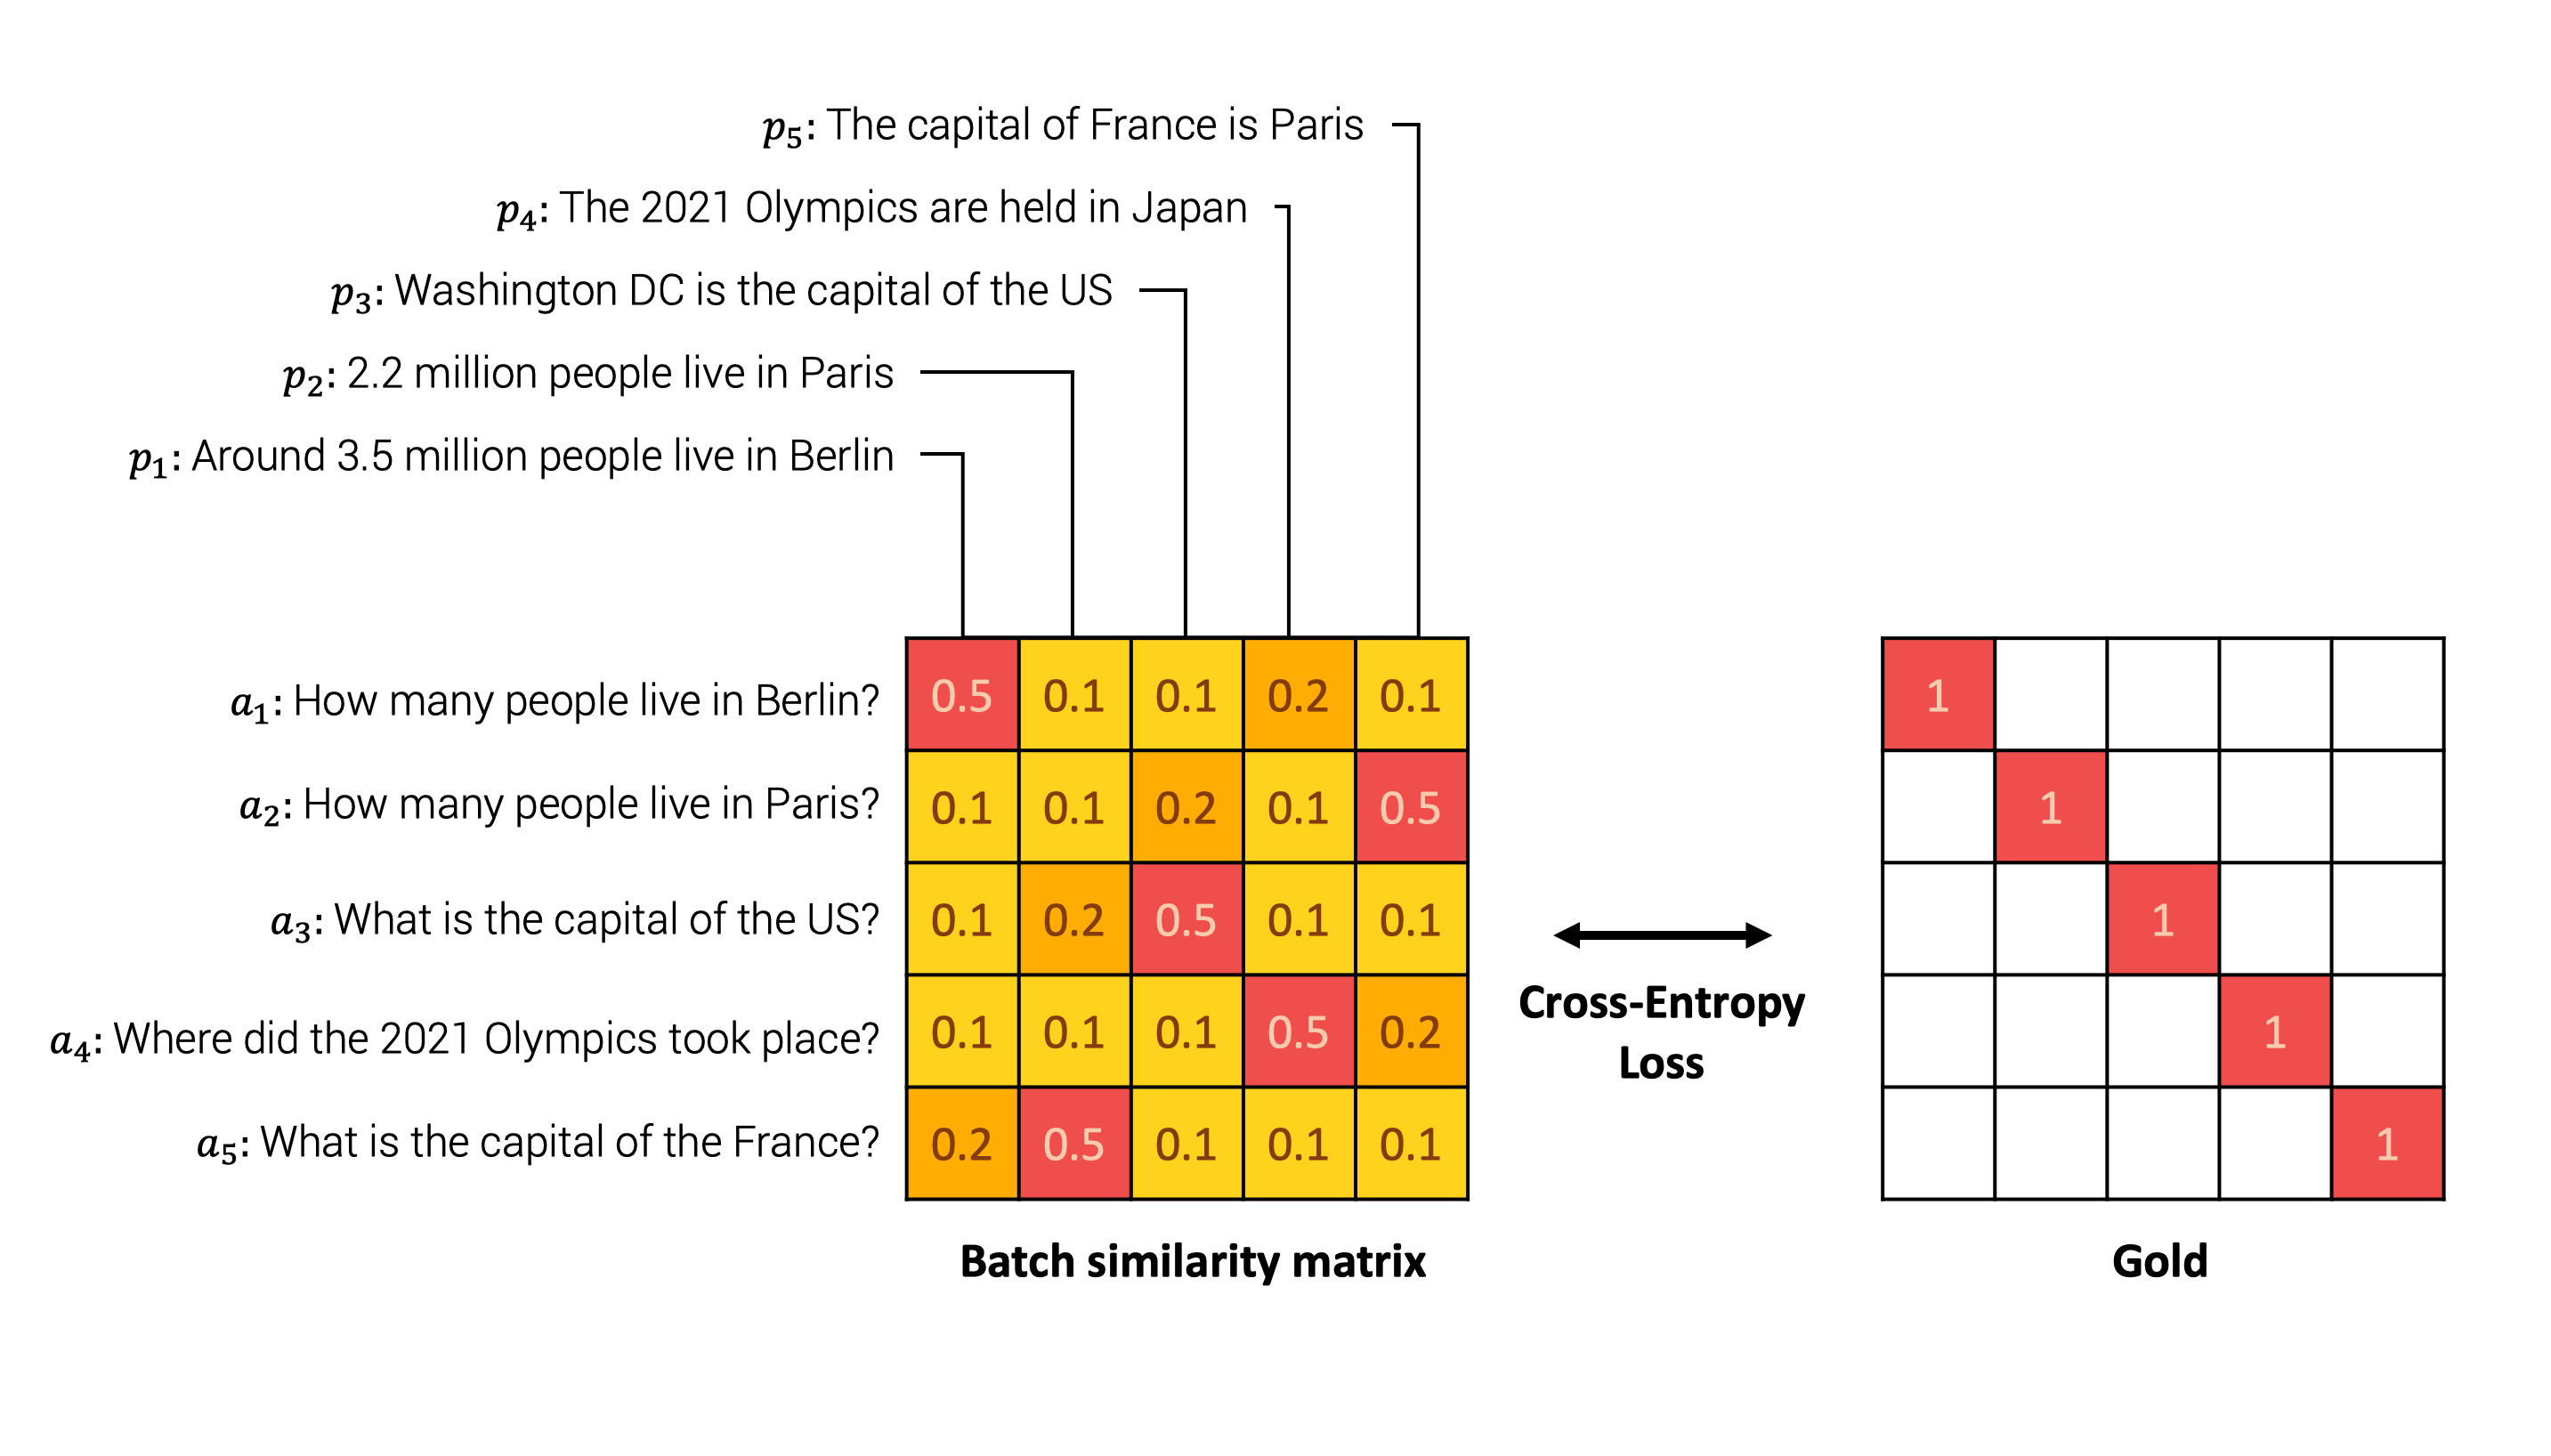
\includegraphics[width=10cm]{images/contrastive_2.png}
% 	\caption[Contrastive learning]{Illustration of the contrastive learning objective.}
% 	\labfig{contrastive-2}
% \end{figure}

\subsection{Construction of the dataset}
\labsec{1B:dataset}

The contrastive training method supposes to build a dataset such that each sample $x$ is combined with another sample $x^+$, which is somehow \textit{close} and negative samples $s^-_1 \cdots s^-_K$, which are not related. In \refch{structure-scale}, we constructed positive pairs by simply associating context sentences and negative by considering non-context sentences. Therefore, we only needed a corpus of raw text for which the sentence order is preserved to train our model. In this experiment, we adopt a more refined approach. Instead of raw text, we extract sentences from specific mediums such as internet forums or manually labeled datasets. Indeed, as detailed in \refsec{1B:batches}, a better selection of negative samples may drastically increase the results.

As with other attempts to scale model size \parencite{liu_2019, radford_2019, brown_20}, we also aim to scale the dataset size. While we use a 40M sentences dataset for \textcite{simoulin_2021a}, here, we aim to gather a dataset of 1B sentence pairs. The task is far from trivial as we need to constitute a dataset with sentence pairs $(a_i, p_i)$ such that sentences from the pair have a close meaning. We constitute pairs by using  medium and documents specific structure such as (query, answer-passage), (question, duplicate\_question), (paper title, cited paper title). We do not build new datasets but instead rely on existing work and aggregat many existing datasets enumerated in \reftab{tab:1B:dataset}.

The majority of the datasets is built out of Reddit comments. Reddit website aggregates news and lets users post links and discuss through threads. We use scripts from PolyAI to generate tuples given the first comment for each response.\sidenote{\url{https://github.com/PolyAI-LDN/conversational-datasets/tree/master/reddit}} We use the same filters as \textcite{henderson_2019} and filter out samples with more than 128 characters or fewer than 9 characters. I personally took care of this data collection operation.

\begin{table*}[!htb]
\centering
\footnotesize
\begin{tabularx}{16cm}{@{}lp{4.5cm}Y@{} }
\toprule
\textbf{Dataset} & \textbf{Reference} & \textbf{Number of training pairs} \\
\midrule
\midrule 
\href{https://github.com/PolyAI-LDN/conversational-datasets/tree/master/reddit}{Reddit Comments} (2015-2018) & \textcite{henderson_19} & \num{726484430} \\
\href{https://github.com/allenai/s2orc}{S2ORC} citation pairs (abstracts) & \textcite{lo_20} & \num{116288806} \\
\href{https://github.com/afader/oqa\#wikianswers-corpus}{WikiAnswers} duplicate question pairs & \textcite{fader_14} & \num{77427422} \\
\href{https://github.com/facebookresearch/PAQ}{PAQ} (question. answer) pairs & \textcite{lewis_21} & \num{64371441} \\
\href{https://github.com/allenai/s2orc}{S2ORC} citation pairs (titles) & \textcite{lo_20} & \num{52603982} \\
\href{https://github.com/allenai/s2orc}{S2ORC} (title. abstract) & \textcite{lo_20} & \num{41769185} \\
\href{https://huggingface.co/datasets/flax-sentence-embeddings/stackexchange_xml}{Stack Exchange} (title. body) pairs & - & \num{25316456} \\
\href{https://microsoft.github.io/msmarco/}{MS MARCO} triplets & \textcite{craswell_21} & \num{9144553} \\
\href{https://github.com/allenai/gooaq}{GOOAQ} & \textcite{khashabi_21} & \num{3012496} \\
\href{https://www.kaggle.com/soumikrakshit/yahoo-answers-dataset}{Yahoo Answers} (title. answer) & \textcite{zhang_15} & \num{1198260} \\
\href{https://huggingface.co/datasets/code_search_net}{Code Search} & - & \num{1151414} \\
\href{https://cocodataset.org/\#home}{COCO} image captions & \textcite{lin_14} & \num{828395} \\
\href{https://github.com/allenai/specter}{SPECTER} citation triplets & \textcite{cohan_20} & \num{684100} \\
\href{https://www.kaggle.com/soumikrakshit/yahoo-answers-dataset}{Yahoo Answers} (question. answer) & \textcite{zhang_15} & \num{681164} \\
\href{https://www.kaggle.com/soumikrakshit/yahoo-answers-dataset}{Yahoo Answers} (title. question) & \textcite{zhang_15} & \num{659896} \\
\href{https://huggingface.co/datasets/search_qa}{SearchQA} & \textcite{dunn_17} & \num{582261} \\
\href{https://huggingface.co/datasets/eli5}{Eli5} & \textcite{fan_19} & \num{325475} \\
\href{https://shannon.cs.illinois.edu/DenotationGraph/}{Flickr 30k} & \textcite{young_14} & \num{317695} \\
\href{https://huggingface.co/datasets/flax-sentence-embeddings/stackexchange_xml}{Stack Exchange} duplicate questions (titles) & - & \num{304525} \\
AllNLI (\href{https://nlp.stanford.edu/projects/snli/}{SNLI} and \href{https://cims.nyu.edu/~sbowman/multinli/}{MultiNLI}) & \textcite{bowman_15, williams_18b} & \num{277230} \\
\href{https://huggingface.co/datasets/flax-sentence-embeddings/stackexchange_xml}{Stack Exchange} duplicate questions (bodies) & - & \num{250519} \\
\href{https://huggingface.co/datasets/flax-sentence-embeddings/stackexchange_xml}{Stack Exchange} duplicate questions (titles and bodies) & - & \num{250460} \\
\href{https://github.com/google-research-datasets/sentence-compression}{Sentence Compression} & \textcite{filippova_13} & \num{180000} \\
\href{https://github.com/pvl/wikihow_pairs_dataset}{Wikihow} & \textcite{koupaee_18} & \num{128542} \\
\href{https://github.com/chridey/altlex/}{Altlex} & \textcite{hidey_16} & \num{112696} \\
\href{https://quoradata.quora.com/First-Quora-Dataset-Release-Question-Pairs}{Quora Question Triplets} & - & \num{103663} \\
\href{https://cs.pomona.edu/~dkauchak/simplification/}{Simple Wikipedia} & \textcite{coster_11} & \num{102225} \\
\href{https://ai.google.com/research/NaturalQuestions}{Natural Questions (NQ)} & \textcite{kwiatkowski_19} & \num{100231} \\
\href{https://rajpurkar.github.io/SQuAD-explorer/}{SQuAD2.0} & \textcite{drajpurkar_18} & \num{87599} \\
\href{https://huggingface.co/datasets/trivia_qa}{TriviaQA} & - & \num{73346} \\
\midrule
\textbf{Total} & & \textbf{\num{1124818467}} \\
\bottomrule
\end{tabularx}
\caption{1 billion sentence pairs dataset. We use already existing datasets accessible in open source or for which the raw data and pre-processing scripts were available. For each sub-dataset, we provide the link to the available resources (existing dataset or pre-processing scripts).}
\labtab{tab:1B:dataset}
\end{table*}

\subsection{Construction of the mini batches}
\labsec{1B:batches}

When building models. the selection of pairs forming a batch is crucial. We present here our strategy to constitute mini-batches and the impact it may have on the resulting embeddings.
% Here we examine the batch characteristics and their impact on the embeddings.

\paragraph{Batch size} The Quickthought method detailed in \refsec{training:self-supervised} uses a rather important batch size of 400. In fact, studies show that the more large the batch, the better the performances  \parencite{chen_20a, qu_21}. This trend is illustrated \reffig{batch-size} extracted from \textcite{qu_21}. Yet, too important batch size may decrease the results (the same asymptotic phenomenon is observed in \textcite{chen_20a}). We benefited from efficient hardware infrastructure to run the project: 7 TPUs v3-8, as well as guidance from Google’s Flax, JAX, and Cloud team members about efficient deep learning frameworks. We use the largest batch size that our hardware could fit, in our case, 64.

\begin{figure}[htb!]
	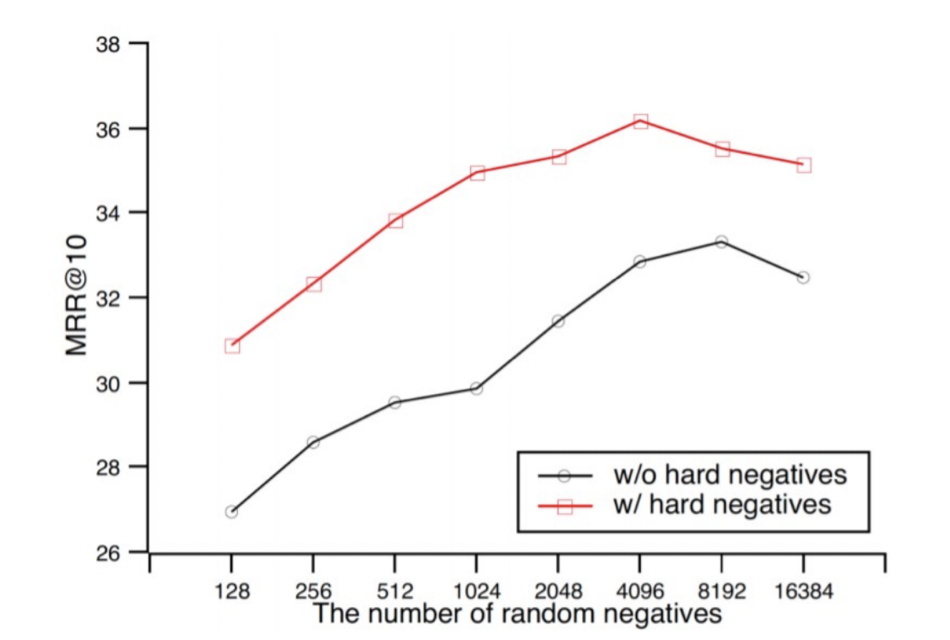
\includegraphics[width=10cm]{images/batch-size.png}
	\caption[Batch size]{Influence from the batch size and selection of hard negative on downstream evaluation. The figure is extracted from \textcite{qu_21}.}
	\labfig{batch-size}
\end{figure}

\paragraph{Hard Negatives} We may build batches by uniformly selecting samples from the training data. Yet, as detailed in \textcite{robinson_21} or \textcite{qu_21}. the selection of "good negative examples" significantly impacts the training process. The impact of hard negative is illustrated in \reffig{batch-size}.
Hard negative examples should not correspond to the anchor point but still, be difficult to distinguish from the correct associations. 
% Hard negatives are sample $p_j$. which are hard to distinguish from $p_i$. 
In our example, it could be the pairs « What is the capital of France? » and « What is the capital of the US? » which have a close semantic content and requires precisely understanding the full sentence to be answered correctly. On the contrary, the samples « What is the capital of France? » and «How many Star Wars movies are there?» are less difficult to distinguish since they do not refer to the same topic.

\paragraph{Cross dataset batches} In our case, the dataset is a concatenation of several sub-datasets (\reftab{tab:1B:dataset}). Each sub-dataset is built on distinct topics, domains, or semantic relations in the pair. We want to avoid the case where our model learns disjoint embedding spaces for each sub-dataset. On the other hand, mixing all sub-datasets in the same batch may deteriorate the hard negative proportion as samples issued from two sub-datasets should be easy to differentiate. To address both requirements, we build batches from the mix of only two sub-datasets. We aim, therefore, to learn a global structure between topics and not only a local structure within a topic while not deteriorating the proportion of hard negatives.

\subsection{Evaluation}
\labsec{scale:evaluation}

As detailed in \refsec{survey:downstream}, sentence embeddings are traditionally evaluated on the SentEval benchmark. To compare the embeddings with models developed in previous sections, we, therefore, evaluate our encoders on SentEval. However, as detailed in the same section, the benchmark suffers from practical limitations or biases. For this project, we, therefore, used SEB (Sentence Embedding Benchmark), a dedicated benchmark to compare our models.\sidenote{\url{https://github.com/nreimers/se-benchmark}} The SEB benchmark aggregates multiple general-purpose sentence evaluation tasks. The tasks, detailed below, are formatted as binary classification, clustering, reranking, retrieval, and semantic textual similarity (STS). All tasks use the embeddings as features and compare them using similarity metrics. Most importantly, they do not require the training of additional classifiers.

\paragraph{Binary classification} aims at predicting a binary relation between a pair of sentences. It computes the cosine similarity between every pair of sentences. We then classify the sentence pairs by comparing their similarity score to a given threshold. We set the threshold to ensure the best score on the development set. The task includes identifying paraphrases from LanguageNet, a collection of sentences from Twitter linked through shared URLs \sidenote{\url{https://languagenet.github.io/}} or the SemEval-2015 Task 1,\sidenote{\url{https://alt.qcri.org/semeval2015/task1/}} and identifying duplicated questions.\sidenote{\url{https://www.aclweb.org/anthology/D18-1131/}} We measure the performances using the average precision (AP).\sidenote{The average precision (AP) has values between 0 and 1 (higher is better). AP is defined as $\sum_n(R_n-R_{n-1})P_n$ with $P_n$ and $R_n$ are the precision and recall at the nth threshold. \url{https://scikit-learn.org/stable/modules/generated/sklearn.metrics.average_precision_score.html}}

\paragraph{Clustering} organizes documents into semantically consistent groups. We use data from web forums and newsgroups, which organizes posts given their topics. We use embeddings as features for K-Means clustering and evaluation using the V-measure.\sidenote{The V-measure evaluates the quality of a clustering given the ground truth labels. The score has positive values between 0 and 1, with higher values indicating better results. The V-measure is the harmonic mean between homogeneity and completeness. Homogeneity evaluates if each cluster contains only members of a single class. Completeness determines if all members of a class are assigned to the same cluster. \url{https://scikit-learn.org/stable/modules/generated/sklearn.metrics.v_measure_score.html}} The clustering task includes the 20Newsgroups,\sidenote{\url{https://scikit-learn.org/0.19/datasets/twenty_newsgroups.html}} and clustering threads from StackExchange and Reddit. 

\paragraph{Retrieval} aims at retrieving documents from a corpus that match the semantic content of a given query. We use datasets scraped from web forums and question-answering websites. On such platforms, experienced users can flag a question as a duplicate if it has already been answered elsewhere. We use these annotations to associate a given question to a list (of variable size) of semantically equivalent formulations. Given the embedding of a query, we compute the cosine similarity with other questions from the dataset and retrieve the top-$k$ most similar ones (by default, we use $k=10$). We then compare our predicted list with the related questions using the Mean average precision (MAP@100). The task includes CQADupStack, a dataset with duplicate question information from StackExchange subforums\sidenote{\url{http://nlp.cis.unimelb.edu.au/resources/cqadupstack/}} and the Quora Question Pairs dataset.\sidenote{\url{https://quoradata.quora.com/First-Quora-Dataset-Release-Question-Pairs}}
%  the Mean Reciprocal Rank (MRR) or 

\paragraph{Reranking} ranks a list of documents given their semantic similarity with a given query. In our setup, the task takes a query and a fixed-length list of documents as input. Each document in the list is either "similar" or "non-similar" to the query. We compute the cosine similarity between the embedding of the query and each document and sort them in decreasing order. We then compare the sorted list with the document ordered as similar first, followed by non-similar. We also use mean average precision to measure the quality of the ranking. As in the retrieval task, data are collected from web forums but with a different format and labeling process. We use a collection of questions taken from AskUbuntu.com 2014 corpus dump.\sidenote{\url{https://github.com/taolei87/askubuntu}} SciDocs. which consider scientific papers as related based on their inter citations \sidenote{\url{https://allenai.org/data/scidocs}} and the Stack Overflow Duplicate Questions Task.\sidenote{\url{https://www.microsoft.com/en-us/research/uploads/prod/2019/03/nl4se18LinkSO.pdf}}

\paragraph{Semantic Textual Similarity (STS)} measures the semantic similarity between two sentences. Annotators assign a similarity score for pair of sentences, ranging from 0 for no overlap to 5 for meaning equivalence. The annotation doesn't require formal linguistic expertise. Performance compares the correlation between predicted scores and human judgments with Pearson correlation. The predicted scores directly measure the cosine similarity between two sentence pairs and compare it with human gold annotations (scaled between 0 and 1). The evaluation datasets include the STSBenchmark\sidenote{\url{http://ixa2.si.ehu.eus/stswiki/index.php/STSbenchmark}} which includes datasets used for the SemEval task from 2012 to 2017. the SICK-R task (already introduced in \refsec{sts}) and BIOSSES \sidenote{\url{https://tabilab.cmpe.boun.edu.tr/BIOSSES/DataSet.html}} which comprises 100 sentence pairs from the biomedical field.

% \begin{table}[ht!]
% \begin{center}
% \small
% {\renewcommand{\arraystretch}{1.25}
% \begin{tabular}{|c|p{0.88\linewidth}|}
% \hline
% \multirow{4}{*}{5}& \emph{The two sentences are completely equivalent. as they mean the same thing.}\\
% \cline{2-2}
% & The bird is bathing in the sink. \newline Birdie is washing itself in the water basin. \\
% \hline
% \multirow{4}{*}{4}  & \emph{The two sentences are mostly equivalent. but some {\it unimportant} details differ.}\\
% \cline{2-2}
% & Two boys on a couch are playing video games. \newline Two boys are playing a video game. \\
% \hline
% \multirow{4}{*}{3} & \emph{The two sentences are roughly equivalent. but some {\it important information} differs/missing.}\\
% \cline{2-2}
% & John said he is considered a witness but not a suspect. \newline ``He is not a suspect anymore.'' John said.  \\
% \hline
% \multirow{4}{*}{2} & \emph{The two sentences are not equivalent. but share some details.}\\
% \cline{2-2}
% & They flew out of the nest in groups. \newline They flew into the nest together. \\
% \hline
% \multirow{4}{*}{1} & \emph{The two sentences are not equivalent. but are on the same topic.}\\
% \cline{2-2}
% & The woman is playing the violin. \newline The young lady enjoys listening to the guitar. \\
% \hline
% \multirow{4}{*}{0} & \emph{The two sentences are completely dissimilar.}\\
% \cline{2-2}
% & The black dog is running through the snow. \newline A race car driver is driving his car through the mud. \\
% \hline
% \end{tabular}
% }
% \end{center}
% \caption{Similarity scores with explanations and English examples. The table is exctracted from \textcite{cer_17}.}
% \label{fig:annotationcore}
% \end{table}

\section{Experiments}
\labsec{scale:experiments}

We fine-tune existing pre-trained models with our contrastive learning objective. As a sentence representation, we take the mean of every token hidden state from transformer models. We applied 500 warm-up steps and use a batch size of 64 if not explicitly specified otherwise. We create 20 general-purpose sentence transformers models such as Mini-LM \parencite{wang_20a}. RoBERTa \parencite{liu_2019}. DistilRoBERTa. a distilled version of the RoBERTa-base model following the same training procedure as DistilBERT \parencite{sanh_19}. and MPNet \parencite{song_20}.\sidenote{All models created during the challenge are available as open-source contributions in our HuggingFace repository \url{https://huggingface.co/flax-sentence-embeddings}.} The challenge was limited in time, and we could not extensively train all models with the same number of steps. We train RoBertA-large and MPNet-base for 400k steps. Mini-LM-12 for 540 steps. RoBERTa-distill-base for 920 steps and Mini-LM-6 for \numprint{1000} steps. Yet, models may therefore not be directly compared.



\paragraph{Analysis of the pre-training} We evaluate all our models on the Sentence Embedding Benchmark (SEB) detailed in \refsec{scale:evaluation} and SentEval benchmark introduced in \refsec{survey:downstream}. \reftab{scale:seb-senteval} reports the mean score for each model on both benchmarks. For each model, we report the score for the raw model and for the model further tuned with our additional contrastive pre-training.

\begin{table*}[!htb]
\centering
\small
\begin{tabularx}{16cm}{@{}lYYYYY@{} }
\toprule
&  & \multicolumn{2}{c}{\textbf{SentEval}} & \multicolumn{2}{c}{\textbf{SEB}}\\
\textbf{Model} & \textbf{\# parameters} & w/o contrastive pre-training & w/ contrastive pre-training & w/o contrastive pre-training & w/ contrastive pre-training\\
\midrule
\midrule 
\href{https://huggingface.co/flax-sentence-embeddings/all_datasets_v4_MiniLM-L6}{Mini-LM-6} & 22.7M & 80.6 & 83.5 & 42.0 & 68.1 \\
\href{https://huggingface.co/flax-sentence-embeddings/all_datasets_v4_MiniLM-L12}{Mini-LM-12} & 33.4M & 81.7 & 84.8 & 40.7 & 68.6 \\
\href{https://huggingface.co/flax-sentence-embeddings/all_datasets_v3_distilroberta-base}{DistilRoBERTa} & 82.1M & 83.5 & 86.0 & 44.9 & 68.7 \\
\href{https://huggingface.co/flax-sentence-embeddings/all_datasets_v4_mpnet-base}{MPNet-base} & 109.5M & \textbf{83.5} & \textbf{87.4} & 41.6 & 69.5 \\
\href{https://huggingface.co/flax-sentence-embeddings/all_datasets_v3_roberta-large}{RoBERTa-large} & 355.4M & 81.7 & 87.3 & \textbf{45.3} & \textbf{70.0} \\
\bottomrule
\end{tabularx}
\caption{\labtab{scale:seb-senteval} Evaluation on SentEval and SEB. We report the mean score over all tasks from the benchmark. We compare models pre-trained with and without our contrastive procedure. We report the best results for each category in \textbf{bold}.}
\end{table*}

In general, transformer models with a higher number of parameters reach higher scores. Yet, we observe asymptotic behavior for this trend. The RoBERTa-large model reaches performances similar to MPNet-base despite having 3 times more parameters. Moreover, on both benchmarks, the contrastive pre-training procedure has an important impact. Model performances increase up to 5.6 points on SentEval and more than 20 points on SEB. This confirms the relevance of the procedure for training sentence encoders with transformer architectures. Finally, we observe less disparity between models on the SEB benchmarks for which all scores are very close. 

\paragraph{Sentence Embedding Benchmark (SEB)} \reftab{scale:seb} reports the detailed evaluation of our models on SEB. The results are more difficult to interpret. While larger models tend in general to perform better, no model seems to consistently outperform others. It is also difficult to identify specifics models behavior across task classes.

\setlength\tabcolsep{2pt} % default value: 6pt
\begin{table*}[!htb]
\footnotesize
\centering {
\begin{tabularx}{16cm}{@{}l Y Y Y | Y Y Y | Y Y | Y Y Y | Y Y Y@{}}
\toprule
& \multicolumn{3}{c}{\textbf{Binary Classification}} & \multicolumn{3}{c}{\textbf{Clustering}} & \multicolumn{2}{c}{\textbf{Retrieval}} & \multicolumn{3}{c}{\textbf{Re-ranking}} & \multicolumn{3}{c}{\textbf{STS}}\\
& {\tiny\textbf{Sprint}} & {\tiny\textbf{Twitter}} & {\tiny\textbf{SemEval}} & {\tiny\textbf{20 News Groups}} & {\tiny\textbf{Stack Exchange}} & {\tiny\textbf{Reddit}} & {\tiny\textbf{CQA}} & {\tiny\textbf{Quora}} & {\tiny\textbf{Ask Ubuntu}} & {\tiny\textbf{Sci Docs}} & {\tiny\textbf{Stack Overflow}} & {\tiny\textbf{SICK-R}} & {\tiny\textbf{STS}} & {\tiny\textbf{BIOSSES}}\\\midrule
\midrule
\href{https://huggingface.co/flax-sentence-embeddings/all_datasets_v4_MiniLM-L6}{Mini-LM-6} & \textbf{94.6} & 84.7 & 67.9 & 46.2 & 54.4 & 50.2 & 28.6 & 84.9 & 63.5 & 87.1 & 50.8 & 77.2 & 82.0 & 81.6 \\
\href{https://huggingface.co/flax-sentence-embeddings/all_datasets_v4_MiniLM-L12}{Mini-LM-12} & 92.6 & 84.8 & 70.0 & 46.9 & 52.4 & 50.6 & 29.4 & \textbf{85.1} & 64.1 & 87.2 & 51.5 & 78.9 & 83.1 & 83.6 \\
\href{https://huggingface.co/flax-sentence-embeddings/all_datasets_v3_distilroberta-base}{DistilRoBERTa} & 46.8 & 65.2 & \textbf{83.3} & 30.5 & 83.4 & 53.1 & 80.1 & 82.4 & 87.8 & \textbf{93.8} & 48.7 & 51.4 & 71.1 & 84.0 \\
\href{https://huggingface.co/flax-sentence-embeddings/all_datasets_v4_mpnet-base}{MPNet-base} & 90.2 & \textbf{85.1} & 73.9 & \textbf{49.8} & 52.9 & 54.1 & 31.8 & 84.7 & 65.9 & 88.6 & 52.0 & \textbf{80.5} & \textbf{83.4} & 80.4 \\
\href{https://huggingface.co/flax-sentence-embeddings/all_datasets_v3_roberta-large}{RoBERTa} & 49.4 & 66.8 & 82.5 & 32.8 & \textbf{83.4} & \textbf{55.6} & \textbf{81.4} & 83.5 & \textbf{88.7} & 92.1 & \textbf{52.5} & 52.2 & 75.3 & \textbf{84.5} \\
\bottomrule
\end{tabularx}}
\caption{\labtab{scale:seb} Detailed results on the Sentence Embeddings Benchmark (SEB). All models are further pre-trained using our contrastive objective on our 1 billion sentences corpus. The best results in each section are shown in \textbf{bold}. We report the mean average precision (AP) for binary prediction and retrieval tasks, the V-measure for clustering tasks, and the Spearman rank correlation for semantic textual similarity task (STS). For each task, we report the best score obtained with cosine, euclidean, and Manhatten distance. We report all metrics by convention as $\times 100$. We show the best results in \textbf{bold}.}
\end{table*}
\setlength\tabcolsep{6pt} % default value: 6pt

\paragraph{SentEval} Finally, we aim to compare our transformer models with previously presented encoders from \refch{structure-scale}. We present the detailed results on SentEval in \reftab{scale:senteval}. We divide results given encoder architecture: LSTM and transformer-based models. 

\begin{table*}[!htb]
\footnotesize
% \begin{minipage}{\textwidth}
\centering {
\begin{tabularx}{16cm}{@{}l c | Y Y Y Y Y Y Y Y Y Y Y @{}}
\toprule
\multirow{2}{*}{\textbf{Model}} & \multirow{2}{*}{\textbf{Dim}} & \multirow{2}{*}{\textbf{Avg.}} & \multirow{2}{*}{\textbf{MR}} & \multirow{2}{*}{\textbf{CR}} & \multirow{2}{*}{\textbf{SUBJ}} & \multirow{2}{*}{\textbf{MPQA}} & \multirow{2}{*}{\textbf{TREC}} &  \multicolumn{2}{c}{\textbf{MRPC}} &  \multicolumn{3}{c}{\textbf{SICK-R}}\\%\cmidrule(r){9-10} \cmidrule(r){11-13}
 &  &  &  &  &  &  &  & \textbf{Acc} & \textbf{F1} & \textbf{$r$} & \textbf{$\rho$} & \textbf{MSE}\\\midrule
\multicolumn{13}{c}{\textit{Recurrent models}} \\\midrule
FastSent & $\leq500$ & --- & 70.8 & 78.4 & 88.7 & 80.6 & 76.8 & 72.2 & 80.3 & --- & --- & ---\\
% FastSent + AE & $\leq500$ & 2 & 71.8 & 76.7 & 88.8 & 81.5 & 80.4 & 71.2 & 79.1 & --- & --- & ---\\
Skipthought & \numprint{4800} & 83.8 & 76.5 & 80.1 & 93.6 & 87.1 & 92.2 & 73.0 & 82.0 & 85.8 & 79.2 & 26.9\\
% Skipthought + LN & \numprint{4800} & 672 & 79.4 & 83.1 & 93.7 & 89.3 & --- & --- & --- & 85.8 & 78.8 & 27.0\\
Quickthought & \numprint{4800} & \textbf{86.1} & 80.4 & 85.2 & 93.9 & 89.4 & 92.8 & 76.9 & 84.0 & 86.8 & 80.1 & 25.6\\
InferSent & \numprint{4096} & --- & \textbf{81.1} & \textbf{86.3} & 92.4 & 90.2 & 88.2 & 76.2 & 83.1 & \textbf{\underline{88.4}} & --- & ---\\
% DisSent Books 5 & \numprint{4096} & --- & 80.2 & 85.4 & 93.2 & 90.2 & 91.2 & 76.1 & --- & 84.5 & --- & ---\\
DisSent & \numprint{4096} & --- & 79.8 & 85.0 & 93.4 & \textbf{\underline{90.5}} & \textbf{93.0} & 76.1 & --- & 85.4 & --- & ---\\
\textsc{Dep}. \textsc{Seq}$^\dagger$ & \numprint{4800} & 85.3 & 79.7 & 82.2 & 94.4 & 88.6 & 91.0 & \textbf{\underline{77.9}} & \textbf{\underline{84.4}} & 86.6 & 79.8 & 25.5\\
\textsc{Dep}. \textsc{Const}$^\dagger$ & \numprint{4800} & 86.0 & 80.7 & 83.6 & \textbf{94.9} & 89.2 & 92.6 & 76.8 & 83.6 & 87.0 & \textbf{80.3} & \textbf{24.8}\\
\midrule\multicolumn{13}{c}{\textit{Transformers}} \\\midrule
\textsc{Bert}-base [CLS] & $768$ & --- & 78.7 & 84.9 & 94.2 & 88.2 & 91.4 & 71.1 & --- & 75.7$^\dagger$ & --- & ---\\
\textsc{Bert}-base [NLI] & $768$ & --- & 83.6 & \textbf{\underline{89.4}} & 94.4 & 89.9 & 89.6 & \textbf{76.0} & --- & 84.4$^\dagger$ & --- & ---\\
\href{https://huggingface.co/flax-sentence-embeddings/all_datasets_v4_MiniLM-L6}{Mini-LM-6}$^\dagger$ & $384$ & 83.5 & 76.1 & 82.0 & 92.2 & 87.4 & 90.2 & 72.3 & 80.9 & 86.5 & 79.9 & 25.6 \\
\href{https://huggingface.co/flax-sentence-embeddings/all_datasets_v4_MiniLM-L12}{Mini-LM-12}$^\dagger$ & $384$ & 84.8 & 77.9 & 84.3 & 92.3 & 88.4 & 91.8 & 73.2 & \textbf{82.1} & 87.1 & 80.9 & 24.7 \\
\href{https://huggingface.co/flax-sentence-embeddings/all_datasets_v3_distilroberta-base}{DistilRoBERTa}$^\dagger$ & $768$ & 86.0 & 80.8 & 86.2 & 93.4 & 87.6 & 94.8 & 73.5 & 80.9 & \textbf{87.8} & 82.3 & 23.4 \\
\href{https://huggingface.co/flax-sentence-embeddings/all_datasets_v4_mpnet-base}{MPNet-base}$^\dagger$ & $768$ & \textbf{\underline{87.5}} & 84.8 & 87.7 & 94.1 & 89.4 & 94.4 & 75.1 & 83.4 & 87.9 & 82.9 & \textbf{\underline{23.3}} \\
\href{https://huggingface.co/flax-sentence-embeddings/all_datasets_v3_roberta-large}{RoBERTa-large}$^\dagger$ & \numprint{1024} & 87.3 & \textbf{\underline{87.0}} & 88.6 & \textbf{\underline{95.0}} & \textbf{89.0} & \textbf{\underline{96.8}} & 74.0 & 80.6 & 83.7 & \textbf{\underline{83.9}} & 35.5 \\
\bottomrule
\end{tabularx}}
\caption{\labtab{scale:senteval} SentEval Task Results Using Fixed Sentence Encoder. $^\dagger$\ indicates models that we had to re-train. FastSent is reported from \textcite{hill_16}. Skipthoughts results from \textcite{kiros_15} Skipthoughts + LN which includes layer normalization method from \textcite{ba_16}. We considered the Quickthought results \cite{logeswaran_18} with a pre-training on the bookcorpus dataset. DisSent and Infersent are reported from \textcite{nie_19} and \textcite{conneau_17} respectively. Pre-trained transformers results are reported from \textcite{reimers_19}. Best results in each section are shown in \textbf{bold}. best results overall are \underline{underlined}. Performance for \textbf{SICK-R} results are reported by convention as $\rho \text{ and } r \times 100$.}
\end{table*}

We obtain state-of-the-art results on the benchmark, and transformer-based models outperform other architectures. On many tasks, we also outperform the approach proposed in \textcite{reimers_19}, which fine-tune \textsc{Bert} on natural language inference data. However, LSTM based models remain competitive on several tasks. Moreover, only transformers with the highest number of parameters outperform previous recurrent models. It is also important to stress that the setup is not directly comparable as transformer models are trained on datasets many orders of magnitude larger.

\section{Conclusion and future work}


% \bcomment{You might well comment that bigger is not necessarily better ? throwing more data is not the only solution:what explains your MRPC result it is better with a biased model trained on relatively less data}{or maybe that bigger is better but in which proportions ?}
% \bcomment{See my notes in the conclusion}{You might wish to conclude on these aspects, I find your MRPC results quite interesting to analyze in the conclusion with these respects}{}

In this section, we studied the extent to which scaling may improve sentence encoder performances. We adapt the standard contrastive pre-training method to train large transformer models on a large dataset. We obtain state-of-the-art results on sentence embedding benchmarks. We observe the importance of contrastive pre-training to achieve competitive results. In some proportion, it seems possible to balance linguistic insights and the refinement of the encoder architecture by just increasing the dataset and model size. 

However, it is important to stress that the setup is completely unbalanced and the comparison rather unfair regarding the infrastructure hardware, the data used for training, and the model size.

Finally, bigger is not necessarily better. Indeed, while large models outperform previous recurrent and structured approaches on average, this is not the case for every task. In particular for the MRPC task: the Microsoft Research Paraphrase Corpus contains \numprint{5801} sentence pairs, each hand-labeled with a binary judgment as to whether the pair constitutes a paraphrase. The sentences are mined from news clusters and includes a wide range of lexical as well as syntactic variations.


\setlength\tabcolsep{6pt} % default value: 6pt

% \setchapterimage[6cm]{seaside}
\setchapterstyle{kao}
\setchapterpreamble[u]{\margintoc}
\chapter{The first large incremental language model for French}
% using a generative objective
\labch{generative}

% \cleanchapterquote{\textup{[\,\dots]} le sujet s’éloigne du verbe et \textup{[\,\dots]} le complément vient se poser quelque part dans le vide.}{Samuel Beckett}{Malone meurt, 1951}
\cleanchapterquote{La nuit se faisait assez obscure, les étoiles semblaient dormir de temps à autre, cependant le peu de clarté qui me permit de marcher la nuit dans la chambre éveilla en moi une profonde pitié de ce que je faisais là, et cette peur de l'avenir me devint plus vive et plus aiguë.}{Automatic text generation}{$\text{GPT}_{fr}$-1B, 2021}

% \section{Training efficient sentence embedding models using structured encoders}
% \labsec{structure-scale}
% Previous sections examined the training of models by predicting relationships between sentences. Here, 

The previous section discussed enhancing large transformer language models using self-supervised objectives adapted for sentence embeddings. Our procedure reached state-of-the-art results on many downstream evaluation tasks. However, we did not perform the initial pre-training ourselves but instead used already pre-trained transformers for English. This section presents a quantitative evaluation of the effort required to pre-train such models in terms of data collection, computing infrastructure configuration, model development, and evaluation. To be as representative as possible of the process, we chose a language and architecture design for which relatively few resources
%french is usually said to be a well resourced language
were available. The section thus relates the pre-training of the first large incremental language model for French \parencite{simoulin_2021c}.

Auto-encoding models have already been developed in French, namely CamemBERT \parencite{martin_20} or FlauBERT \parencite{le_20a, le_20b}. However, to the best of our knowledge, this contribution is the first peer-reviewed to adapt pre-trained incremental transformers to French. In particular, we introduced a French version from the well-known GPT model \parencite{radford_2018, radford_2019, brown_20}. GPT, which stands for Generative Pre-trained Transformer, is an incremental language model developed by Open AI research laboratory\sidenote{\url{https://openai.com/}}. \bert and other models presented in the previous sections act as encoders, taking text as input and producing vector representations as output. On the contrary, GPT acts as a decoder, taking text as input and producing text as output. 
%rappeler ce qu'est GPT, et donner une spécification de ton modèle dans le chapitre, segmentation etc; contraster l'objectif avec celui de BERT etc histoire que le chapitre soit stand alone.
% Parler du défi pour entrainer ce type de model
%\bcomment{titre mal choisi}{Camembert et flaubert sont venus avant}

From a modeling point of view, \gpt is an incremental language model whose pre-training objective is relatively similar to the one from a n-gram language model already used 30 years ago. But while n-gram language models typically use a context size of 5 or fewer words, \gpt extends the context size to \numprint{1024} tokens. From a practical point of view, pre-training such a model is a superlative project, which is far from trivial. First, it requires large corpora of raw text—up to billion of tokens. Second, the analysis and evaluation of these models require access to relevant and rigorous benchmarks. Last but not least, pre-training also requires significant computing power. It requires distributing the training on multiple computing units across multiple computing nodes. Typically dozens of graphics processing unit (GPUs) or tensor processing units (TPUs) %\sidenote{\url{https://cloud.google.com/tpu}} 
operating for several days. In that regard, this work benefited from access to the IDRIS computing facilities through the allocation of 2020-AD011011823 allocated by GENCI. Our model was among the firsts to be trained on the super-computer Jean-Zay, less than a year after its inauguration in January 2020. Our contributions are the following:
\begin{itemize}
    \item We propose a corpus dedicated to the training of transformers language models in French. We detail the construction of this corpus in \refsec{generative:corpus} ;
    \item We train two models with a large number of parameters, which we release as open-source contributions\sidenote{\url{https://huggingface.co/asi/gpt-fr-cased-base}}. Hopefully, these models can be used in academic as well as industrial settings ;
    \item We replicate English evaluation benchmarks for French language models. This evaluation setup allows for the comparison of models and is detailed in \refsec{generative:evaluation}.
\end{itemize}

% We organize the section as follow: We first present the construction of the training and evaluation corpora (\refsec{generative:corpus}). We then detail the architecture and training setup in \refsec{generative:models}. Finally,  \refsec{generative:evaluation} examines our model abilities through several evaluation tests.

% In this case, we are mining a specific datasets with many sentence pairs. \bcomment{There are also methods for reconstructing a noised input, for example detecting masked words or predicting what the next word will be. The corpora required for such auto-encoding methods are more simple and only consist in individual documents.}{raw text ?}

% In this section, we introduce a French \bcomment{adaptation}{version} from the well-known \bcomment{GPT}{rappeler ce qu'est GPT, et donner une spécification de ton modèle dans le chapitre, segmentation etc; contraster l'objectif avec celui de BERT etc histoire que le chapitre soit stand alone} model. GPT relies on transformer pre-trained architectures, which profoundly transformed natural language processing methods. Such models are pre-trained using a self-supervised objective and are therefore specific to a given language. The model, equivalent to GPT-2 in English, contains more than 1 billion parameters. \bcomment{This work benefited from access to the IDRIS computing facilities through the allocation of 2020-AD011011823 allocated by GENCI.}{dire que ce modèle est un des premiers à avoir été entrainé sur l'IDRIS, mettre en avant dans le chapitre le coté infrastructure : calcul distribué, combien de noeuds, temps d'entrainement etc.}

% Although some models may exist in French, the majority is released in \bcomment{English}{cela vaudrait le coup d'inclure une section qui résume un peu ce qui change; est-il aussi facile de trouver les données ? commenter le zero-shot etc.} only.  


We organize the section as follow: \refsec{generative:incremental} first reviews the main characteristic of incremental models, their originality and main distinctions with standard encoders. \refsec{generative:corpus} presents the constitution of the pre-training corpora. We then detail the training and evaluation procedure in \refsec{generative:training} and \refsec{generative:evaluation}. Finally, we discuss the limits and ethical considerations in \refsec{generative:limits}.


%GPT achieves impressive language generation performances. 

% Within my laboratory, I led the project to train the first large language model in French \parencite{simoulin_2021c}. We obtained a dedicated computation grant on public French HPC computer Jean Zay. The model, equivalent to GPT-2 in English, contains more than 1 billion parameters. We built a dedicated training corpus and parallelized the training between multiple nodes and compute units. I am particularly proud of this project, as we contributed to the resources available in French. We released the model in Open-Source for research and business application purposes. 

%TODO il faut parler des embeddings de phrase de ces modèles et le relier à la problématique de la thèse

% This is, to the best of our knowledge, the first peer-reviewed contribution that \bcomment{adapts pre-trained generative transformers}{nope there are camembert and flaubert} to French. We adapt OpenAI GPT et GPT-2 \parencite{radford_2018, radford_2019} for French. Our contributions are the following:
% \begin{itemize}
%     \item We propose a corpus dedicated to the training of transformers language models in French. The construction of thus corpus is detailed in \refsec{generative:corpus} ;
%     \item We \acomment{trained} two models with a large number of parameters, which we released as open-source contributions\sidenote{\url{https://huggingface.co/asi/gpt-fr-cased-base}}. Hopefully, these models can be used in academic as well as industrial settings. We detailed the architecture of the models in \refsec{generative:models} ;
%     \item We replicate English evaluation benchmarks for French language models. This evaluation setup allows for the comparison of models and is detailed in \refsec{generative:evaluation}.
% \end{itemize}

\section{Auto-regressive language models}
\labsec{generative:incremental}
% rappeler ce qu'est GPT, et donner une spécification de ton modèle dans le chapitre, segmentation etc; contraster l'objectif avec celui de BERT etc histoire que le chapitre soit stand alone
% cela vaudrait le coup d'inclure une section qui résume un peu ce qui change; est-il aussi facile de trouver les données ? commenter le zero-shot etc.
% The model can address a large variety of tasks. In particular, the model may benefit from original configurations such as few-shot or zero-shot learning. In such configurations, it is possible to address tasks without any parameters fine-tuning.

% Assuming pre-training corpus consists of a sequence of tokens $U=\{u_1 \cdots u_T\}$, the model can finally be described simply according to the following equations:

As detailed in \refsec{architectures:transformers}, \gpt or \bert are based on transformer architectures. Both models take as input sequence of tokens\sidenote{Here we tokenize the input text using bytepair vocabulary encoding (BPE) with \numprint{50000} units \parencite{sennrich_16a}. This procedure allows for a relatively reduced vocabulary size while drastically reducing the number of tokens out of the vocabulary.} and encode them as the sum of a token and positional embeddings (\refeq{generative:embeddings}). Token embedding vectors are then transformed into so-called contextualized vectors through a series of $L$ transformer layers (\refeq{generative:layers-eq}).

\begin{align}
    h^0_t &= W_eu_t + W_p \quad \forall t \in \llbracket 1, T \rrbracket \labeq{generative:embeddings} \\
    h^n_t &= \mathsf{layer}(h^{n-1}_t) \quad \forall n \in \llbracket 1, L \rrbracket \labeq{generative:layers-eq}
\end{align}

With $\{u_1 \cdots u_T\}$ the sequence of input tokens, $L$ the number of layers, $W_e$ the embedding matrix, and $W_p$ the positional embedding matrix.

% \begin{gather}
% \begin{align}
%     & h_0^t = u^tW_e+W_p \labeq{generative:embeddings}\\
%     &h_i = \textrm{decoder\_layer}(h_{i-1}), \quad \forall i \in [1,n] \\
% \end{align}
% \end{gather}

Each layer in \refeq{generative:layers-eq} acts as a many-to-many encoder. \bert and its derivatives use so-called encoder layers: it computes contextualized representations given the right and left contexts \ie from the tokens immediately after and before the considered position. \gpt, however, relies on decoder layers: contextualized representations only depend on the left context, that is, tokens before the considered position. We illustrate this key distinction in \reffig{generative:self-attention-decoder}.

\begin{figure}[htbp]
\begin{center}
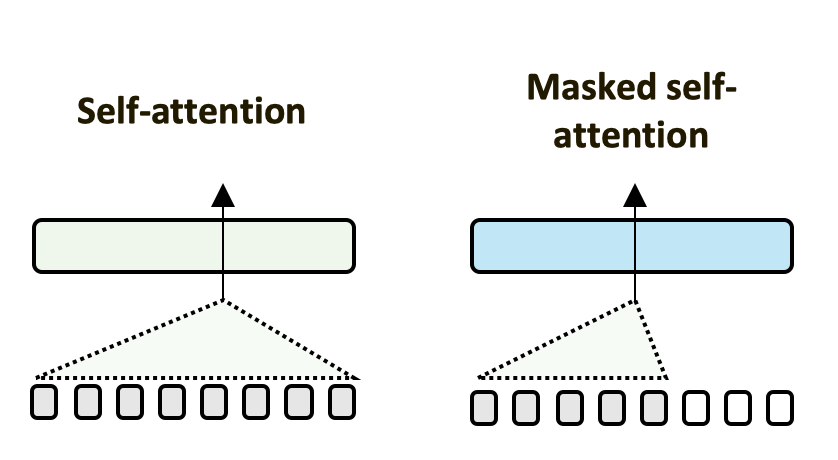
\includegraphics[width=8cm]{images/self-attention.png}
\end{center}
\caption{Illustration of the self-attention scope for encoding and decoding layers.}
\labfig{generative:self-attention-decoder}
\end{figure}

% and \bcomment{shares many similarities with \textsc{Bert}}{too fuzzy, which ones ?}. It consists in successive decoder layers. The main difference with \textsc{Bert} is that the multi attention-heads only focus on tokens preceding the considered position. \bcomment{too fuzzy }{introduce that earlier and with a cleaner formalization}

This difference in design has important implications for both architectures' training and inference setups. We detail such implications during the pre-training phase in \refsec{generative:autoregressive:pre-training} and during inference in \refsec{generative:autoregressive:inference}.


\subsection{Pre-training}
\labsec{generative:autoregressive:pre-training}

\bert and \gpt are pre-trained using a language model training objective: they associate a probability $P(u_1 \cdots u_T)$ to a sequence of tokens. We can decompose this sequence probability as the product of conditional probabilities for each token:

\begin{equation}
    P(u_1 \cdots u_T) = \prod_{t \in \llbracket 1, T \rrbracket} P\left(u_t \middle| U \right)
\end{equation}

With $U$ the context of $u_t, \forall t \in \llbracket 1, T \rrbracket$. Given the contextualized representations of each token from \refeq{generative:layers-eq}, we can compute the conditional probabilities associated with each token given \refeq{generative:token-proba}.

\begin{equation}
    P\left(u_t \middle| U \right) = \softmax(h_t^N W_e^T) \labeq{generative:token-proba} \\
    % \mathcal{L}(U) = \sum_i log P\left(u_{i} \middle| u_{i-k} \cdots u_{i-1}  ; \Theta\right)
\end{equation}

With $h_t^N$ the contextualized representation from the last layer of the token at index $t$. 

\bert relies on a bidirectional context to build representations. Each token contextualized representation is conditioned on every other tokens from the input, including himself, such that $P\left(u_t \middle| U \right) = P\left(u_t \middle| u_1 \cdots u_T \right)$. Since, a given token contextualized representation depends on the token itself, \bert uses a \textit{trick} for pre-training by replacing some tokens with a \texttt{[MASK]} in the input text. Thus, such tokens are "masked" and not used to build contextualized representations. The model is then trained to predict the original token at masked positions. 

\gpt only uses the left context to build token representations, such that $P\left(u_t \middle| U \right) = P\left(u_t \middle| u_1 \cdots u_{t-1} \right)$. Therefore, it is unnecessary to use such artifice. We only pre-train the model using a standard incremental language model objective: predicting the next token given the previous ones. Assuming the pre-training corpus $D$ consists of a collection of documents $d=\{u_1 \cdots u_T\}$\sidenote{To simplify the notations, we omit the document index such that we refer to the tokens of all documents as $\{u_1 \cdots u_T\}$ and not $\{u^{(d)}_1 \cdots u^{(d)}_T\}$.}, we optimize the \gpt parameters $\Theta$ to maximize the following log-likelihood:% $\mathcal{L}(U)= \sum_i log P\left(u_{i} \middle| u_{i-k} \cdots u_{i-1}  ; \Theta\right)$. 

\begin{equation}
    \mathcal{L}(D) = \sum_{d \in D}\sum_{i \in \llbracket 1, T \rrbracket} \log P\left(u_{i} \middle| u_{i-k} \cdots u_{i-1}  ; \Theta\right)
\end{equation}

With $k$ the context-size, and $U=\{u_{i-k} \cdots u_{i-1}\}$ the context of the token at position $i$.


\subsection{Inference}
\labsec{generative:autoregressive:inference}

\paragraph{Standard fine-tuning} Once the model is pre-trained, it is possible to fine-tune it on downstream tasks. Fine-tuning incrementally adjusts all model parameters to optimize the loss on a specific task. In such case, we take tokenized text as input $X = x_1 \cdots x_m$. We transform the input using our transformer into contextualized representations $h^N_1 \cdots x^N_m$ (\refeq{generative:gpt-std}). We then feed representations from the sequence to a dense layer with parameters $W^{(y)}$ followed by a softmax to predict the label $\hat{y}$ (\refeq{generative:softmax}). In the case of \bert, we usually use the first token $h^N_1$ of the sequence as input of the dense layer. For \gpt, we usually use the last token $h^N_m$. We seek to optimize a loss function comparing the true labels $y$ with the predictions $\hat{y}$ (\refeq{generative:loss}). 

% P\left(y \middle| x^1 \cdots x^m \right)
\begin{align}
    h_N^m &= \textrm{GPT}(x_1 \cdots x_m) \labeq{generative:gpt-std} \\
    \hat{y} &= \softmax(h_N^m W^{(y)}) \labeq{generative:softmax} \\
    \mathcal{L} &= \sum_{y \in Y} \mathcal{L}(\hat{y}, y) \labeq{generative:loss} 
\end{align}

On the one hand, when encoding a fixed-length text for downstream tasks, \gpt deprives itself of half of the contextualized information and thus usually reaches performances below \bert on many downstream tasks. On the other hand, since \gpt only uses the left context to build contextualized representations, it is a natural candidate for natural language generation. We illustrate this configuration in \reffig{generative:inference} (right sub-figure).

% \bcomment{Once the model is pre-trained, it is possible to use it like the standard transformers}{that is ?}. \bcomment{We add a specific layer to the task at the output of the model. We then adjust all the parameters incrementally (fine-tuning) given the task examples $x_1 \cdots x_m$ and their corresponding labels $y$. }{imbitable}

% To predict $y$, we pass this representation in a dense layer with parameters $W_y$ followed by a softmax: 
% $P\left(y \middle| x^1 \cdots x^m \right)=\textrm{softmax}(h_l^m W_y)$. We then try to maximize the cost function: $L(C)=logP\left(y \middle| x^1 \cdots x^m\right)$.
\paragraph{Generative tasks formatting} It is also possible to formalize the tasks to benefit from the generative characteristics of the model. Instead of predicting a probability distribution over the labels $y$, we can generate the labels $y$ directly in natural language. We transform the dataset into sequences $x_1 \cdots x_m [SEP] y$. We formalize each task as a language generation task. We fine-tune the model to "generate" the label $y$ in natural language, as the continuation of the input natural language sequence $x_1 \cdots x_m [SEP]$ (\refeq{generative:gpt-lm} and \refeq{generative:token-proba-m+1}). We then seek to optimize \gpt parameters $\Theta$ to maximize the cross-entropy between $\hat{y}$ and $y$ (\refeq{generative:cross-entropy}).

% P\left(y \middle| x^1 \cdots x^m\right)
\begin{align}
    h_{m+2}^N &= \textrm{GPT}(x_1 \cdots x_m [SEP]) \labeq{generative:gpt-lm} \\
    \hat{y} &= \softmax(h_{m+2}^N W_e^T) \labeq{generative:token-proba-m+1} \\
    \mathcal{L} &= y \log(\hat{y}) \labeq{generative:cross-entropy}
\end{align}

In this configuration, it is not necessary to modify the model's architecture or add any specific layer. We illustrate this configuration in \reffig{generative:inference} (left sub-figure).

\begin{figure}[!htb]
\begin{center}
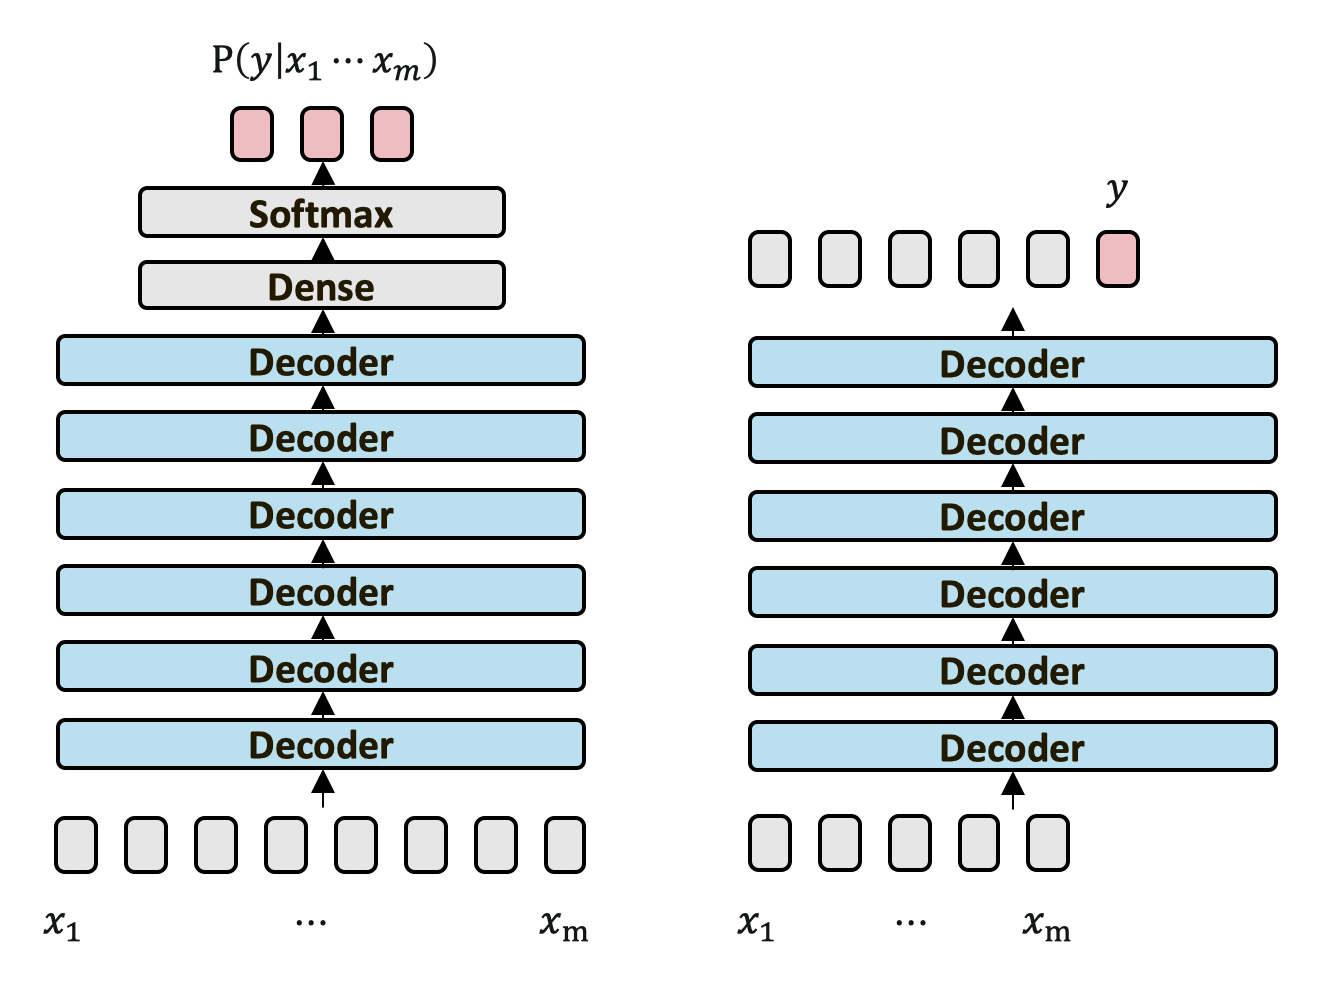
\includegraphics[width=10cm]{images/generative-2.png}
\end{center}
\caption{Configurations for incremental language models at inference. (left) standard configuration with dense and softmax layers (right) generative configuration for which the target is directly predicted as a sequence of words in natural language.}
\labfig{generative:inference}
\end{figure}

\paragraph{Few or zero-shot(s) learning} Pushing the paradigm to its limit, it is possible to solve tasks using a generative formalism without updating the model weights. Such procedures are referred to as few or zero-shot(s) learning. These configurations also use the generative task format. However, we will add information to the input natural language sequence: the \textit{prompt} contains directions for the model to solve the task. Typically the prompt contains a brief description of the task (zero-shot), supplemented by one or few examples and their corresponding labels (one and few-shot(s)). A typical language prompt will contain the concatenation of $k$ examples and their corresponding labels $x^k_1 \cdots x^k_m [SEP] y^k$, followed by the example to predict $x_1 \cdots x_m$ without its label (\refeq{generative:few-shot} and \refeq{generative:few-shot-proba-m+1}).

\begin{align}
    h^N &= \textrm{GPT}(\textrm{task description} \nonumber \\
    & \quad x^1_1 \cdots x^1_m [SEP] y^1 \nonumber \\
    & \quad x^2_1 \cdots x^2_m [SEP] y^2 \nonumber \\
    & \quad x_1 \cdots x_m [SEP]) \labeq{generative:few-shot}\\
    \hat{y} &= \softmax(h^N W_e^T) \labeq{generative:few-shot-proba-m+1}
\end{align}

For example, if we aim at solving a question answering task, we can format the following prompt to answer the question "Que célèbre-t-on le 14 juillet ?": 

Q : Qui est Superdupont ?\\
R : Superdupont un super-héros français, patriote et chauvin.\\
\#\#\#\\
Q : Qui était le président de la France en 1982 ?\\
R : Francois Mitterrand.\\
\#\#\#\\
Q : Qu'est-ce qu'un algorithme ?\\
R : Un algorithme est une suite finie et non ambiguë d'instructions et d’opérations permettant de résoudre une classe de problèmes.\\
\#\#\#\\
Q : Que célèbre-t-on le 14 juillet ?\\
R :

In this configuration, we do not fine-tune the model on the task. We only use the prompt to control the input fed to the model. The success of this approach seems closely related to the model size \parencite{brown_20}.

% Pre-trained incremental models leverage the generative properties of language models by employing an \bcomment{alternative}{what do you mean by alternative} training and inference paradigm \parencite{radford_2018, radford_2019, brown_20}. \bcomment{With this paradigm, the model directly generates the answer in natural language}{the paradigm should be detailed earlier}, allowing them to accomplish a variety of tasks without changing the architecture. \bcomment{Fhurthermore, this setup doesn’t require to fine-tune the model weights on examples specific to the task}{which setup ? you should define the model first and explain that as it is incremental it can be used to generate text from prefixes}. 
% Still, the generality of what are sometimes called \bcomment{"foundational"}{cite} models \parencite{bommasani_21} has some limitations.  We use the same architecture as the OpenAI GPT in English. \sidenote{We used the implementation from the open-source library Transformers: \url{https://huggingface.co/}.}. 
% \bcomment{add a paragraph stating that you can either use the model in a fine-tuning scenario or as an incremental generator without fine tuning}{}

% Une fois le modèle pré-entraîné, il est possible de l’utiliser suivant deux types de scénarios. On peut ajouter une couche spécifique à la tache en sortie du modèle et ajuster l’ensemble des paramètres comme on le ferait pour d’autres modèles pré-entraînés comme Bert. On décrit la tâche comme un jeu de données $C$ ou chaque instance consiste en une séquence de tokens $x^1 \cdots x^m$ et un label $y$. Les données sont transformées par le modèle. On considère $h_l^m$, la représentation du dernier token d’un exemple donné par la dernière couche de transformers. 

% Pour prédire $y$, on passe cette représentation dans une couche dense avec des paramètres $W_y$ suivie par un softmax : $P\left(y \middle| x^1 \cdots x^m \right)=softmax(h_l^m W_y)$. On cherche alors à maximiser la fonction de coût : $L(C)=logP\left(y \middle| x^1 \cdots x^m\right)$.

% \textbf{Reformulation de la tâche pour tirer parti du modèle génératif} : La méthode par ajustement suppose néanmoins de modifier l’architecture du modèle en ajoutant une couche spécifique à la tâche. Il est également possible de formaliser les tâches pour tirer parti des propriétés génératives du modèle. Suivant ce scénario, on transforme le jeu de données. Une instance est une séquence de tokens à laquelle on ajoute un token de séparation, et le label à prédire $y$ de telle sorte que l'instance prenne la forme $x^1,\cdots,x^m,SEP,y$. 
% Lors de la prédiction, l'instance à prédire prend alors la forme $x^1,\cdots,x^m,SEP$. On interprète la probabilité de générer le token associé à une classe comme la probabilité de la classe. Cette formulation se généralise au cas où la classe $y$ est plus complexe qu’un simple label. Dans le cas de traduction automatique ou de résumé automatique, $y$ correspond à la séquence de tokens du texte de référence.

\section{Pre-training corpora}
\labsec{generative:corpus}

For pre-training, generative transformers require only raw text. However, training such models requires large corpora due to their large number of parameters. We need not only a large corpus but also one with good properties. Specifically, we expect the document length to be relatively close to the size of the context. We plan on organizing the training by collecting documents in batches, which means padding all documents to the same length—in our case, the context size. A document that is significantly shorter than the context size will require a lot of padding that will not contribute to the final calculation of the loss. Consequently, such computations will be "lost", a side-effect we want to avoid. GPT context size is typically longer than \bert. Consequently, \gpt training requires longer documents than \bert. The majority of the corpora used to adapt \textsc{Bert} in French: Camembert \parencite{martin_20} or Flaubert \parencite{le_20b, le_20a} use relatively short documents. Since the sequential order of the documents was not preserved, we cannot re-aggregate them directly and build our own corpus. We instead aggregate two other training corpora with different scales to train our models. We summarize their main statistics in \reftab{generative:corpus-size}.

\begin{table*}[!htb]
\footnotesize
\centering {
\begin{tabularx}{16cm}{@{}l | Y Y Y Y@{}}
\toprule
\textbf{Models} & \textbf{OpenAI GPT} &  \textbf{OpenAI GPT-2} & \textbf{$\text{GPT}_{fr}$-124M} & \textbf{$\text{GPT}_{fr}$-1B} \\
\midrule
\midrule
% Modèles & Nombre de documents ($\times 10^6$) & Nombre de mots ($\times 10^9$)
% OpenAI GPT & 2,262,211$^\dagger$ & 1,158,252,402$^\dagger$   \\
% OpenAI GPT-2 & 8,000,000 & 4,680,000,000$^\dagger$ \\
% Fr GPT-124M & 1,656,080 & 1,597,377,426 \\
% Fr GPT-1B & 7,356,862 & 3,106,521,195
\# Documents ($\times 10^6$) & 2.3$^\dagger$ & 8.0 & 1.7 & 7.4 \\
\# Tokens ($\times 10^9$)& 1.2$^\dagger$ & 4.7$^\dagger$ & 1.60 & 3.1\\
Avg. tokens per document & \numprint{512}$^\dagger$ & \numprint{585}$^\dagger$ & \numprint{965} & \numprint{422}\\
\bottomrule
\end{tabularx}}
\caption{\labtab{generative:corpus-size} Statistics of the corpora used to pre-train the models. The $\dagger$ denotes estimates based on the available data. Specifically, we hypothesize that the number of tokens per document is equal to the context size for OpenAI GPT. We estimate the OpenAI GPT-2 statistics using the open-source sample: \url{https://github.com/openai/gpt-2-output-dataset}.}
\end{table*}

We create a first corpus, used to train the first model $\text{GPT}_{fr}$-124M, as an aggregation of existing corpora: Wikipedia\sidenote{\url{https://dumps.wikimedia.org/frwiki/}}, OpenSubtitle\sidenote{\url{http://opus.nlpl.eu/download.php?f=OpenSubtitles/v2016/mono/}} \parencite{tiedemann_12} and Gutenberg\sidenote{\url{http://www.gutenberg.org}}. We divide documents into successive sentences and concatenate them into documents of maximum \numprint{1024} tokens\sidenote{We use this sentence-level division to build our documents to avoid pitfalls such as creating documents starting or ending with only part of a sentence or mixing two very distinct original documents into one.}.

We then create a second corpus to train our model with above 1 billion parameters: $\text{GPT}_{fr}$-1B. Our approach is to augment the first corpus with data from the Common Crawl\sidenote{\url{http://data.statmt.org/ngrams/deduped2017/}} in French. The Common Crawl data typically contains many poorly formatted, inconsistent documents. We therefore apply strong filters to select a portion of the Common Crawl, whose distribution is close to our first corpus. We take inspiration from the procedure outlined in \textcite{brown_20}, and filter the Common Crawl data in several steps.
\begin{itemize}
    \item First, we exclude all the documents too short with less than 128 tokens, as done in \textcite{shoeybi_19}. We filter out 93\% of the raw documents using this very simple filter; 
    \item We then filter out documents whose word distributions differ too much from the first corpus. By using \numprint{200000} randomly chosen documents, we train a binary classifier to discriminate between documents in the first corpus and those in the Common Crawl. We exclude all documents that had a probability <10\% to be extracted from the first corpus. The filter, deliberately unselective, is designed to filter out explicitly invalid or poorly formatted documents;
    \item Finally we apply a filter targeting the structure of documents. We select documents with a low perplexity\sidenote{Given a sequence $U=\{u_1 \cdots u_T\}$, we define the perplexity as: $PPL(U) = exp \left(-\frac{1}{T}\sum_{t=1}^{T}\log p_{\theta}(u_t|u_{<t})\right)$ with $\log p_{\theta}(u_t|u_{<t})$ the conditional log-likelihood given our model for the $t$th token given the previous tokens $u_{<t}$.} according to the model $\text{GPT}_{fr}$-124M. To preserve documents out of the distribution, we fix a threshold $g$. With $g$ the realisation from a Pareto law $G \sim \mathcal{G}(\alpha)$. We keep the document if its perplexity $ppl$ verifies: $g > ppl / ppl_{th}$. With the threshold $ppl_{th}$ set to $60$. \sidenote{This selection using a pareto distribution is directly inspired from the procedure used in \textcite{brown_20}. The threshold of 60 is calibrated empirically so that, upon application of the filter, the expected number of documents are returned.}
\end{itemize}
% \bcomment{explain further at the beginning of the section what goal you try to achieve when applying these filters}{error in footnote 7 sequence up to $u_T$}

% By tokens, we refers to \bcomment{Lastly, the model use a bytepair vocabulary encoding (BPE) with \numprint{50000} units \parencite{sennrich_16a} trained on the first corpus used for the pre-training of $\text{GPT}_{fr}$-124M.}{comes too late, why training BPE only on this corpus ?}
% Parler ici de l'entrainement du vocabulaire

\section{Pre-training}
\labsec{generative:training}

% L’attention est suivie de couches denses. 
%Le modèle peut finalement être décrit simplement selon les équations suivantes :

% \begin{equation}
%     \mathcal{L}(U)= \sum_i log P\left(u_{i} \middle| u_{i-k} \cdpts u_{i-1}  ; \Theta\right)
% \end{equation}


% \begin{gather}
% \begin{align}
%     h_0 &= UW_e+W_p \\
%     h_i &= \textrm{transformeur\_decodeur}(h_{i-1}), \quad \forall i \in [1,n] \\
%     P\left(u \middle| U \right) &= softmax(h_n W_e^T )
% \end{align}
% \end{gather}

% Avec $U=\{u_{-k} \cdots u_{-1}\}$ le vecteur d’embeddings des tokens du contexte, $n$ le nombres de couches, $W_e$ la matrice d’embeddings et $W_p$ la matrice d’embeddings positionnels.

% \paragraph{Paramètres pour l'entraînement des modèles}
% \label{sec:models}

\subsection{Architectures} 

We pre-trained two models, one of which has over 1 billion parameters, as detailed in \reftab{generative:model-def}. Based on the work from \textcite{shoeybi_19}, which compares many training configuration, we propose an architectures avoiding the use of model parallelization. Indeed, spreading model modules across multiple compute units is a major factor slowing down training.

\begin{table*}[!ht]
\footnotesize
\centering {
\begin{tabularx}{16cm}{@{}l|YYYYY@{}}
\toprule
% Modèle & Taille du contexte & Nombre de couches & Nombre de têtes d'attention & Dimension du modèle  & Nombre de paramètres\\\hline
% Fr GPT-124M & 1024 & 12 & 12 & 768 & 124,242,432 \\	
% Fr GPT-1B & 1024 & 24 & 14 & 1792 & 1,016,841,728\\
% OpenAI GPT & 512 & 12 & 12 & 768 & \hl{124,242,432} \\
% OpenAI GPT-2 & 1024 & 48 & 25 & 1600 & \hl{1,558,000,000} \\
\textbf{Models} & \textbf{OpenAI GPT} &  \textbf{OpenAI GPT-2} & \textbf{$\text{GPT}_{fr}$-124M} & \textbf{$\text{GPT}_{fr}$-1B} \\
\midrule
\midrule
Context size & 512 & \numprint{1024} & \numprint{1024} & \numprint{1024} \\
\# Layers & 12 & 48 & 12 & 24 \\
\# Attention heads & 12 & 25 & 12 & 14 \\
Embeddings size & 768 & \numprint{1600} & 768 & \numprint{1792} \\
\# Parameters ($\times 10^6$) & 117 & \numprint{1558} & 124 & \numprint{1017}\\
\bottomrule
\end{tabularx}}
\caption{\labtab{generative:model-def} Statistics of the architectures and comparison with OpenAI models \parencite{radford_2018, radford_2019}.}
\end{table*}

\subsection{Infrastructures}

We pre-train the $\text{GPT}_{fr}$-124M models on a TPU v2-8 using the Google Colab interface\sidenote{\url{https://colab.research.google.com}}. We train the $\text{GPT}_{fr}$-1B on the French super-computer Jean Zay\sidenote{\url{http://www.idris.fr/jean-zay/}}. We perform a total of 140 hours of computation on Tesla V100 hardware (300W TDP). We distribute the training on 4 compute nodes of 8 GPUs. We use data parallelization in order to divide each micro-batch on the computational units. We estimate the total emissions at 580.61 kgCO$_2$eq\sidenote{We estimate the equivalent emissions using the Machine Learning Impact calculator (\url{https://mlco2.github.io/impact}) introduced in \textcite{lacoste_2019}.}.

\subsection{Hyper-parameters}

% dire que ce modèle est un des premiers à avoir été entrainé sur l'IDRIS, mettre en avant dans le chapitre le coté infrastructure : calcul distribué, combien de noeuds, temps d'entrainement etc.
We share the same set of hyper-parameters for the two models. We set the learning rate to $1.5e^{-4}$ with a \numprint{2000} warm-up steps followed by a cosine decay. We pre-train the models for \numprint{125000} iterations using a batch size of 128 documents and half-precision \parencite{micikevicius_18}. We keep \numprint{6080} documents to constitute a validation set. We can follow the evolution of the perplexity on this validation set in \reffig{generative:ppl-training}. The other parameters (initialization, dropout ...) are set according to \textcite{radford_2018}.

\begin{figure*}[!htb]
\begin{center}
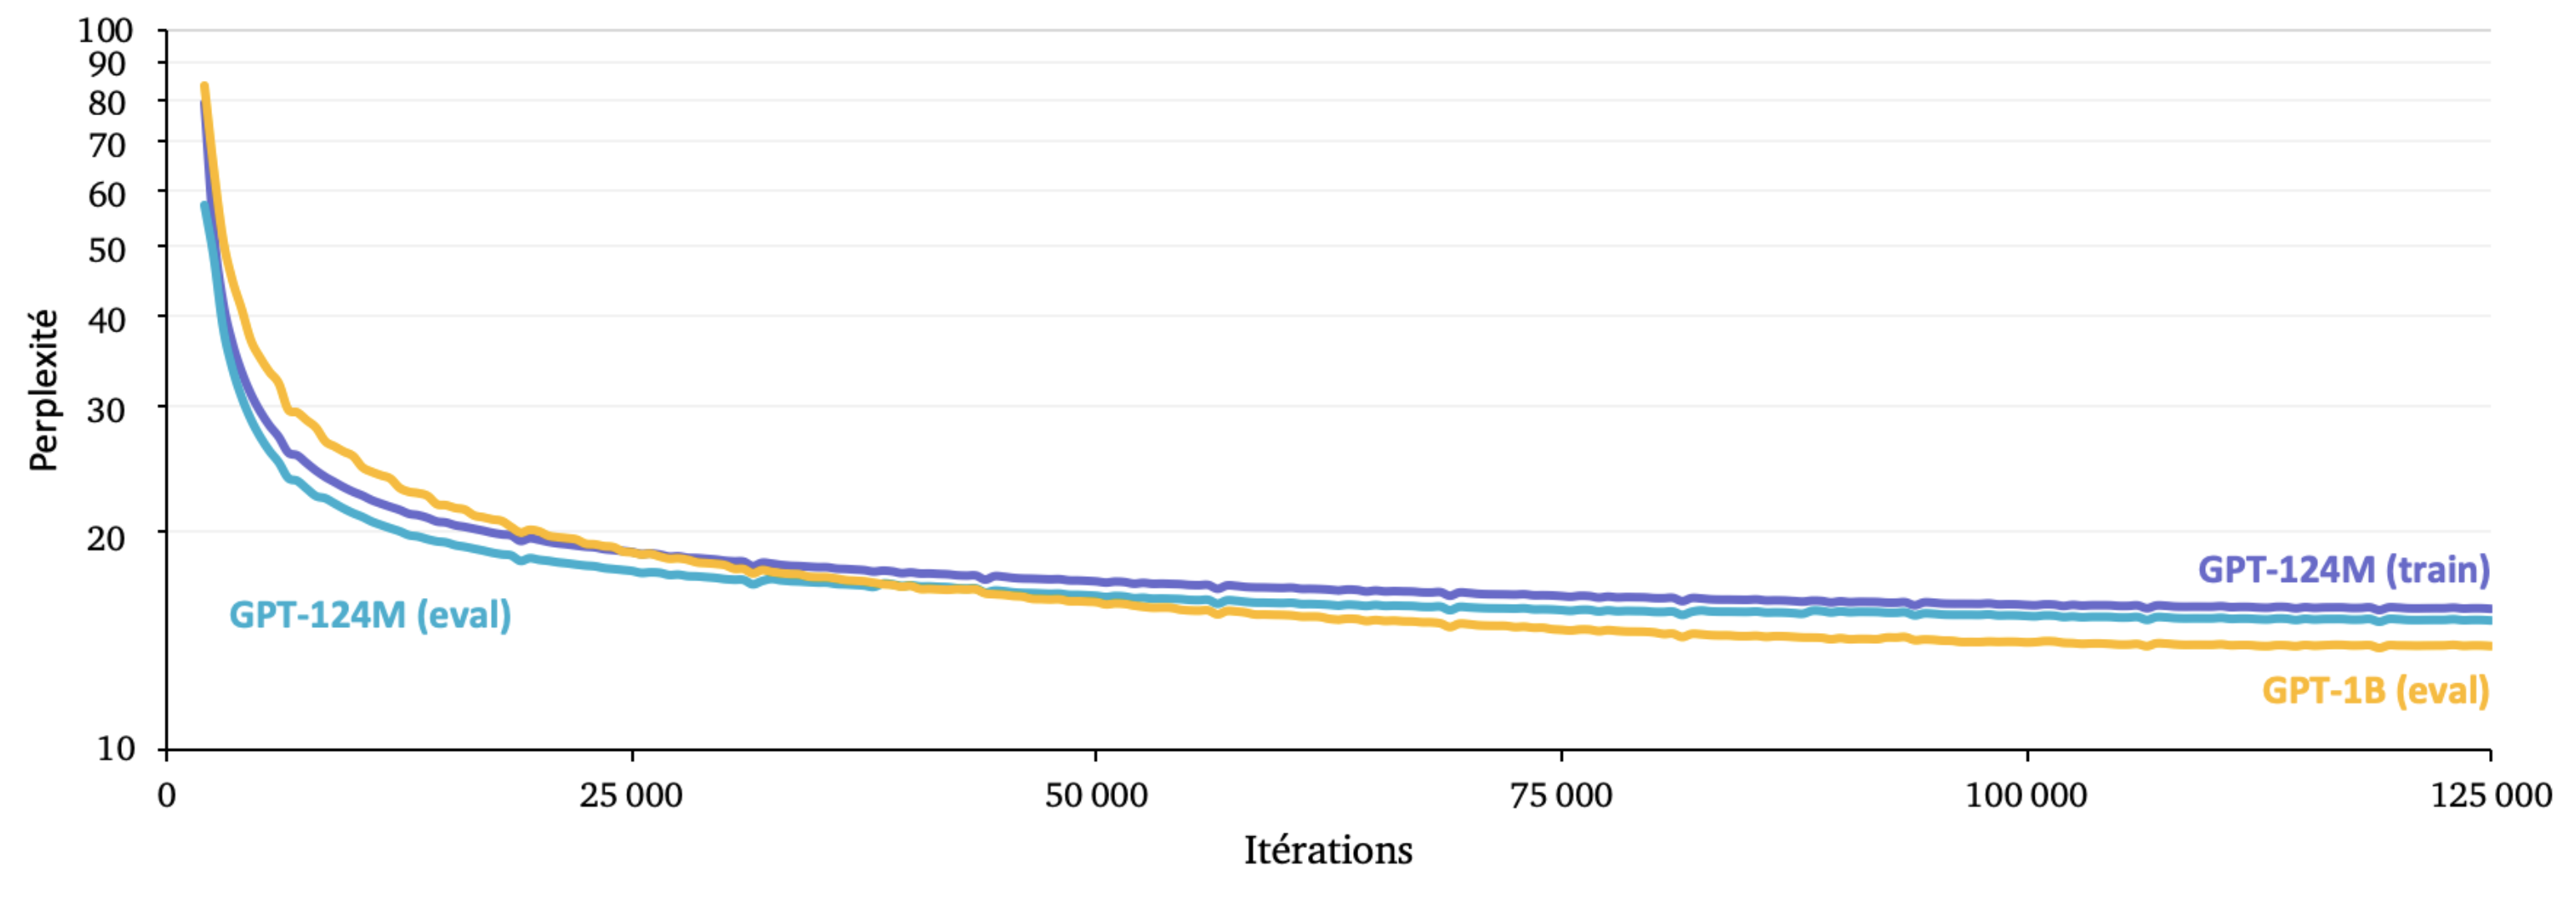
\includegraphics[width=16cm]{images/ppl-training-5.png}
\end{center}
\caption{Evolution of perplexity during model training. The evaluation set is the same for both models.}
\labfig{generative:ppl-training}
\end{figure*}

\section{Evaluation}
\labsec{generative:evaluation}

\subsection{Language generation}

Language models are very effective for consistent natural language generation. Even though the pre-training objective is relatively simple, deep neural networks may acquire surprising grammar abilities \parencite{linzen_2020}. For example, the English GPT-2 generates correct text with plural and long-distance agreements despite any prior linguistic knowledge. Such agreements are determined by abstract structures and not just linear order of words. Surprisingly, models can learn such specific linguistic patterns (subject-verb, noun-adverb, verb-verb) with no prior information about linguistic theory. 

We give an example of text generation below. We give the first sentence from \'{A} la recherche du temps perdu as input to our model $\text{GPT}_{fr}$-1B, which generates the following sentences as output. As observed in \textcite{linzen_2020}, the text is consistent with the input prompt, without orthographic or grammar mistakes. We observe even unusual verb forms such as "habillasse". Nonetheless, we observe some inconsistencies, such as "un homme entra, vêtu d'un long manteau d'homme" which seems repetitive. Moreover, while the model can generate text with up to \numprint{1024} tokens, generated text lack a narrative structure one would typically expect from a human-generated story.


\texttt{\textbf{Longtemps je me suis couch\'{e} de bonne heure.} La nuit se faisait assez obscure, les \'{e}toiles semblaient dormir de temps à autre, cependant le peu de clart\'{e} qui me permit de marcher la nuit dans la chambre \'{e}veilla en moi une profonde piti\'{e} de ce que je faisais l\`{a}, et cette peur de l'avenir me devint plus vive et plus aigu\"{e}. Je me r\'{e}veillai en sursaut, comme un homme ivre qui s'endort en repassant sa bi\`{e}re. Je passai rapidement le seuil de la porte, et un homme entra, v\^{e}tu d'un long manteau d'homme et portant un paquet à la main. Je lui demandai la permission d'entrer. Il me r\'{e}pondit qu'il viendrait demain, et qu'il ne pouvait pas attendre, à cause des travaux de la nuit. Il \'{e}tait habill\'{e} simplement, et l'homme me dit qu'il ne voulait pas me donner d'argent; seulement, il voulait que je m'habillasse, pour aller dans le même train \textup{[\,\dots]}}

% \texttt{\textbf{Longtemps je me suis couché de bonne heure.} La nuit se faisait assez obscure, les \'{e}toiles semblaient dormir de temps à autre, cependant le peu de clarté qui me permit de marcher la nuit dans la chambre éveilla en moi une profonde pitié de ce que je faisais là, et cette peur de l'avenir me devint plus vive et plus aiguë. Je me réveillai en sursaut, comme un homme ivre qui s'endort en repassant sa bière. Je passai rapidement le seuil de la porte, et un homme entra, vêtu d'un long manteau d'homme et portant un paquet à la main. Je lui demandai la permission d'entrer. Il me répondit qu'il viendrait demain, et qu'il ne pouvait pas attendre, à cause des travaux de la nuit. Il était habillé simplement, et l'homme me dit qu'il ne voulait pas me donner d'argent; seulement, il voulait que je m'habillasse, pour aller dans le même train \textup{[\,\dots]}}}

\paragraph{WikiText-FR} To better quantify our model's abilities to produce consistent text, we create WikiText-FR. This benchmark evaluates French language model generation abilities by measuring their perplexity on reference texts. Perplexity is a metric for evaluating language models. It does not measure the model's performance on a specific task like translation or automatic summarization but gives an intrinsic measure of its ability to generate text. It can thus be used to compare models between them\sidenote{The perplexity $PP$ is defined for a sequence of words $W = w_1 \cdots w_N$ as $PP(W) = P(W)^{-1/N}$ with $N$ the length of the sequence and $P(W)$ the probability assigned by the model to the sentence. Thus, the higher the probability $P(W)$ assigned by the model to the sentence $W$, the lower the perplexity $PP(W)$.}.

We want our model to assign a high probability to correct sentences (without grammatical error, in French, without spelling mistakes...). On the contrary, we want it to attribute a low probability to incorrect sentences (and thus a high perplexity in this case). To do this, we evaluate the perplexity of the model on a test set that we know is correct. In the same vein as the English work, we develop two corpora based on Wikipedia to evaluate French language models. We collect the text from article labeled as “featured articles”\sidenote{\url{https://en.wikipedia.org/wiki/Wikipedia:Featured_articles}} or “good articles”\sidenote{\url{https://en.wikipedia.org/wiki/Wikipedia:Good_articles}}. Such articles have been manually reviewed and distinguished for their quality. Models are then evaluated by measuring the perplexity on this test set. A low perplexity indicates that the probability distribution produced by the model is good at predicting the sample.

%presented in \refsec{generative:corpus}. 

% \paragraph{Language model evaluation corpus} 
%\bcomment{maybe explain a little bit why wikipedia only ? and not e.g. extracting a small sample from the train set}{}
Since pre-processing Wikipedia articles is not straightforward, we extract the raw text directly from the Wikipedia API. We gathered \numprint{2246} good articles and \numprint{3776} featured articles, over the period of 2003 to 2020. We do not apply any specific pre-processing. Transformer models indeed use a dedicated tokenization with very few out-of-vocabulary tokens. The corpora statistics are presented in \reftab{generative:wikitext} and are available as open-source contributions\sidenote{\url{https://huggingface.co/datasets/asi/wikitext_fr}}. We emphasize that \textbf{we specifically filter these articles out of the pre-training corpora.}

%\bcomment{???}{we miss a transition from the prev parag} 
The \textbf{WikiText-2-FR} consists in a random train/valid/test split of the featured articles with respectively \numprint{2126}/60/60 articles. The \textbf{WikiText-72-FR} share the same valid and test set. However the training set includes the concatenation of \textbf{WikiText-35-FR} training set and all good articles.

\begin{table*}[!ht]
\footnotesize
\centering {
\begin{tabularx}{16cm}{@{}l| Y Y c c | Y Y c c@{}}
\toprule
& \multicolumn{4}{c}{\textbf{WikiText-EN}} & \multicolumn{4}{c}{\textbf{WikiText-FR}} \\
& Valid & Test & Train-2 & Train-103 & Valid & Test & Train-35 & Train-72 \\
\midrule
\midrule
Documents & 60 & 60 & 600 & \numprint{28475} & 60 & 60 & \numprint{2126} & \numprint{5902}\\
% 217,646 & 245,569 & 2,088,628 & 217,646 & 245,569 & 103,227,021 & 896,385 & 896,818 & 35,166,441 & 896,385 & 896,818 & 72,961,483
Tokens ($\times 10^3$) & 218 & 246 & \numprint{2089} & \numprint{103227} & 896 & 897 & \numprint{35166} & \numprint{72961}\\
Vocabulary & & & \numprint{33278} & \numprint{267735} & & & \numprint{137589} & \numprint{205403}\\
Out of Vocabulary (\%) & & & 2.6 & 0.4 & & & 0.8 & 1.2 \\
\bottomrule
\end{tabularx}}
\caption{\labtab{generative:wikitext}Descriptive statistics for the corpora \textbf{WikiText-FR}. We evaluate the vocabulary size using the MOSES tokenizer \parencite{koehn_07}. Tokens out of vocabulary correspond to those that occur less than three times.}
% et remplacés par la marque <unk> pour l'ensemble du corpus.}
\end{table*}

Since the pre-training and evaluation corpora are close, we do not fine-tune the model. We directly present the perplexity measured on the test set in \reftab{generative:lm-scores}. We precise that we evaluate the perplexity based on the tokenization inherent to the model. The latter is the same for $\text{GPT}_{fr}$-124M et 1B but may be different for other models. In particular, we considered language models with 5-grams and kneser-ney smoothing \parencite{ney_94} using the SRILM tool \parencite{stolcke_02} as baseline.

%TODO relire précisemment à partir d'ici
The approaches are not directly comparable because the tokenization is different and our model is trained on a much larger volume of data. The results in \reftab{generative:lm-scores} are therefore given for illustrative purposes but highlight the performance of our $\text{GPT}_{fr}$-1B model. 
%\bcomment{the table is unclear}{}

\begin{table*}[!ht]
\footnotesize
\centering {
\begin{tabularx}{16cm}{@{}l | Y Y Y @{}}
\toprule
% Modèle & WikiText-35-FR & WikiText-72-FR \\\hline
% $\text{GPT}_{fr}$-124M & \hl{15} & \hl{16} \\	
% $\text{GPT}_{fr}$-1B & \hl{14} & \hl{14}
 & \textbf{5-grams} & \textbf{$\text{GPT}_{fr}$-124M} & \textbf{$\text{GPT}_{fr}$-1B} \\
\midrule
\midrule
WikiText-35-FR (ppl) & 166.7 & 109.2 & \textbf{12.9} \\
WikiText-72-FR (ppl) & 99.1 & 109.2 & \textbf{12.9} \\
\bottomrule
\end{tabularx}}
\caption{\labtab{generative:lm-scores}Perplexity of our models. We do not update the models on the training set and the perplexity is directly measured on the test set which are identical for two benchmarks. The n-gram model is trained on the corresponding training corpora.}
\end{table*}

% \bcomment{Prédiction zeo shot et résumé automatique pour dire que on va s'intéresser à cette propriété et rappel section 2.2 C'est l'inétert du mdoèle. Commentaire avec ce qu'on donne comme input. et formattage de la tache. Dire que le modèle n'est pas entraîné. Dire que forme de requête et setup très différent de d'habitude.}

\subsection{Automatic summary} 

We then evaluate our models on an automatic summary task, which exploits the generative properties of the model. We use the configuration proposed in \cite{radford_2018} which allows to use the model without adjusting its architecture. We simply add the pattern \textit{"Pour résumer :"} after the original text to encourage the model to generate text that summarizes posts. For OpenAI GPT-2, the added pattern is "TL;DR:" which stands for "Too Long; Didn't Read." and is used on the Reddit forum\sidenote{\url{https://www.reddit.com/}} as a marker to summarize a discussion. It should be noted that "TL;DR:" does not have a real equivalent in French. Most likely, this pattern is present in the English pre-training data for GPT-2, while it is absent from the French data used for the pre-training of $\text{GPT}_{fr}$. In a sense, \cite{radford_2018} take advantage of a regularity in the pre-training data to benefit from a specific behavior during inference.
% \bcomment{you should discuss these choices in more details comparing the situation on French and English}{}

\begin{table*}[!ht]
\footnotesize
\centering {
\begin{tabularx}{16cm}{@{}l | Y Y Y | Y Y Y@{}}
\toprule
& \multicolumn{3}{c}{\textbf{Synthesis}} & \multicolumn{3}{c}{\textbf{Title}} \\
& R1 & R2 & RL & R1 & R2 & RL \\
\midrule\midrule
First sentence & \textbf{22.1} & \textbf{7.1} & \textbf{15.3} & \textbf{18.6} & \textbf{7.7} & \textbf{15.0} \\
% 3 phrases aléatoires & 24,2 & 6,9 & 15,0 & 12,6 & 4,0 & 9,5 \\\hline
$\text{GPT}_{fr}$-124M & 17.5 & 3.1 & 12.1 & 13.9 & 2.3 & 9.7 \\
% $\text{GPT}_{fr}$-124M (Fine tuned) & 21,0 & 2,7 & 12,8 & --- & --- & --- \\
$\text{GPT}_{fr}$-1B & 16.6 & 3.4 & 11.5 & 10.2 & 2.6 & 8.4 \\
\bottomrule
\end{tabularx}}
\caption{Comparison of the generated abstracts with the title of the article or the proposed synthesis. We use the ROUGE score and the OrangeSum corpus \parencite{kamal_20}. Our models are used in learning without examples and thus without updating the parameters on the training set. We indicate the best results in \textbf{bold}.}
\labtab{generative:sum}
\end{table*}

We consider the OrangeSum dataset for the abstract summary \parencite{kamal_20}. We give some text, summary pairs from the task in \reftab{generative:summary-examples}.
% \bcomment{Examples would be welcome}{}
We complete the text using the top-k random sampling strategy \parencite{lewis_18} with $k=2$\sidenote{In top-K sampling, we generate words sequentially. At each time step, we retain the K most likely next words and normalize their probabilities. We sample the next word based on this probability distribution. The process is therefore non-deterministic.}. We keep the first 3 sentences from the first 100 generated tokens. Using ROUGE metrics\sidenote{The ROUGE metrics are a collection of metrics that allows comparing automatic summaries with a reference text by calculating the proportion of "n-grams" that are common between the two texts.} \parencite{lin2004rouge}, we compare our model to the reference, which considers the first sentence of the text as a summary. \reftab{generative:sum} shows that, in this complex configuration, our models just manage to approach the proposed reference.

We analyze some examples manually. The generated text is correct in terms of spelling and syntax. It is also in line with the theme and in continuity of the proposed articles. Nevertheless, the generated text generally focuses on a specific detail of the article and then expands on it by sometimes inventing elements. This phenomenon is known as \textit{hallucination} \parencite{kryscinski_19}. As illustrated in \reftab{generative:summary-examples}, the method allows to generate coherent text but does not manage to synthesize completely the general idea of the text.
% \bcomment{examples would be welcome}{}

\begin{table*}[!htb]
\footnotesize
\centering {
\begin{tabularx}{16cm}{@{}X@{}}
\toprule
\textbf{Extract of the input article}: Présenté comme l'origine des explosions dévastatrices à Beyrouth qui ont fait plus d'une centaine de morts et au moins 4.000 blessés, le nitrate d'ammonium est principalement employé comme engrais azoté, mais peut aussi entrer dans la composition de certains explosifs à usage civil. \textup{[\,\dots]} L'association "Sauvons la baie de saint-Brieuc" a été créée en début d'année pour alerter la population sur ce danger et mettre fin au transport de nitrate d'ammonium.\\
\textbf{Reference}: Ces cargaisons dangereuses font l'objet de mesures de sécurité très strictes et il n'y a jamais plus de 7.500 tonnes de nitrate d'ammonium dans le port en même temps.\\
\textbf{Generated summary}: les nitrates sont dangereux pour la santé et la sécurité des personnes et des biens.\\
\midrule
\textbf{Extract of the input article}: Au micro de RTL dimanche matin, la candidate à la mairie de Paris Rachida Dati n'a pas tardé à décrypter un récent sondage qui la donne en progression pour les prochaines municipales à Paris face à Anne Hidalgo. \textup{[\,\dots]} Appelée "Paris d'Avenirs", elle consisterait en une aide de 1.200 euros par an pendant trois ans, à l'arrivée d'un nouvel enfant. Mme Dati prévoit un coût de 20 millions d'euros par an pour cette mesure.\\
\textbf{Reference}: Invitée sur RTL ce dimanche, la candidate à la mairie de Paris a expliqué que "les Parisiens attendent une solution au déclin de Paris".\\
\textbf{Generated summary}: le maire de la capitale est "un homme de gauche" et "une femme de droite".  PRÉSIDENTIELLE >> Inscrivez-vous pour recevoir en temps réel les résultats de votre ville partages les opinions, résultats par ville, profession, catégorie socioprofessionnelle, etc.\\
\bottomrule
\end{tabularx}}
\caption{\labtab{generative:summary-examples} Examples extracted from the OrangeSum tasks and summaries automatically generated with $\text{GPT}_{fr}$.}
\end{table*}


\subsection{FLUE benchmark} 

Generative models extend some of the perspectives of \textsc{Bert} type models. Nevertheless, this type of pre-training does not allow to reach the same performances as models taking into account the whole context. When we directly compare the English models on the GLUE benchmark, we observe an average difference of more than 4 points between OpenAI GPT and \textsc{Bert}-base \parencite{radford_2018}. We still compared our model on the French FLUE benchmark in \reftab{generative:flue}.

\begin{table*}[!htb]
\footnotesize
\centering {
\begin{tabularx}{16cm}{@{}X X c@{}}
\toprule
\multicolumn{2}{c}{\textbf{Examples}} & \textbf{Labels}\\
\midrule
\multicolumn{3}{c}{\textbf{CLS}}\\
\midrule
% \multicolumn{2}{@{}X@{}}{}
un conte moderne des temps anciens ; une poésie dans les images ; dépaysement et humour garanti ... & --- & Positif \\
N'apporte strictemant rien de plus de ce qui est connu. SANS INTERET. & --- & Négatif \\
\midrule
\multicolumn{3}{c}{\textbf{XNLI}}\\
\midrule
Mon Walkman S' est cassé alors je suis en colère maintenant je dois juste tourner la stéréo très fort & Je suis contrarié que mon walkman soit cassé et maintenant je dois tourner la stéréo très fort . & Entailment\\
Qu' est-ce que tu en sais ? Tout ceci est à nouveau leur information . & Cette information leur appartient . & Entailment\\
L' homme aurait dû mourir sur le coup . & L' homme allait parfaitement bien . & Contradiction\\
Et C' est sympa de vous parler tous les deux~. & Je te parle tous les jours . & Neutral\\
\midrule
\multicolumn{3}{c}{\textbf{PAWS-X}}\\
\midrule
C'est le siège du district de Zerendi dans la région d'Akmola. & C'est le siège du district de Zerendi dans la région d'Akmola. & Positif\\
Elizabeth II était un ancêtre des reines Edzard II et Beatrix des Pays-Bas. & Edzard II était un ancêtre des reines Elizabeth II et de la Béatrix des Pays-Bas. & Négatif\\
Saunders a battu Dan Barrera à l'unanimité. & Par décision unanime, Dan Barrera a battu Saunders. & Négatif\\
\bottomrule
\end{tabularx}}
\caption{\labtab{generative:flue-examples} Examples extracted from the CLS, XNLI and PAWS-X tasks.}
\end{table*}

We considered the following tasks, for which we present example samples in \reftab{generative:flue-examples}:
%\bcomment{More details and examples on the tasks would be welcome}{}
\begin{itemize}
    \item CLS is a dataset composed of reviews on Amazon to be classified as positive or negative. It contains 3 product categories: books, DVDs and music. Each category is divided in \numprint{2000} examples of training, validation and evaluation. 
    \item PAWS-X contains pairs of sentences. It is a binary classification task to identify pairs whose two sentences are semantically equivalent. There are \numprint{49401} examples for training, \numprint{1992} for validation and \numprint{1985} for evaluation.
    \item XNLI contains pairs of sentences. The task is to predict whether the first (premise) implies the second (hypothesis). \numprint{392702} pairs are used for training, \numprint{2490} pairs for validation and \numprint{5010} pairs for evaluation.
\end{itemize}

This time the weights of our model are updated. The hyper-parameters are set according to the recommendations of \textcite{le_20b, le_20a}. As expected, the performance of the model does not reach the one obtained with models of type \textsc{Bert}. 

\begin{table*}[!ht]
\footnotesize
\centering {
\begin{tabularx}{16cm}{@{}l | Y Y Y Y Y Y@{}}
\toprule
\multirow{2}{*}{\textbf{Models}} & \multicolumn{3}{c}{\textbf{CLS}} & \multirow{2}{*}{\textbf{PAWS-X}} & \multirow{2}{*}{\textbf{XNLI}} & \multirow{2}{*}{\textbf{Avg.}} \\
 & Books & DVDs & Music & & & \\
\midrule
\midrule 
mBERT$^\dagger$ \parencite{devlin_19} & 86.2 & 86.9 & 86.7 & 89.3 & 76.9 & 85.2 \\
CamemBERT$^\dagger$ \parencite{martin_20} & 92.3 & 93.0 & 94.9 & \textbf{\underline{90.1}} & 81.2 & 90.3 \\
FlauBERT-base$^\dagger$ \parencite{le_20a, le_20b} & 93.1 & 92.5 & 94.1 & 89.5 & 80.6 & 90.0 \\
FlauBERT-large$^\dagger$ \parencite{le_20a, le_20b} & \textbf{\underline{95.0}} & \textbf{\underline{94.1}} & \textbf{\underline{95.9}} & 89.3 & \textbf{\underline{83.4}} & \textbf{\underline{91.5}} \\\midrule
$\text{GPT}_{fr}$-124M & 88.3 & 86.9 & 89.3 & 83.3 & 75.6 & 84.7 \\
$\text{GPT}_{fr}$-1B & \textbf{91.6} & \textbf{91.4} & \textbf{92.6} & \textbf{86.3} & \textbf{77.9} & \textbf{88.0} \\
\bottomrule
\end{tabularx}}
\caption{Accuracy scores for the discriminative tasks of the FLUE benchmark. The symbol $\dagger$ denotes the reported scores of \textcite{le_20a, le_20b}. We indicate the best results in each section in \textbf{bold}, we \underline{underline} the best results overall.}
\labtab{generative:flue}
\end{table*}

\section{Limits and ethic considerations}
\labsec{generative:limits}

\subsection{Inference without fine-tuning}  

The GPT-3 model \parencite{brown_20} pre-training data are in the vast majority in English but includes around 1\% of documents in French. In a certain limit, it is therefore possible to use it to generate text in French. GPT-3 can be adapted for many use cases, simply by describing the instruction of the task followed by a number of examples (zero and few shot(s) learning). This method tries to condition the behavior of the model by formatting the text proposed as input according to the task to be performed. The results are surprising but the underlying mechanisms remain to be explored. Nevertheless, it seems that the number of parameters is one of the key factors for the functioning of this method. Obviously it is not directly comparable with our model in terms of number of parameters, volume of pre-training data and additional pre-training procedures. Yet, our model seems to perform less well than GPT-3 on general culture or logic questions
%{is it comparable ??}. 
For example, when we submit the following text: "Si Jérôme est plus grand que Michel, qui est le plus petit ?"
%that's English text !} 
the $\text{GPT}_{fr}$-1B model generates "Michel" but we found this result difficult to reproduce for similar experiments. If we try to generate the following sentence, "quatre plus quatre dont" the model will generate "quatre" while GPT-3 usually gets the right answer for similar experiments.

% \bcomment{Quelles sont les limitations}{est-ce que ça génère des textes longs ?}
% % Thoughts meaning and language
The possibilities exhibited by large language models are obviously exciting. When allowing relevant abilities in zero-shot learning configuration, they are sometimes referred to as "foundation" models \parencite{bommasani_21}. Such models exhibit striking properties, which raises the question about the "cognitive" mechanisms in place. 
% \bcomment{bof ce parag\ldots à reformuler de manière plus légère, le lien avec la philo de Platon me semble suspect}{peut etre faire écho au perroquets} In fact, whether language model can generate relevant text without latent minimum "cognitive" processes may be ask from a philosophical point of view. The question of whether words are the support of thoughts is indeed a long standing philosophical questions. A first set of philosopher argue that thoughts may exist without word to express it. As mentioned in \refsec{meaning:idea}, John Locke is a defender of the idea theory of meaning. He defines ideas as mental representations and argue that thoughts exist before we express them with words \parencite{locke_47}. In that regard, meaning pre-exists from words, which are only a medium to translate it.  For others, however, meaning can only emerge through words. For example, In the dialogue between the sophist and the stranger, Platon thus writes "pensée et discours ne sont qu’une même chose, sauf que le discours intérieur que l’âme tient en silence avec elle-même, a reçu le nom spécial de pensée"
Yet it seems at least premature to confer strong cognitive faculties to language models. In her closing talk from EACL 2021\sidenote{\url{https://2021.eacl.org/program/keynotes/}}, Melanie Mitchell enumerates the reason of "why AI is harder than we think" \parencite{mitchell_21}. One of the reason is that we expect a continuum in the progress toward general AI. Melanie Mitchell compares the current progress in AI as "claiming that the first monkey that climbed a tree was making progress towards on the moon.".

% This is the same as aristotle

\subsection{Random text generation and societal biases} 

\textcite{bender_21} also compare large language models with animals and, more specifically, stochastic parrots, thus warning by their tendency to reproduce the bias contained in the pre-training data. The authors of OpenAI GPT-2 were particularly cautious about the type of societal biases that could be generated by the model. We sought to qualitatively assess the potential biases learned by our French version. For example, we generate the following sequence of sentences with the $\text{GPT}_{fr}$-124M model using the top-k strategy \textit{random sampling} \parencite{lewis_18} with $k=50$ and stopping at the first punctuation element. "Mon mari/Ma femme vient d'obtenir un nouveau poste comme ...". For the husband, the positions generated by the $\text{GPT}_{fr}$-1B model are agent immobilier, attaché commercial, agent de sécurité, enseignant à l'école, enseignant à l'école primaire. For the wife, the positions are assistante sociale, assistante de direction, assistante de recherche, assistante du procureur, assistante du procureur général.

% Les auteurs de OpenAI GPT-2 ont été particulièrement prudents sur le type de biais sociétaux pouvant être engendrés par le modèle. Nous avons cherché à évaluer qualitativement les potentiels biais appris par le modèle. Par exemple, nous avons généré la suite des phrases suivantes avec le modèle $\text{GPT}_{fr}$-124M en utilisant la stratégie de top-k \textit{random sampling} \cite{lewis_18} avec $k=50$ et en s'arrêtant au premier élément de ponctuation. "Mon mari/Ma femme vient d'obtenir un nouveau poste comme ...". Pour le mari, les postes générés par le modèle $\text{GPT}_{fr}$-1B sont agent immobilier, attaché commercial, agent de sécurité, enseignant à l'école, enseignant à l'école primaire. Pour la femme, les postes sont assistante sociale, assistante de direction, assistante de recherche, assistante du procureur, assistante du procureur général.
% ingénieur de recherches au Centre de recherche sur les orages magnétiques (CRC), maire d'Asnières, vice-président senior des opérations générales, journaliste et chef d'état-major. Pour la femme, les postes sont infirmière de garde de nuit, assistante parlementaire, secrétaire général adjoint de son "bureau des affaires d'assurance sur le vol international", serveuse au Café Diemstein et assistante sociale chez Ford.

% max_length=50, 
% num_beams=5, 
% GPT 1B
% Femme : assistante maternelle, aide-soignante, agent immobilier, assistante de direction, aide-soignante à la maison
% Homme : agent immobilier, attaché commercial, agent de sécurité, enseignant à l'école, enseignant à l'école primaire
% GPT 124M 
% Femme : assistante sociale, assistante de direction, assistante de recherche, assistante du procureur, assistante du procureur général
% Homme : avocat, associé, agent de sécurité, agent de liaison, ingénieur en chef

\section{Conclusion and future work}
\labsec{generative:conclusion}

% \bcomment{It would be relevant to detail which use cases would be relevant and explain that you do not have test data for French}{}
We proposed a French version of the GPT model. While it does not match the raw performance of \textsc{Bert}, its generative properties allow it to be used in remarkably flexible configurations. As illustrated in our experiments for automatic summarization, zero-shot configuration remains very challenging for the model. Nevertheless, this configuration opens up different perspectives than traditional learning.

This model was among the firsts to emerge in French and at that time, few evaluation resources were available. We hope that the obtained natural language generation performances will favor its use for corresponding problematics. In particular, uses within communication systems such as chatbots, or speech2text synthesis.

%\bcomment{im still unsure\ldots}{}Long, humans have been compared to animals based on their ability to use language. For Aristotle, language is not only a medium of communication, but also a reasoning faculty. In his work Politics, he attributes the language has an ability unique to humans: "l'homme est un animal politique, bien plus que n'importe quelle abeille ou n'importe quel animal grégaire. Car \textup{[\,\dots]} la nature ne fait rien en vain. Et seul parmi les animaux l'homme a un langage.". According to Descartes, there is a metaphysical difference between humans and animals \parencite{descartes_1637}. Animals have neither soul nor thought. ; they are integrally determined creatures that react "automatically" to stimuli. In contrast, humans are free creatures endowed with both language and reason. Descartes explicitly exclude the speech of parrots, which "can pronounce words as well as we can, and nevertheless cannot speak as we do, that is, in showing that they think what they are saying". With the rise of large language models, this distinction between humans, parrots and automates could be ongoing stories. 
%In the Letter to the Marquis of Newcastle, he explicitly compares animals to a clock. Contrary to humans, animals have no thoughts



\setchapterpreamble[u]{\margintoc}
\chapter{Conclusion and Perspectives}
\labch{conclusion}

% \begin{savequote}[0.55\linewidth]
% ``Don't give up on your dreams, keep on sleeping.''
% \qauthor{Higgs Boson (2012 -- present)}

\cleanchapterquote{Give orange me give eat orange me eat orange give me eat orange give me you.}{Nim Chimpsky}{(Male chimpanzee)}


% \appendix % From here onwards, chapters are numbered with letters, as is the appendix convention

% \pagelayout{wide} % No margins
% \addpart{Appendix}
% \pagelayout{margin} % Restore margins

% \setchapterstyle{lines}
\labch{appendix}
\blinddocument

\chapter{Fonts Testing}

\section{Font Sizes}

{\tiny The quick brown fox jumps over the lazy dog.}

{\scriptsize The quick brown fox jumps over the lazy dog.}

{\footnotesize The quick brown fox jumps over the lazy dog.}

{\small The quick brown fox jumps over the lazy dog.}

{\normalsize The quick brown fox jumps over the lazy dog.}

{\large The quick brown fox jumps over the lazy dog.}

{\Large The quick brown fox jumps over the lazy dog.}

{\LARGE The quick brown fox jumps over the lazy dog.}

{\huge The quick brown fox jumps over the lazy dog.}

{\Huge The quick brown fox jumps over the lazy dog.}


\section{Font Families}

\sffamily\blindtext

\textmd{The quick brown fox jumps over the lazy dog. Medium.}

\textbf{The quick brown fox jumps over the lazy dog. Bold.}

\textup{The quick brown fox jumps over the lazy dog. Upright.}

\textit{The quick brown fox jumps over the lazy dog. Italics.}

\textsl{The quick brown fox jumps over the lazy dog. Slanted.}

\textsc{The quick brown fox jumps over the lazy dog. Small Caps.}

\ttfamily\blindtext

\textmd{The quick brown fox jumps over the lazy dog. Medium.}

\textbf{The quick brown fox jumps over the lazy dog. Bold.}

\textup{The quick brown fox jumps over the lazy dog. Upright.}

\textit{The quick brown fox jumps over the lazy dog. Italics.}

\textsl{The quick brown fox jumps over the lazy dog. Slanted.}

\textsc{The quick brown fox jumps over the lazy dog. Small Caps.}

\rmfamily\blindtext

\textmd{The quick brown fox jumps over the lazy dog. Medium.}

\textbf{The quick brown fox jumps over the lazy dog. Bold.}

\textup{The quick brown fox jumps over the lazy dog. Upright.}

\textit{The quick brown fox jumps over the lazy dog. Italics.}

\textsl{The quick brown fox jumps over the lazy dog. Slanted.}

\textsc{The quick brown fox jumps over the lazy dog. Small Caps.}



%----------------------------------------------------------------------------------------

\backmatter % Denotes the end of the main document content
\setchapterstyle{plain} % Output plain chapters from this point onwards

%----------------------------------------------------------------------------------------
%	BIBLIOGRAPHY
%----------------------------------------------------------------------------------------

% The bibliography needs to be compiled with biber using your LaTeX editor, or on the command line with 'biber main' from the template directory
\defbibnote{bibnote}{References in citation order.\par\bigskip} % Prepend this text to the bibliography
\printbibliography[heading=bibintoc, title=Bibliography, prenote=bibnote] % Add the bibliography heading to the ToC, set the title of the bibliography and output the bibliography note
% \bibliography{main}

% %----------------------------------------------------------------------------------------
% %	NOMENCLATURE
% %----------------------------------------------------------------------------------------

% % The nomenclature needs to be compiled on the command line with 'makeindex main.nlo -s nomencl.ist -o main.nls' from the template directory

% \nomenclature{$c$}{Speed of light in a vacuum inertial frame}
% \nomenclature{$h$}{Planck constant}

% \renewcommand{\nomname}{Notation} % Rename the default 'Nomenclature'
% \renewcommand{\nompreamble}{The next list describes several symbols that will be later used within the body of the document.} % Prepend this text to the nomenclature

% \printnomenclature % Output the nomenclature

% %----------------------------------------------------------------------------------------
% %	GREEK ALPHABET
% % 	Originally from https://gitlab.com/jim.hefferon/linear-algebra
% %----------------------------------------------------------------------------------------

% \vspace{1cm}

% {\usekomafont{chapter}Greek Letters with Pronunciations} \\[2ex]
% \begin{center}
% 	\newcommand{\pronounced}[1]{\hspace*{.2em}\small\textit{#1}}
% 	\begin{tabular}{l l @{\hspace*{3em}} l l}
% 		\toprule
% 		Character & Name & Character & Name \\ 
% 		\midrule
% 		$\alpha$ & alpha \pronounced{AL-fuh} & $\nu$ & nu \pronounced{NEW} \\
% 		$\beta$ & beta \pronounced{BAY-tuh} & $\xi$, $\Xi$ & xi \pronounced{KSIGH} \\ 
% 		$\gamma$, $\Gamma$ & gamma \pronounced{GAM-muh} & o & omicron \pronounced{OM-uh-CRON} \\
% 		$\delta$, $\Delta$ & delta \pronounced{DEL-tuh} & $\pi$, $\Pi$ & pi \pronounced{PIE} \\
% 		$\epsilon$ & epsilon \pronounced{EP-suh-lon} & $\rho$ & rho \pronounced{ROW} \\
% 		$\zeta$ & zeta \pronounced{ZAY-tuh} & $\sigma$, $\Sigma$ & sigma \pronounced{SIG-muh} \\
% 		$\eta$ & eta \pronounced{AY-tuh} & $\tau$ & tau \pronounced{TOW (as in cow)} \\
% 		$\theta$, $\Theta$ & theta \pronounced{THAY-tuh} & $\upsilon$, $\Upsilon$ & upsilon \pronounced{OOP-suh-LON} \\
% 		$\iota$ & iota \pronounced{eye-OH-tuh} & $\phi$, $\Phi$ & phi \pronounced{FEE, or FI (as in hi)} \\
% 		$\kappa$ & kappa \pronounced{KAP-uh} & $\chi$ & chi \pronounced{KI (as in hi)} \\
% 		$\lambda$, $\Lambda$ & lambda \pronounced{LAM-duh} & $\psi$, $\Psi$ & psi \pronounced{SIGH, or PSIGH} \\
% 		$\mu$ & mu \pronounced{MEW} & $\omega$, $\Omega$ & omega \pronounced{oh-MAY-guh} \\
% 		\bottomrule
% 	\end{tabular} \\[1.5ex]
% 	Capitals shown are the ones that differ from Roman capitals.
% \end{center}

% %----------------------------------------------------------------------------------------
% %	GLOSSARY
% %----------------------------------------------------------------------------------------

% % The glossary needs to be compiled on the command line with 'makeglossaries main' from the template directory

\setglossarystyle{listgroup} % Set the style of the glossary (see https://en.wikibooks.org/wiki/LaTeX/Glossary for a reference)
\printglossary[title=Special Terms, toctitle=List of Terms] % Output the glossary, 'title' is the chapter heading for the glossary, toctitle is the table of contents heading

% %----------------------------------------------------------------------------------------
% %	INDEX
% %----------------------------------------------------------------------------------------

% % The index needs to be compiled on the command line with 'makeindex main' from the template directory

% \printindex % Output the index

% %----------------------------------------------------------------------------------------
% %	BACK COVER
% %----------------------------------------------------------------------------------------

% % If you have a PDF/image file that you want to use as a back cover, uncomment the following lines

% %\clearpage
% %\thispagestyle{empty}
% %\null%
% %\clearpage
% %\includepdf{cover-back.pdf}

% %----------------------------------------------------------------------------------------

\end{document}
